% !TEX program = pdflatex
%!TEX root = main.tex

\documentclass[9pt]{extarticle}

\usepackage{natbib}
\bibliographystyle{abbrvnat}
\setcitestyle{authoryear} %Citation-related commands open={((},close={))}

\usepackage[nottoc]{tocbibind}

\usepackage[a4paper, left=25mm, right=25mm,  top=25mm, bottom=25mm, headsep=5mm] {geometry} 

\usepackage{fancyhdr}
\usepackage{lastpage}
\usepackage{svg}
\usepackage[font=footnotesize]{caption}
\usepackage{graphicx}
\usepackage{pdfpages}
\usepackage{subcaption}
\usepackage{color,soul}
\usepackage{wrapfig}
\usepackage{subcaption}
\usepackage{amsmath}
\usepackage{physics}
\usepackage{mathrsfs}
\usepackage{tabularx}
\usepackage{multirow}
\usepackage{multicol}
\usepackage{xurl}
\usepackage{hyperref}
\usepackage{amssymb}
\hypersetup{
    colorlinks=true,
    linkcolor=black,
    citecolor=black,      
    urlcolor=cyan
    }
\usepackage{graphicx}

\usepackage{xcolor}
\usepackage{pdfpages}
\usepackage{enumitem}

\usepackage{listings}
\usepackage{matlab-prettifier}

\usepackage{float}

\usepackage{silence}
\WarningFilter{caption}{Unused}

\usepackage{tikz}
\usetikzlibrary{patterns,decorations.pathmorphing,positioning}

\newcommand{\mycomment}[1]{}

\usepackage{arydshln}

%% ----------  Packages above --------

% Define a general page style with both header and footer
\fancypagestyle{otherpages}{
\fancyhf{} % clear all header and footer fields
\renewcommand{\headrulewidth}{0pt} % remove header rule
\fancyfoot[C]{} % Clear the center footer field
\fancyfoot[R]{Page \thepage \space of \pageref*{LastPage}}}
\pagestyle{otherpages}% Apply the general page style to all pages by default


\begin{document}

\begin{titlepage} % CAPA

\centering


\begin{figure}
 \centering
 
\includegraphics[width=0.30\textwidth]{Figures/Logo_IST_color.jpg}
\end{figure}


{ \rule{\linewidth}{0.5mm} }

{\Huge\bfseries Development of Control Strategies for Seismic Reproduction on Seismic Platform \par}
\vspace{0.2cm}
{\huge\bfseries \par}
\vspace{0.5cm}
{\scshape\huge Design of Mechatronic Systems\par} %

\vspace{1cm}

\begin{figure}[H]
 \centering
 \fbox{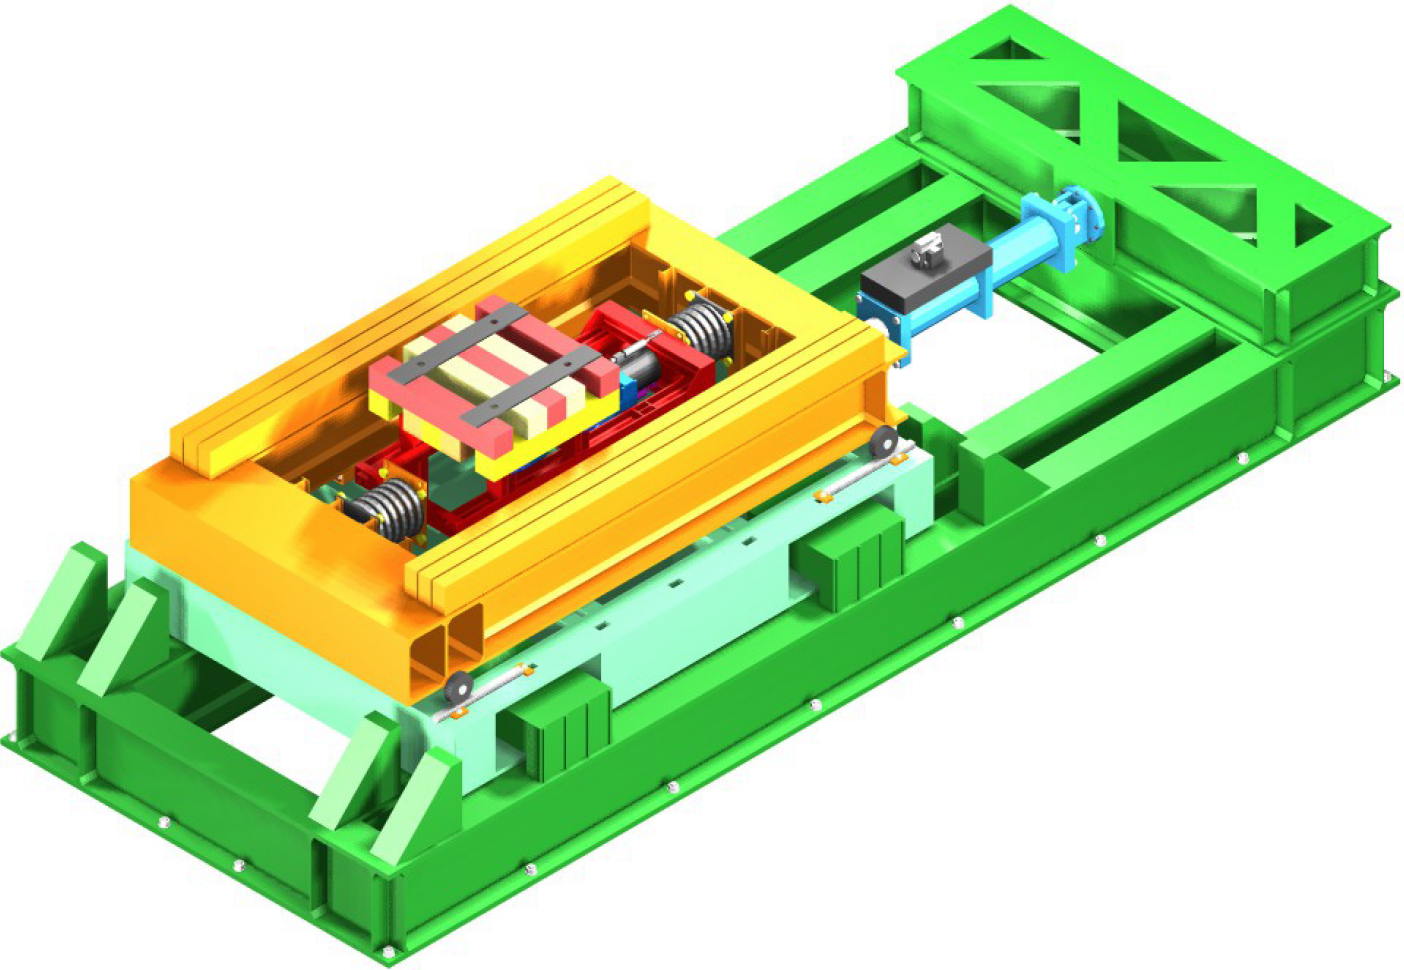
\includegraphics[width=0.8\textwidth]{Figures/capa.png}}  %imagem de capa
\end{figure}

\vspace{1cm} 

% Autores
\vspace{.2cm}

\huge Afonso Costa Henrique \\
\href{mailto:afonso.henrique@tecnico.ulisboa.pt}{\Large afonso.henrique@tecnico.ulisboa.pt}\par
%\href{https://github.com/c-radicallis/Controlo_Plataforma_Sismica}{\large  Repository} {\large  \&}  \href{https://www.overleaf.com/read/scyrtvmjtzgc#eef70f}{\large  Report}\par
\vspace{10mm}


Supervisors: \\
\vspace{2mm}
\Large
{Miguel Ayala Botto  - \href{mailto:ayalabotto@tecnico.ulisboa.pt}{ayalabotto@tecnico.ulisboa.pt}}\\
\vspace{1mm}
{Fernando Pires de Oliveira  - \href{mailto:fvoliveira@lnec.pt}{fvoliveira@lnec.pt}}     \\


\vspace{.7cm}

\vfill {\large October 2024\par} %Data

\end{titlepage}
\setcounter{page}{2}
\clearpage
%%%%%%%%%%%%%%%%%%%%%%%%%%%%%%%%%%%%%%%%%%%%%%%%%%%%%%%%%%%%%%%%%%%%%%%%%%%%%%%%%%%%%%%%%
 
%  %AGRADECIMENTOS
 
% \vfill % pushes following text to bottom

% \begin{center}
    
% Aos meus supervisores, Miguel e Fernando, que me trouxeram a este projeto e sempre me guiaram

% Ao Paulo Candeias, um poço de conhecimento e uma ajuda indispensável

% Aos meus pais, que me deram a possibilidade de estudar

% \vspace{5mm}

% Eternamente grato
% \end{center}
% \clearpage

%%%%%%%%%%%%%%%%%%%%%%%%%%%%%%%%%%%%%%%%%%%%%%%%%%%%%%%%%%%%%%%%%%%%%%%%%%%%%%%%%%%%%%%%%

\section{Resumo}

texto aqui

\textbf{Palavras Chave:} words, words

%%%%%%%
\clearpage
\section{Abstract}

text here

\textbf{Keywords:} words, words

%%%%%%%%%%%%%%%%%%%%%%%%%%%%%%%%%%%%%%%%%%%%%%%%%%%%%%%%%%%%%%%%%%%%%%%%%%%%%%%%%%%%%%%%%
\clearpage
\tableofcontents % Indice
%\clearpage

\listoftables % Tabelas
%\clearpage
    
\listoffigures %Figuras
%\clearpage

%%%%%%%%%%%%%%%%%%%%%%%%%%%%%%%%%%%%%%%%%%%%%%%%%%%%%%%%%%%%%%%%%%%%%%%%%%%%%%%%%%%%%%%%%


\clearpage
\section{Introduction}

\subsection{The Experimental Setup at LNEC}
The current seismic platform testing process at Laboratório Nacional de Engenharia Civil (LNEC) consists of synthesizing a drive signal, distinct from the reference signal, so that the platform replicates the response spectra of the reference signal, i.e. the earthquake. %The system comprising the seismic platform and the structure to be tested uses a proportional controller with fixed parameters.

\begin{figure}[H]
    \centering
    \fbox{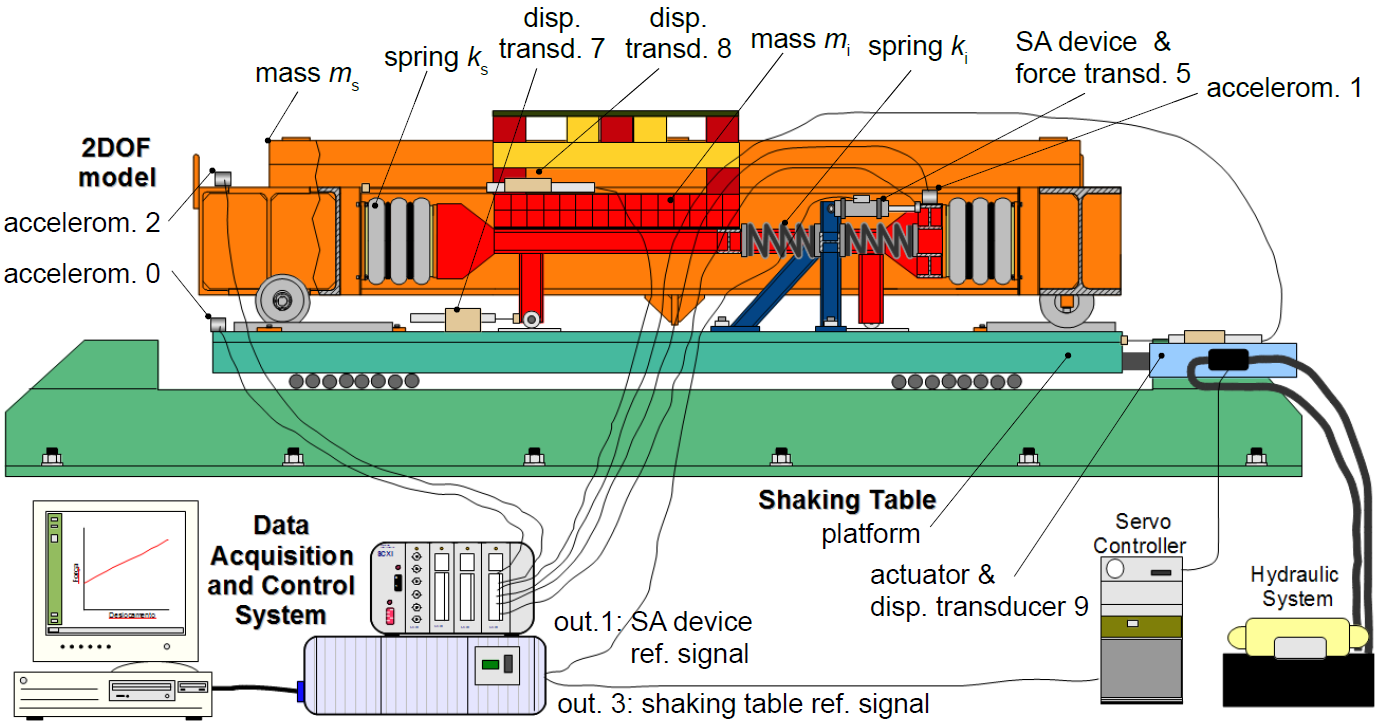
\includegraphics[width=0.9\linewidth]{Intro/schematic_st1d_Fernando.png}}
    \caption{Complete schematic representation of uniaxial shaking table (1D-ST) with a coupled 2DOF system \citep{oliveira2015}}
    \label{fig_schematic_st1d_Fernando}
\end{figure}

During the seismic test, the structure is subjected to a series of tests with different earthquake amplitudes. Initially, the test is carried out with the earthquake at a reduced amplitude, assessing the subsequent damage. The procedure is then repeated with the same earthquake, but at a higher amplitude, again assessing the damage, and so on until a defined amplitude is reached, which usually corresponds to the original amplitude of the earthquake.

Before each test, an identification of the system's transfer function is carried out, using a limited-band white noise signal.%, always with the same amplitude, to determine the system's transfer function.
This function is then used in the command signal generation algorithm. Throughout this process, the amplitude of the reference signal increases progressively, and it is expected that the structure will enter a non-linear regime, either due to the behaviour of some of its components or the damage accumulated during the various tests.

\begin{figure}[H]
\begin{minipage}{0.4\textwidth}
    \centering
    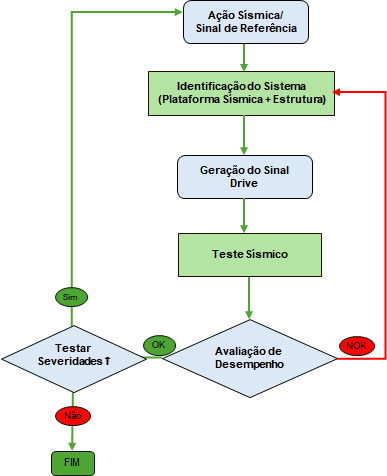
\includegraphics[width=\linewidth]{Intro/schematic_test_process.png}
    \caption{Work flow diagram of the seismic testing process at LNEC}
    \label{schematic_test_process}
\end{minipage}
\hfill
\begin{minipage}{0.55\textwidth} \setlength{\parindent}{4pt}

\hspace*{\parindent} At the end of each test, the system's performance is evaluated by comparing the response spectrum of the reference signal with that of the signal measured on the platform. However, it is not always possible to achieve satisfactory performance with the command signal synthesized initially, and it may be necessary to generate more than one command signal and carry out additional tests at the same amplitude. This procedure, although necessary in some situations, should be avoided as it induces additional damage to the structure.

\hspace*{\parindent} In addition, the system faces physical limitations inherent to the equipment, namely with regard to the finite field of displacement, velocity and acceleration, which must be duly considered during the tests.

\hspace*{\parindent} At the end of each test, the system's performance is evaluated by comparing the response spectrum of the reference signal with that of the signal measured on the platform. However, it is not always possible to achieve satisfactory performance with the command signal synthesized initially, and it may be necessary to generate more than one command signal and carry out additional tests at the same amplitude. This procedure, although necessary in some situations, should be avoided as it induces additional damage to the structure.

\end{minipage}
\end{figure}

%\hspace*{\parindent} 
In addition, the system faces physical limitations inherent to the equipment, namely with regard to the finite field of displacement, velocity and acceleration, which must be duly considered during the tests.

%\hspace{\parindent}
Before each test, an identification of the system's transfer function is carried out using band-limited white noise.%, always with the same amplitude, to determine the system's transfer function.
This transfer function is then used in the command signal generation algorithm. Throughout this process, the amplitude of the reference signal increases progressively, and it is expected that the structure will enter a non-linear regime, either due to the behaviour of some of its components and the accumulated damage during the various tests.


%\hspace{\parindent} 
At the end of each test, the system's performance is evaluated by comparing the response spectrum of the reference signal with that of the signal measured on the platform. However, it is not always possible to achieve satisfactory performance with the command signal synthesized initially, and it may be necessary to generate more than one command signal and carry out additional tests at the same amplitude. This procedure, although necessary in some situations, should be avoided as it induces additional damage to the structure.

%\hspace{\parindent} 
In addition, the system faces physical limitations inherent to the equipment, namely with regard to the finite field of displacement, velocity and acceleration, which must be duly considered during the tests.

\begin{figure}[H]
\begin{minipage}{0.6\textwidth}
\setlength{\parindent}{2pt}
%\vspace{-10mm}
\subsection{Response Spectrum}% in Civil Engineering} %\subsection{Key Aspects of Response Spectrum}

\hspace*{\parindent} The \textbf{response spectrum} is a fundamental concept in earthquake engineering and structural dynamics. It represents the maximum response (such as displacement, velocity, or acceleration) of a structure modelled as a single-degree-of-freedom (SDOF) system subjected to a ground motion. 

It's relevance for this work lies in the fact that the performance of the seismic table, will be assessed mostly based on it's ability to reproduce seismic ground motion response spectra, which will be evaluated for frequencies between 0.1 and 30 Hz.

\vspace{5mm}

\hspace*{\parindent} Figure \ref{fig_response_spectrum_schematic} helps us easily comprehend how a response spectrum is determined.  The peak amplitudes {\textcircled{\raisebox{-.9pt}{3}}}, from the response of  1-DoF mass-spring-damper systems with 5\% damping and different natural frequencies {\textcircled{\raisebox{-.9pt}{2}}}, to the seismic signal {\textcircled{\raisebox{-.9pt}{1}}}, are plotted for the each natural frequency {\textcircled{\raisebox{-.9pt}{4}}}.

\vspace{5mm}

\hspace*{\parindent} Some fundamental concepts on response spectrum are:
\begin{itemize}[noitemsep, topsep=0pt, leftmargin=*]
    \item Ground Motion Dependency
    \begin{itemize}[noitemsep, topsep=0pt, leftmargin=*]
        \item It is derived from an earthquake acceleration time history.
        \item Different earthquakes produce different response spectra.
    \end{itemize}
    
    \item Structures Dynamic Properties
    \begin{itemize}[noitemsep, topsep=0pt, leftmargin=*]
        \item The response depends on the structure’s \textbf{natural frequency} and \textbf{damping ratio}.
        \item Structures with different natural periods respond differently to the same ground motion.
    \end{itemize}

    \item Spectral Parameters
    The response spectrum can show maximum values of:
    \begin{itemize}[noitemsep, topsep=0pt, leftmargin=*]
        \item Spectral Acceleration: Used for force-based design.
        \item Spectral Velocity: Important for energy-based considerations.
        \item Spectral Displacement: Relevant for displacement-based design.
    \end{itemize}
\end{itemize}

\vspace{5mm}
%\subsection{Applications in Civil Engineering}
\hspace*{\parindent} Some of its applications in Civil Engineering are:
\begin{itemize}[noitemsep, topsep=0pt, leftmargin=*]
    \item Seismic Design of Buildings and Bridges: Response spectra help in defining design forces.
    \item Code Based Seismic Analysis: Building codes (e.g., \textit{ASCE 7, Eurocode 8, IS 1893}) provide standard response spectra.
    \item Performance Based Seismic Design (PBSD): Uses response spectra to predict structural behavior.
\end{itemize}

\end{minipage}
\hspace{10mm}
\begin{minipage}{0.3\textwidth}
    \centering
    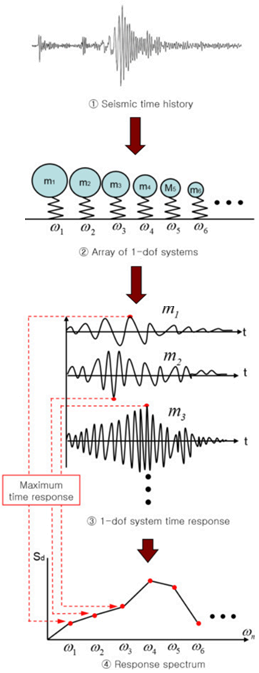
\includegraphics[width=\textwidth]{response_spectrum_schematic.png}
    \caption{ Schematized process of determining a response spectrum }
    \label{fig_response_spectrum_schematic}
\end{minipage}
\end{figure}

\clearpage


\subsection{Objectives}
The objective of this work is to implement a controller, or strategy, to ensure that the seismic platform reproduces the test seismic signal (reference/earthquake) as accurately as possible, taking into account the following aspects:
\begin{itemize}
    \item The amplitude of the earthquake increases progressively with each test during the experimental campaign;
    \item Before each test, an identification of the system is carried out at a reduced amplitude (to avoid damaging the model). One objective will be to assess the feasibility of using the earthquake response to identify, or complement the identified model, and cover higher amplitudes.
    \item The command signal, generated offline, is imposed on the seismic platform without prior evaluation, by simulation, as to its effectiveness in creating the desired output at the seismic platform;
    \item The seismic platform system with 1 degree of freedom (ST1D) is capable of testing models with a mass of up to 5 tons, and operates in a band of interest from 0 to 25 Hertz. It also has the following limitations (which should be confirmed in laboratory tests):
    \begin{itemize}
        \item Maximum displacement, in absolute value, of 100 mm
        \item Maximum speed, in absolute value, of 0.4 m/s
        \item Maximum acceleration, in absolute value, of 25 m/s$^2$
    \end{itemize}
    \item The model to be tested may initially exhibit linear behaviour, but as it degrades, it inevitably becomes non-linear. In general, the structures tested have two vibration modes in the seismic platform's band of interest, whose initial characteristics (without damage) are:
    \begin{itemize}[label=$\diamond$]
    \item $1.5 \leq f_1 (\mathrm{Hz}) \leq 4$
    \item $2 \leq \xi_1 (\%) \leq 5$
    \item $6 \leq f_2 (\mathrm{Hz}) \leq 10$
    \item $5 \leq \xi_2 (\%) \leq 15$
    
    In damaged structures, damping can reach:
    \begin{itemize}
        \item $\xi_1 = 10\%$
        \item $\xi_2 = 25\%$
    \end{itemize}
    \end{itemize}

    \item Performance will be evaluated by comparing the response spectrum of the measured signal with that of the reference signal.
\end{itemize}


%\clearpage
\section{State of the Art} %\section{Revisão do Estado da Arte}\label{sec:sota}
%Realizar uma pesquisa abrangente sobre técnicas para ensaios sísmicos, com foco em ensaios em plataforma sísmica. Incluir uma análise dos métodos de ensaio, configurações de montagem, bem como da instrumentação utilizada para medição e controlo dos equipamentos.

\subsection{Simulation and Reality: The role of experimental testing in seismic engineering}
% IS SEISMIC EXPERIMENTAL TESTING OF STRCUTURES STILL NECESSARY, DESPITE THE EVOLUTION OF COMPUTACIONAL SIMULATIONS?
% https://consensus.app/search/is-seismic-experimental-testing-of-strcutures-stil/L-Ya5EyiQSqxujE68BaTQw/?utm_source=share&utm_medium=clipboard
While computational simulations have become highly sophisticated and efficient, they still face limitations in accurately modelling complex, nonlinear, or poorly understood behaviours, especially in components with significant uncertainties or novel materials. 
Studies show that numerical simulations, even with advanced methods, require experimental benchmarks to ensure accuracy, especially for complex interactions. Machine learning approaches also rely on experimental data for training and updating models. Experimental testing provides critical validation and calibration for these models.

In summary, seismic experimental testing remains indispensable for validating models, understanding complex behaviours, and ensuring structural safety. The trend is toward integrated approaches using both experimental and computational tools to achieve the most reliable seismic performance assessments.\citep{williams2001,Zhang2023Experimentally,Liu2020Experimental,Bahraq2021Numerical,Malomo2022M-DEM,Qiu2024Seismic,Yavas2023A,Mokhtari2023A}


\subsection{An Overview of Experimental Methods}
% IN THE FIELD OF SEISMIC ENGINEERING, WHAT ARE THE MOST WIDELY USED EXPERIMENTAL METHODS?
% https://consensus.app/search/in-the-field-of-seismic-engineering-what-are-the-m/QdpmhhJsS76N_XJJZcAGgA/
According to \cite{williams2001}, the most widely used experimental methods in the field of seismic engineering are:
\begin{itemize}
    \item \textbf{Shaking Table Tests:} Shaking tables simulate real earthquake ground motions on structural or soil models, allowing direct observation of dynamic response and failure mechanisms. They are considered the gold standard for dynamic testing of buildings, bridges, tunnels, and other infrastructure. 
    They are used for both full-scale and scaled models, including innovative in-situ testing with mobile shaking tables \citep{williams2001,Bousias2017Experimental,Abovyan2024Method,Tsinidis2020Seismic,DeFelice2016Methods,El-Emam2018Experimental}. 

    \item \textbf{Pseudo-Dynamic Testing} and \textbf{Hybrid Simulation:} In pseudo-dynamic testing, loads are applied over a greatly expanded time scale with the dynamic behaviour of the structure accounted for computationally. In hybrid simulation, just like pseudo-dynamic testing, a combination of physical testing and numerical modelling is used, but the experimental part of the process is performed at the correct rate so that the test specimen can respond dynamically. These methods are widely used for complex or large structures where full dynamic testing is impractical \citep{williams2001,Bousias2017Experimental}.

    \item \textbf{Static and Cyclic Loading Tests:} These tests apply static or cyclic loads to materials, structural elements, or systems to study their properties under earthquake-like conditions \citep{williams2001,Bousias2017Experimental,Fiorino2016Experimental}.

    \item \textbf{Centrifuge Modelling:} Centrifuge tests use scaled soil-structure models spun at high speeds to replicate gravitational stresses, enabling realistic simulation of soil-structure interaction during earthquakes, especially for underground structures such as tunnels. This method is mostly focused on testing soil properties, not structures \citep{williams2001,Tsinidis2020Seismic}.

    \item \textbf{Surface Based Seismic Methods:} Used for site characterization, through passive-source (microtremor) and active-source techniques, to determine ground shear-wave velocity profiles \citep{Luke2008Characterizing}.
    
    \item \textbf{Laboratory Fault Slip Experiments:} Used to study fault mechanics and induced seismicity, employing shear-flow, triaxial, and injection-driven tests \citep{Ji2022Laboratory,Dong2022Investigations}.
    
    \item \textbf{Vibration Machines:} Employed for simulating seismic impacts on buildings and models, offering a cost-effective alternative for certain applications \citep{Abovyan2024Method}.

    \item \textbf{Explosive Charges:} Arrays of explosive charges used to simulate earthquake ground motions at large scale (very uncommon method) \citep{williams2001}.
\end{itemize}


% SEISMIC TABLE CONTROL FOR DYNAMIC TESTING OF STRUCTURES & CAN ADAPTIVE CONTROL IMPROVE SHAKING TABLE TEST ACCURACY?
% https://consensus.app/search/adaptive-control-shaking-tables/P-JOknr3Slax_foG1eKOKg/?utm_source=share&utm_medium=clipboard

\subsection{Control Strategies and Innovations}
Advanced control methods, such as active disturbance rejection control (ADRC), adaptive model-based state estimators, and nonlinear signal-based control, have significantly improved the accuracy and stability of shaking table operations, especially for reproducing complex seismic waveforms and handling nonlinear structural responses %619
. Offline iterative control and frequency-splitting techniques enable double-layer shaking tables to achieve both high payload and wide frequency range, addressing the needs of testing rigid structures like dams and nuclear facilities %14
. Proportional-derivative (PD) control and affordable hardware have made seismic table testing more accessible in resource-limited settings %18
.


% \subsubsection{Can adaptive control improve shaking table test accuracy?}
% Yes, adaptive control can significantly improve the accuracy of shaking table tests for dynamic structural evaluation.
Adaptive control has been shown to significantly improve the accuracy of shaking table tests for dynamic structural evaluation:
\begin{itemize}
    \item Enhanced Tracking and Stability: Adaptive control methods, such as adaptive-model-based state estimators, model reference adaptive control, and adaptive sliding mode control, have been shown to improve both the stability and tracking accuracy of shaking tables, especially under varying test conditions and nonlinear system behaviors %1456891415+2 MORE.
    \item Compensation for Uncertainties: Adaptive controllers can dynamically adjust to compensate for amplitude and phase deviations, system nonlinearities, and parameter uncertainties, leading to more precise seismic waveform reproduction and better handling of control-structure interaction effects %161418.
    \item     Superior Performance over Conventional Methods: Comparative studies demonstrate that adaptive control strategies outperform traditional fixed-parameter controllers (such as PID or three-variable controllers) in both time and frequency domains, providing better acceleration tracking and robustness to specimen uncertainties %4561314.
    \item     Practical Validation: Experimental and simulation results across multiple studies confirm that adaptive control approaches—such as online adaptive compensation, adaptive inverse control, and functional link adaptive controllers—consistently yield higher fidelity in replicating target motions and structural responses during shaking table tests %15789101113+5 MORE.
\end{itemize}




\section{Modelling Seismic Table Dynamics}\label{Modelling Seismic Table Dynamics}
%\section{Modelação Matemática}
%Os modelos devem ser implementados em Matlab/Simulink e complementados com funções, scripts e interfaces que facilitem a parametrização, cálculo de propriedades (como modos de vibração), análise e simulação com diferentes tipos de entradas (sinais sinusoidais, ondas quadradas e inputs externos como sinais sísmicos).

\subsection{Previous Works}

In \cite{oliveira2015} a complete schematic representation of the ST1D, with a coupled 2DOF system, and instrumentation, can be found (figure \ref{fig_schematic_st1d_Fernando}).

In \citet{tekeste2021} a model for the ST1D with a coupled 1DOF system %rigidly attached payload
is devised from linearized analytical models for each of its components (controller, servo valve, hydraulic actuator, platen mass, and total damping). 

\begin{figure}[H]
    \centering
    \fbox{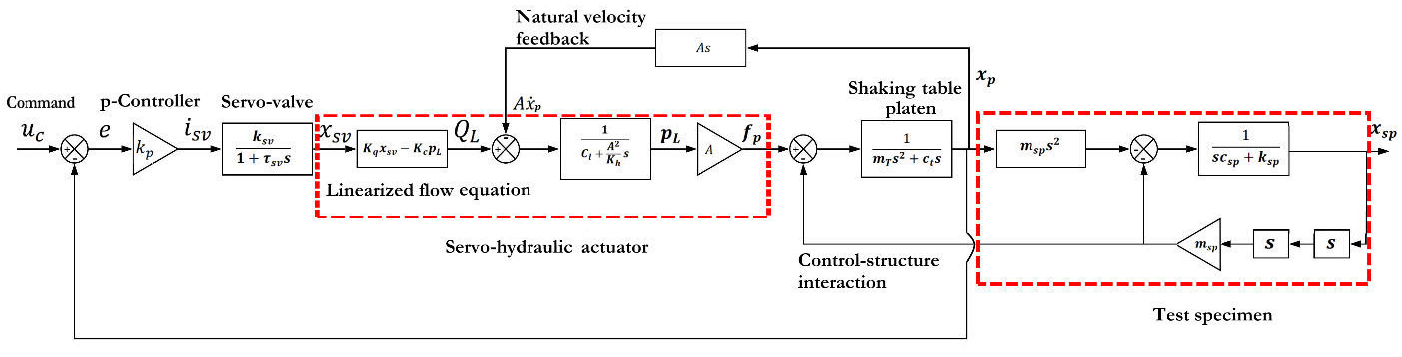
\includegraphics[width=0.98\linewidth]{Modelling/Gidewon_block_diagram.png}}
    \caption{Schematic diagram of a shaking table system with payload rigidly attached \citep{tekeste2021}}
    \label{fig_Tekeste_block_diagram}
\end{figure}

In the previously mentioned publication, the parameters in table \ref{tab:parameters} were determined for the model in figure \ref{fig_Tekeste_block_diagram}. 

It's important to note that the servo valve and hydraulic actuators have since been updated.  Until a new identification of the updated system has been performed, the parameters determined in \cite{tekeste2021} are the ones which will be used in all simulation studies.

\begin{table}[H]
\centering
\caption{ST1D model parameters \citep{tekeste2021}}
\begin{tabular}{|c|l|c|}
\hline
\textbf{Symbol} & \textbf{Description} & \textbf{Value (Units)} \\ \hline
$k_p$ & Proportional gain of the controller & $1.2993 \, \text{V/cm}$ \\ \hline
$k_{sv}$ & Servo-valve gain &  \\ \hline % 1934.50 \,
$\tau_{sv}$ & Time-delay parameter of the servo-valve transfer function & $0.0246 \, \text{s}$ \\ \hline
$k_{sv}k_q$ & Valve flow gain & $1934.50 \, \text{cm}^3/\text{s/V}$ \\ \hline % 
$k_c$ & Valve pressure-flow gain &   \\ \hline %$\text{m}^3/\text{s/kPa}$
$C_l$ & Total leakage coefficient of the piston &  \\ \hline %$ \text{m}^3/\text{s/kPa}$
$ k_{Pl}$ & $ = k_c + C_l $ & $ 1.67401\cdot 10^{-7}   \text{m}^3/\text{s/kPa} $\\ \hline
$A$ & Area of the fluid under compression in the actuator & $0.012456 \, \text{m}^2$ \\ \hline
$V_t$ & Total volume of the fluid under compression in the actuator & $0.002659 \, \text{m}^3$ \\ \hline
$\beta_e$ & Effective bulk modulus of the system & $193716.28 \, \text{kPa}$ \\ \hline
$K_h$ & Oil-column frequency of the actuator & $4531.79 \, \text{kPa/m}$ \\ \hline
$m_p$ & Mass of the platen & $1.9751 \, \text{ton}$ \\ \hline
$c_t$ & Combined damping force of the actuator and the platen & $5.7800 \, \text{kNs/m}$ \\ \hline
$k_{sp}$ & Stiffness of the SDOF structure & - \\ \hline
$c_{sp}$ & Damping of the SDOF structure & - \\ \hline
$m_t^*$ & Total mass considering the payload (shaking table) & - \\ \hline
$H_{sp}$ & Transfer function relating platen and SDOF structure displacement & - \\ \hline
\end{tabular}
\label{tab:parameters}
\end{table}


A \textit{Simulink} model %(Figure \ref{fig_simulink_tekeste}) of the block diagram in Figure \ref{fig_Tekeste_block_diagram} 
was built in order to simulate the ST1D dynamics, however, its implementation resulted in a build up of numerical errors leading to overflow, making this modelling approach unviable.

% \begin{figure}[H]
%     \centering
%     \fbox{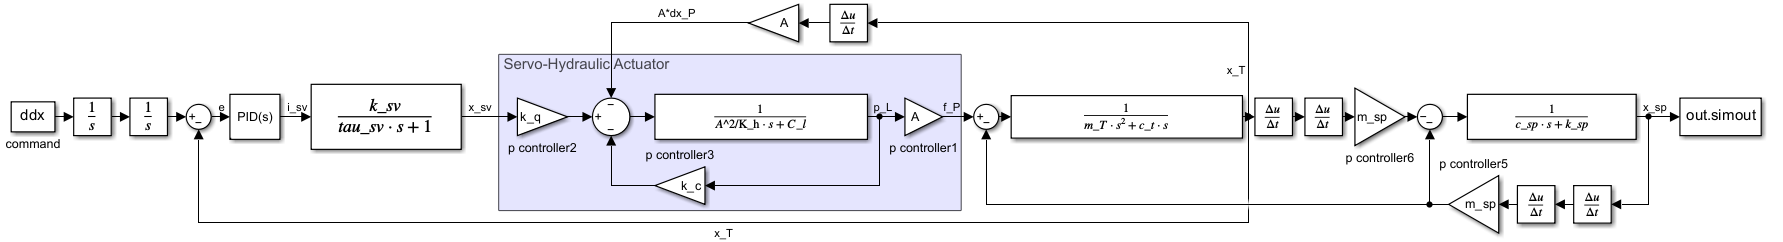
\includegraphics[width=0.98\linewidth]{simulink_1dof_model.png}}
%     \caption{\textit{Simulink} model of the ST1D}
%     \label{fig_simulink_tekeste}
% \end{figure}

\subsection{Mathematical Model for LNEC Uniaxial Seismic Table with a Coupled 2DoF System}

Given the previous results, an alternative approach was found in order to simulate the system, which consisted on obtaining the transfer function relating the desired platen position, $x_{ref}$, as input, and the force applied to the platen, $F_P$, as output.

\begin{figure}[H]
    \centering
    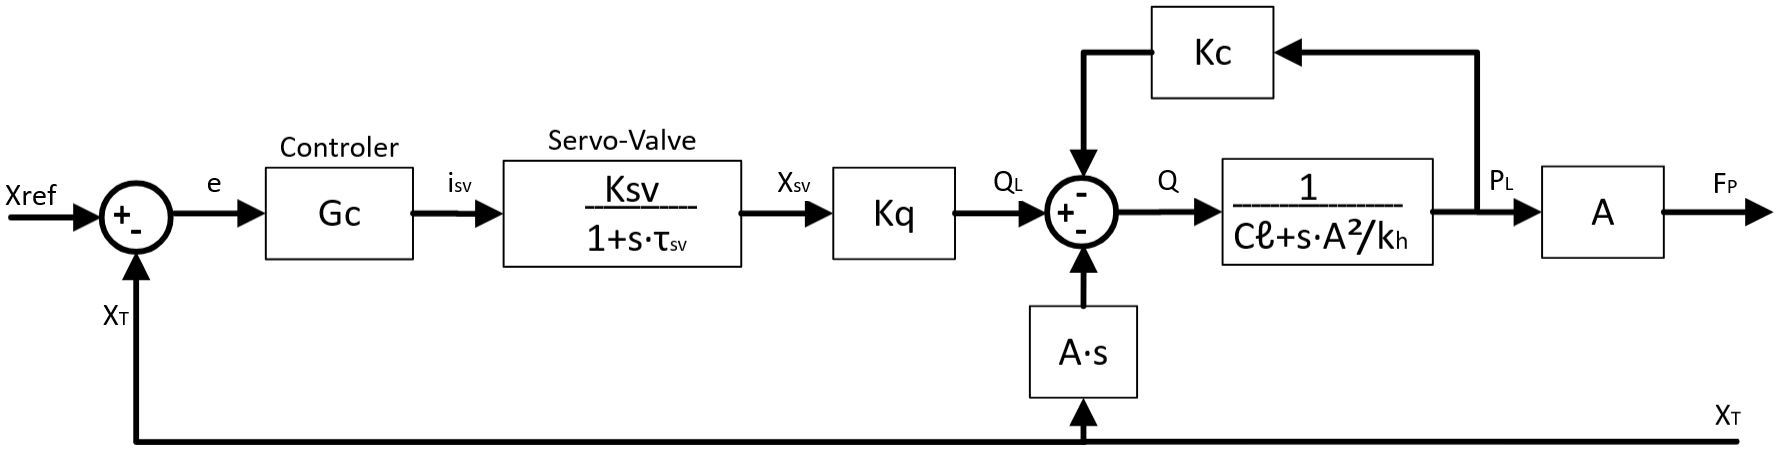
\includegraphics[width=0.7\linewidth]{Modelling/ST1D_block_diagram.png}
    \caption{Block diagram of the ST1D}%, with position $X_{ref}$ as input and force applied to the platen $F_P$ as output.
    \label{fig_clean_block_force_output}
\end{figure}

From the block diagram in figure \ref{fig_clean_block_force_output}, the following equations were derived:


\begin{align}
\left\{
    \begin{aligned}
        G_C(s) &= \frac{i_{sv}}{e} = \frac{i_{sv}}{x_{\text{ref}} - x_T} \\
        \frac{Q_L}{x_{\text{ref}} - x_T} &= \frac{Q_L}{e} = K_q \cdot \frac{K_{\text{sv}}}{1 + \tau_{\text{sv}} s} \cdot G_C(s) \\
    \end{aligned}
\right.
\Longrightarrow G_{csv}(s) &=  \frac{Q_L}{e} = \frac{k_{sv} k_q G_c}{1 + \tau_{sv} s} 
\end{align}

\begin{align}\label{eq_G_Fp_isv}
    \begin{aligned}
    & P_L = \frac{1}{C_l + \frac{A^2}{k_h}\cdot s} [Q_L - A \cdot s \cdot x_T - k_c \cdot P_L] \Longleftrightarrow \\
    & \Longleftrightarrow \frac{F_P}{i_{sv}} = \frac{A \cdot \frac{k_{sv} k_q}{1 + \tau_{sv} s} } {  k_{Pl} + \frac{A^2}{k_h}\cdot s  + A^2\cdot s \cdot G_{xT/Fp}} = G_{Fp/i_{sv}}(s) \quad \text{, where $k_{Pl}=k_c + C_l$}
    \end{aligned}
\end{align}

It's important to note that the transfer function $G_{Fp/i_{sv}}(s)$  is also a function of the model coupled to the platform (see equations \ref{eq_G_Fp_isv} \& \ref{G_xT_Fp}).

To represent the dynamics of a typical structure on test(which has two vibration modes in the bandwidth of the seismic table), a 2 degree of freedom mass-spring-damper system is coupled to the platen, as depicted in figure \ref{schematic_2dof}:

\begin{figure}[H]
\centering
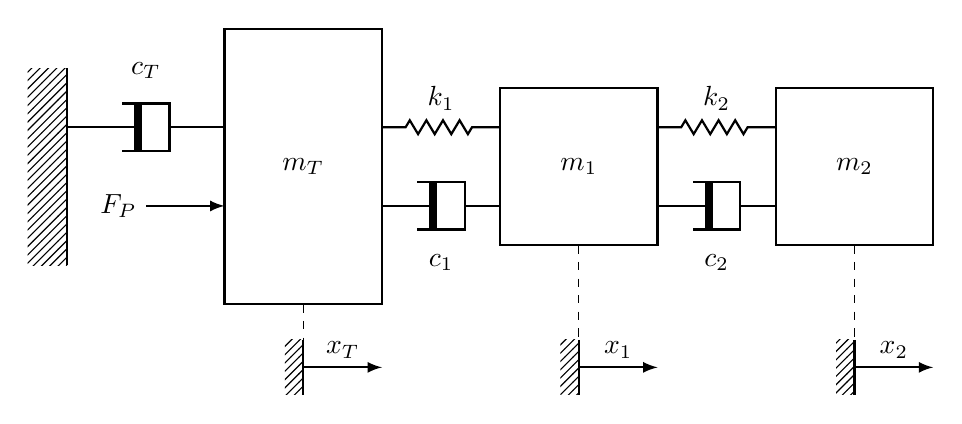
\begin{tikzpicture}[
    every node/.style={outer sep=0pt}, thick, % Set default node style and line thickness
    mass/.style={draw, thick}, % Define style for masses (rectangles)
    spring/.style={thick, decorate, decoration={zigzag, pre length=0.3cm, post length=0.3cm, segment length=6}}, % Define style for springs
    ground/.style={fill, pattern=north east lines, draw=none, minimum width=0.75cm, minimum height=0.3cm}, % Define style for ground
    dampic/.pic={ % Define a small pictogram for a damper
        \fill[white] (-0.1,-0.3) rectangle (0.3,0.3);
        \draw (-0.3,0.3) -| (0.3,-0.3) -- (-0.3,-0.3);
        \draw[line width=1mm] (-0.1,-0.3) -- (-0.1,0.3);
    }
]

    % Define the mass blocks
    \node[mass, minimum width=2cm, minimum height=3.5cm] (mT) {$m_T$}; % First mass 
    \node[mass, minimum width=2cm, minimum height=2cm, right=1.5cm of mT] (m1) {$m_1$}; % Second mass
    \node[mass, minimum width=2cm, minimum height=2cm, right=1.5cm of m1] (m2) {$m_2$}; % Third mass

    % Define the ground (left of mT)
    \node[left=2cm of mT, ground, minimum width=5mm, minimum height=25mm ] (ground) {}; 
    \draw (ground.north east) -- (ground.south east); % Draw vertical edge of the ground block


    % Connect the ground to mT with a damper
    \draw ([yshift=5mm]ground.east) coordinate(aux) -- (mT.west|-aux) 
        pic[midway]{dampic} node[midway, above=5mm]{$c_T$}; % Damper from ground to mT

    % Draw springs between elements
    \draw[spring] (mT.east|-aux) -- (m1.west|-aux) node[midway, above=1mm]{$k_1$}; % Spring from mT to m1
    \draw[spring] (m1.east|-aux) -- (m2.west|-aux) node[midway, above=1mm]{$k_2$}; % Spring from m1 to m2

    % Draw dampers in parallel with the springs
    \draw ([yshift=-5mm]mT.east) coordinate(aux') -- (m1.west|-aux') 
        pic[midway]{dampic} node[midway, below=5mm]{$c_1$}; % Damper from mT to m1
    \draw (m1.east|-aux') -- (m2.west|-aux') 
        pic[midway]{dampic} node[midway, below=5mm]{$c_2$}; % Damper from m1 to m2

    % Define a common baseline for displacement markers
    \coordinate (disp_line) at ([yshift=-8mm]mT.south);
    % Draw displacement markers inline using common baseline
    \foreach \X in {T,1,2} {  
        \draw[thin, dashed] (m\X.south) -- (m\X.south |- disp_line); % Align displacement lines
        \draw[latex-] (m\X.east |- disp_line) -- ++ (-1,0) node[midway, above]{$x_\X$} % Labels for x_T, x_1, x_2
            node[left, ground, minimum height=7mm, minimum width=1mm] (g'\X){};
        \draw[thick] (g'\X.north east) -- (g'\X.south east); 
    }

    % Draw force input on mT
    \draw[latex-] ([yshift=-5mm]mT.west) -- ++ (-1,0) node[left]{$F_P$}; % Force applied to mT
\end{tikzpicture}
\caption{Schematic representation of the 2 degree of freedom mass-spring-damper system coupled to the platen}
\label{schematic_2dof}
\end{figure}


%\vspace{5mm}
For the system in figure \ref{schematic_2dof} the following equations of motion are obtained (system of equations \ref{eq_2dof_system}):

\begin{align}\label{eq_2dof_system}
\left\{
\begin{aligned}
    m_T \cdot \ddot{x}_T &+ c_T \cdot \dot{x}_T + c_1 (\dot{x}_T -  \dot{x}_1) + k_1 (x_T - x_1) = F_p \\
    m_1 \cdot \ddot{x}_1 &+ c_1 ( \dot{x}_1 -\dot{x}_T) + c_2 ( \dot{x}_1 - \dot{x}_2) + k_1 (x_1 - x_T) + k_2 (x_1 - x_2) = 0 \\
    m_2 \cdot \ddot{x}_2 &+ c_2 ( \dot{x}_2 -\dot{x}_1) + k_2 (x_2 - x_1) = 0
\end{aligned}
\right. 
\Longleftrightarrow
\end{align}

\vspace{5mm}

\begin{equation*} 
\Longleftrightarrow
\left\{
\begin{aligned}
    &m_T  \ddot{x}_T + (c_T + c_1)  \dot{x}_T + k_1 x_T - c_1  \dot{x}_1 - k_1  x_1 = F_p \\
    &m_1  \ddot{x}_1 + (c_1 + c_2) \dot{x}_1 + (k_1 + k_2) x_1 - c_1  \dot{x}_T - c_2  \dot{x}_2 - k_1  x_T - k_2 x_2 = 0 \\
    &m_2  \ddot{x}_2 + c_2 \dot{x}_2 + k_2 x_2 - c_2  \dot{x}_1 - k_2 x_1 = 0
\end{aligned}
\right.
\Longleftrightarrow
\end{equation*}

\vspace{5mm}

\begin{equation*}
\Longleftrightarrow
\begin{bmatrix}
    m_T & 0 & 0 \\
    0 & m_1 & 0 \\
    0 & 0 & m_2
\end{bmatrix}
\begin{bmatrix}
    \ddot{x}_T \\ \ddot{x}_1 \\ \ddot{x}_2
\end{bmatrix}
+
\begin{bmatrix}
    c_T + c_1 & -c_1 & 0 \\
    -c_1 & c_1 + c_2 & -c_2 \\
    0 & -c_2 & c_2
\end{bmatrix}
\begin{bmatrix}
    \dot{x}_T \\ \dot{x}_1 \\ \dot{x}_2
\end{bmatrix}
+
\begin{bmatrix}
    k_1 & -k_1 & 0 \\
    -k_1 & k_1 + k_2 & -k_2 \\
    0 & -k_2 & k_2
\end{bmatrix}
\begin{bmatrix}
    x_T \\ x_1 \\ x_2
\end{bmatrix}
=
\begin{bmatrix}
    F_p \\ 0 \\ 0
\end{bmatrix}
\end{equation*}

    
\vspace{5mm}
From the system of equations \ref{eq_2dof_system}, the following transfer functions relating the displacements of the each mass to the displacements of an adjacent mass, or the force applied to the platen, are obtained:

\begin{minipage}{0.49\textwidth}

\begin{align}
    \frac{x_T}{F_P} &= \frac{G_1 G_2 - G_{21}^2}{G_T G_1 G_2 - G_T G_{21}^2 - G_2 G_{T1}^2} = G_{xT/Fp}(s) \label{G_xT_Fp}\\
    \frac{x_1}{x_T} &= \frac{G_{T1} G_2}{G_1 G_2 - G_{21}^2} = G_{x1/xT}(s) \\
    \frac{x_2}{x_1} &= \frac{G_{21}}{G_2} = G_{x2/x1}(s)
\end{align}
\end{minipage}
\hfill
\begin{minipage}{0.49\textwidth}
\begin{align}
    G_T(s) &= m_T\cdot s^2 + (c_T + c_1)\cdot s + k_1 \\
    G_1(s) &= m_1\cdot s^2 + (c_1 + c_2)\cdot s + k_1 + k_2 \\
    G_2(s) &= m_2\cdot s^2 + c_2\cdot s + k_2 \\
    G_{T1}(s) &= c_1\cdot s + k_1 \\
    G_{21}(s) &= c_2\cdot s + k_2 
\end{align}
\end{minipage}


\begin{align}
    G_{Fp/x_{ref}}(s) &= \frac{G_{csv}}{\frac{k_{pl}}{A} + \frac{A}{k_h} s + G_{xT/Fp} (G_{csv} + A\cdot s)} \\
    G_{xT/x_{ref}}(s) &= G_{Fp/x_{ref}} \cdot G_{xT/Fp} 
    %\\
    % G_{x1/x_{ref}}(s) &= G_{x1/xT} \cdot G_{xT/x_{ref}} \\
    % G_{x2/xT}(s) &= G_{x2/x1} \cdot G_{x1/xT}
\end{align}

The mass $m_i$, stiffness $k_i$, and damping $c_i$, of each element will be determined such that the system's natural frequencies $f_i$ and damping ratios $\xi_i$ are similar to the structures in test. Equation \ref{eq_modal_frequencies} relates the natural frequency of the two modes of the 2DoF system to it's spring and mass properties, and equation \ref{eq_modal_damping} relates the damping coefficient and ratio to mass and natural frequency.

\begin{equation}\label{eq_modal_frequencies}
\omega_{1,2}^{2} = \frac{1}{2}\frac{m_1 k_2 + m_2 (k_1 + k_2)}{m_1 m_2} \mp \frac{1}{2} \sqrt{\left( \frac{m_1 k_2 + m_2 (k_1 + k_2)}{m_1 m_2} \right)^2 - 4 \frac{k_1 k_2}{m_1 m_2}} 
\end{equation}

\begin{equation}\label{eq_modal_damping} 
    \xi_i = \frac{ c_i}{2\cdot m_i\cdot \omega_i}
\end{equation}

\section{Evaluating Controller Performance in Simulation Environment}\label{Evaluating Controller Performance in Simulation Environment}

\subsection{Tuned PIDF}

For a preliminary analysis of the mathematical model, some simulations were run using the seismic data from the 1979  Imperial Valley Earthquake, El Centro (Described in \cite{narasimhan2006} \& available \href{https://github.com/c-radicallis/Controlo_Plataforma_Sismica}{here}), which was scaled down to $73.51\%$, in order to comply with the displacement range of the seismic table. Table \ref{tab:modal_params} contains the parameters for the 2DOF coupled structure (Figure \ref{schematic_2dof}).

\begin{table}[H]
    \centering
    \renewcommand{\arraystretch}{1.3}
    \begin{tabular}{|c|c|c|}
        \hline
        \textbf{System Properties} & \textbf{1st Mode} & \textbf{2nd Mode} \\
        \hline
        Frequency ($f_i$) [Hz] & $4$ & $10$ \\
        \hline
        Damping Ratio ($\zeta_i$) & $0.02$ & $0.05$ \\
        \hline
        \textbf{Element's Properties} & \textbf{Element 1} & \textbf{Element 2} \\
        \hline
        Mass ($m_i$) [kg] & $2000$ & $2000$ \\
        \hline
        Stiffness ($k_i$) [N/m] & $3.30\cdot 10^5$ & $1.89\cdot 10^6$ \\
        \hline
        Damping Coefficient ($c_i$) [N$\cdot$m/s] & $1.26\cdot 10^3$ & $1.26\cdot 10^4$ \\
        \hline
    \end{tabular}
    \caption{Modal parameters for the system, and resulting stiffness and damping for each element}
    \label{tab:modal_params}
\end{table}

Initially the simulations were run with the controller set as $G_c(s)=129.93$ V/m, which is the tune typically used at LNEC. Afterwards, a simulation was run with $G_c(s)$ as:
\begin{equation}
    G_c(s) = K_p +  \frac{K_i}{s} +  \frac{K_d\cdot s}{T_f\cdot s + 1} \quad \text{ where: $Kp = 1540, Ki = 1670, Kd = 17.9 , Tf = 6.96\cdot10^{-5}$}
\end{equation}
Where the parameters $K_p, K_i, K_d$ and $T_f$ were obtained using MATLAB's \textit{pidtune} function, with the tuning option \textit{'DesignFocus'} set to \textit{'reference-tracking'}. This results are labelled as "tuned" in figures \ref{fig_response_spectrum_of_3} through to \ref{fig_Platen_Displacement_Tracking_Error}.

\begin{figure}[H]
    \centering
    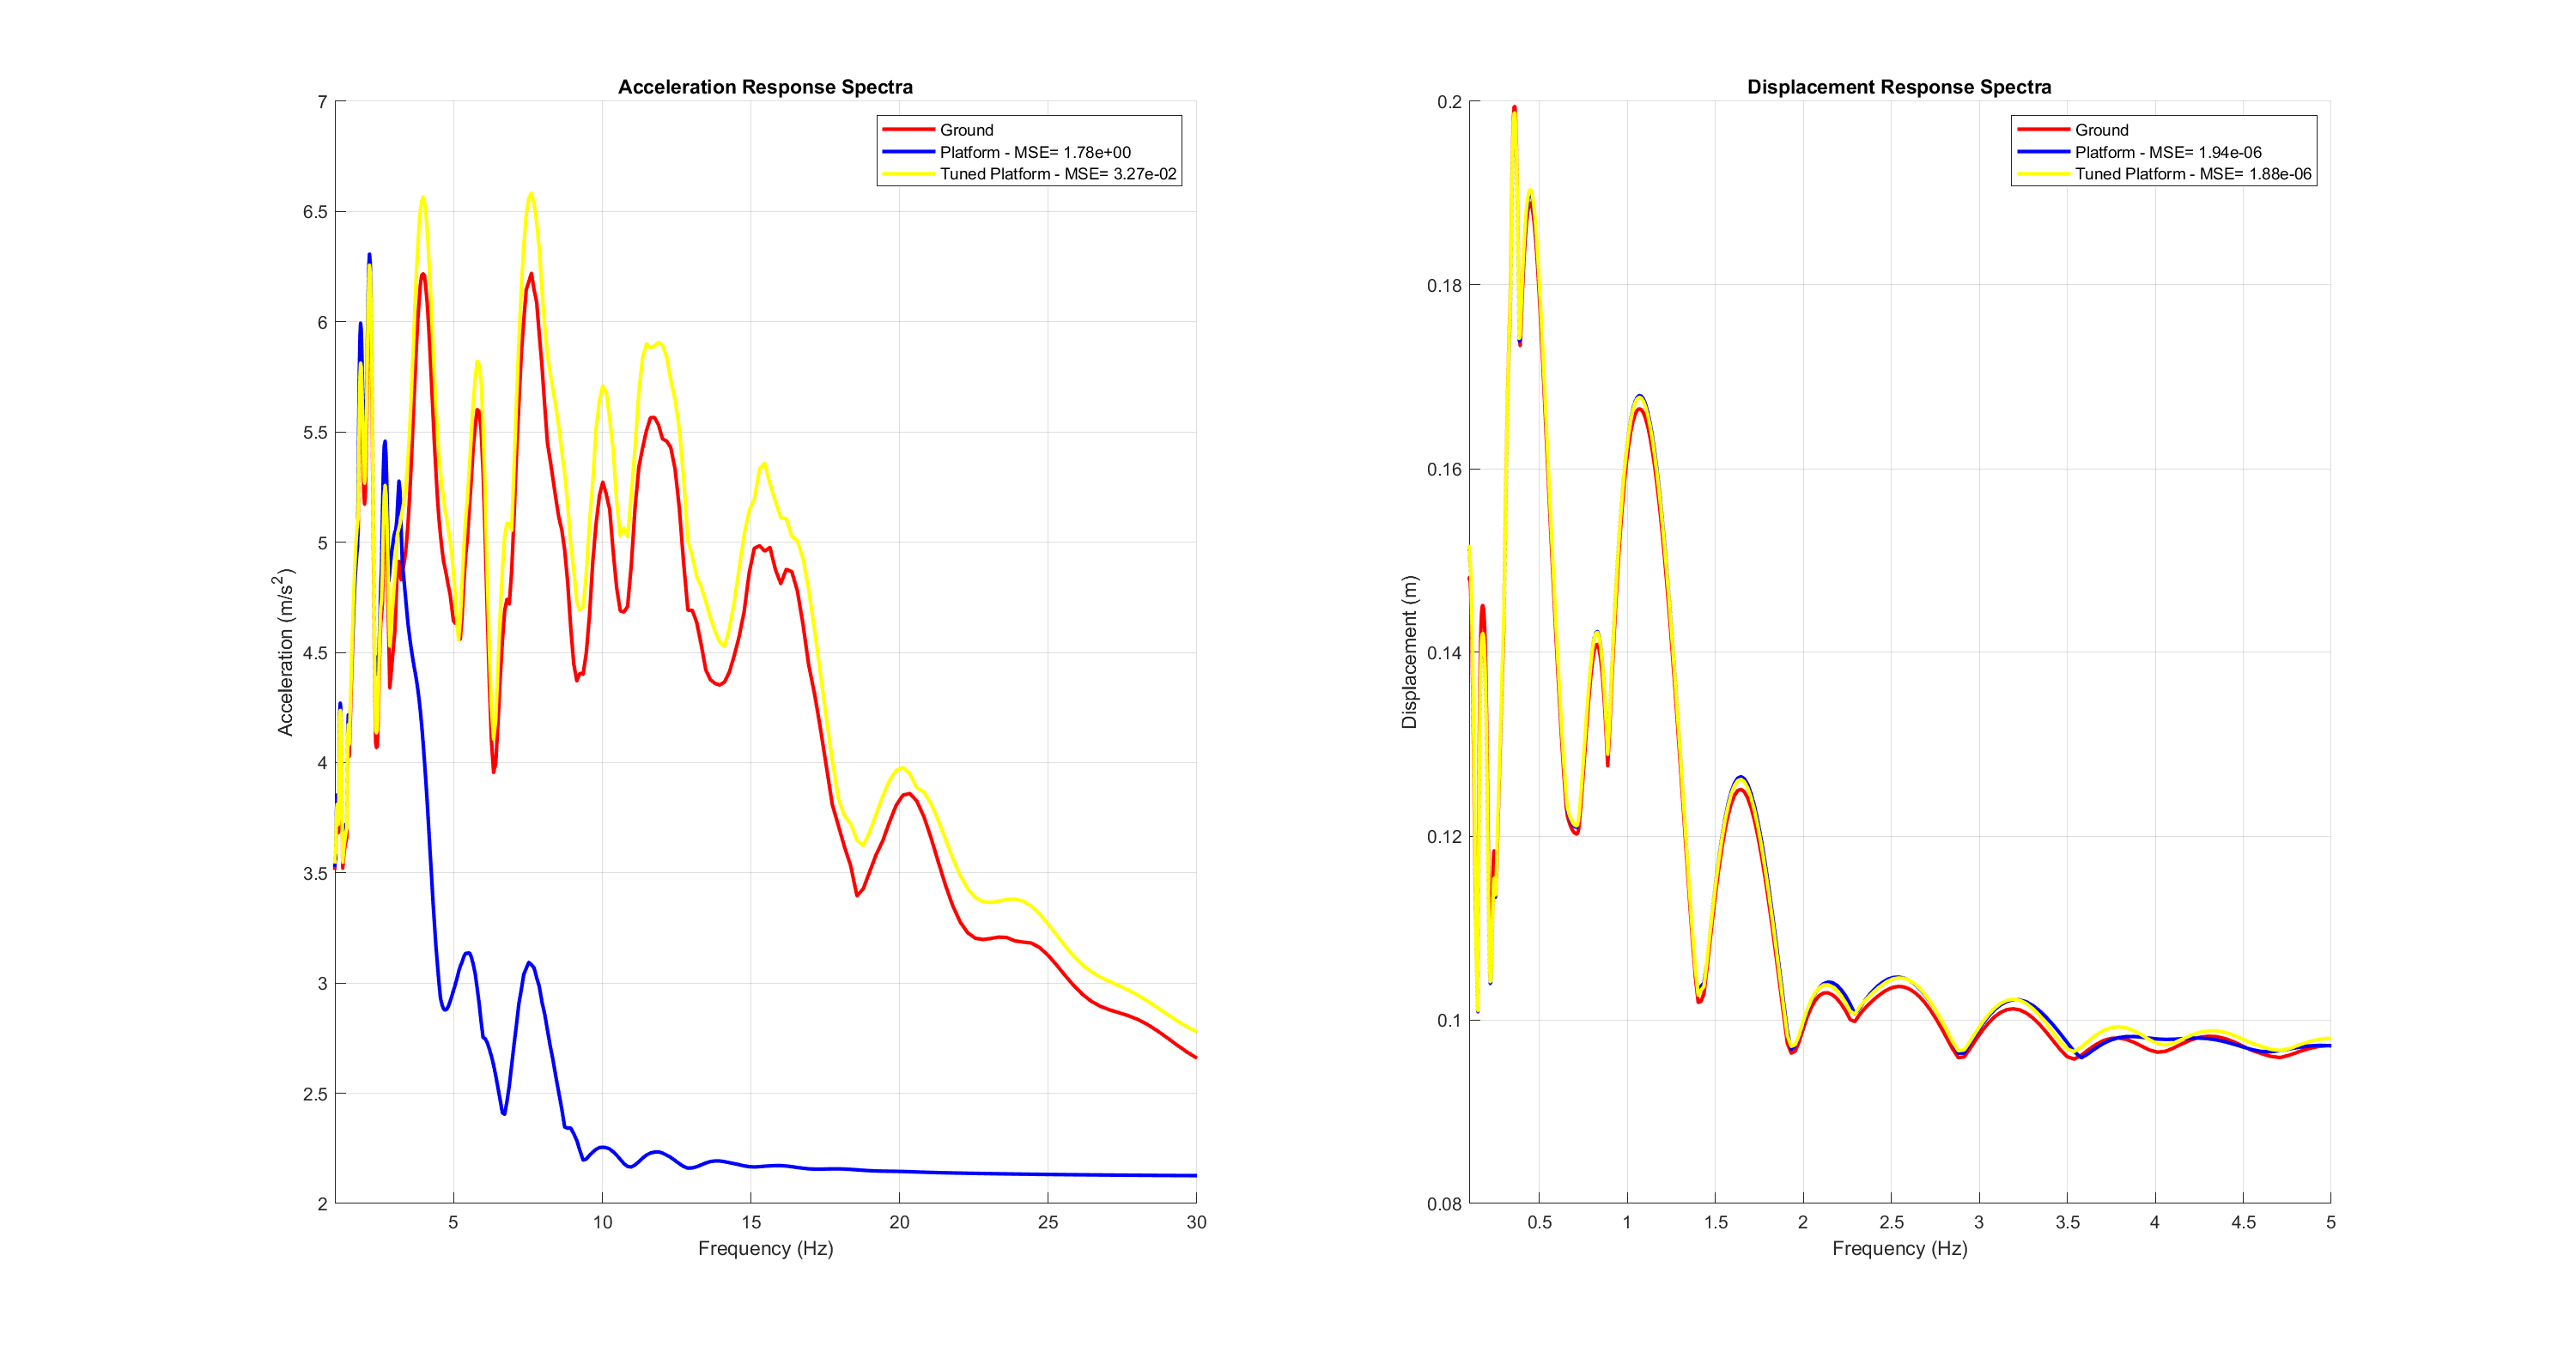
\includegraphics[width=\linewidth]{Sim_Res/Response_Spectra.png}
    \caption{Response spectrum for fault normal signals. The response spectrum was obtained by sampling 500 frequencies, logarithmically spaced between 0.1 and 30 Hz}
    \label{fig_response_spectrum_of_3}
\end{figure}

\begin{table}[h]
    \centering
    \begin{tabular}{ccc}
        \hline
        MSE & F. Parallel  \\
        \hline
        Acceleration & 1.78  \\
        Acceleration (tuned) & 0.0327 \\
        \hline
        Displacement          & $1.94\cdot 10^{-6}$  \\
        Displacement (tuned)  & $1.88 \cdot 10^{-6}$  \\
        \hline
    \end{tabular}
    \caption{Mean squared error for response spectrum of platen with ground response spectrum as baseline }
    \label{tab:mse_rs}
\end{table}

In figures \ref{fig_Platen_Acceleration} to \ref{fig_Platen_Displacement_zoom}, label "MSE" refers to the  respective mean squared error when using the standard controller, and "Tuned MSE" refers to the respective mean squared error when using the tuned PIDF controller.

The acceleration response spectrum mean squared error for the tuned platform is significantly reduced compared to the standard tune (Table \ref{tab:mse_rs}), however, it exceeds the desired response spectrum for the entire frequency spectrum.




\begin{figure}[H]
\begin{minipage}{0.49\textwidth}
    \centering
    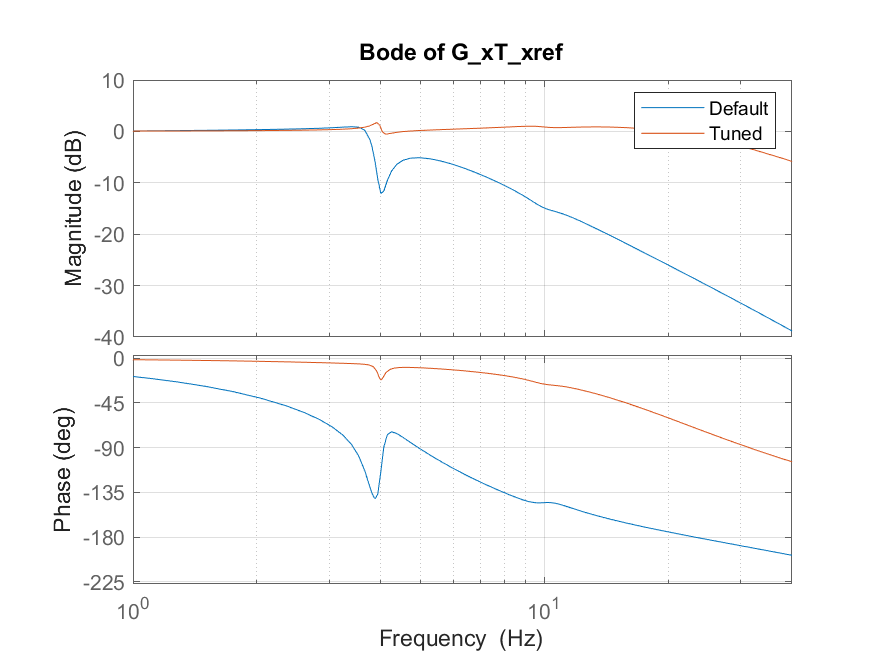
\includegraphics[width=\linewidth]{Sim_Res/Bode_of_G_xT_xref.png}
    \caption{Bode plots of $G_ {xT/x_{\text{ref}}}(s)$ before and after tuning}
    \label{fig_Bode_of_G_xT_xref}    
\end{minipage}
\hfill
\begin{minipage}{0.49\textwidth}
    \centering
    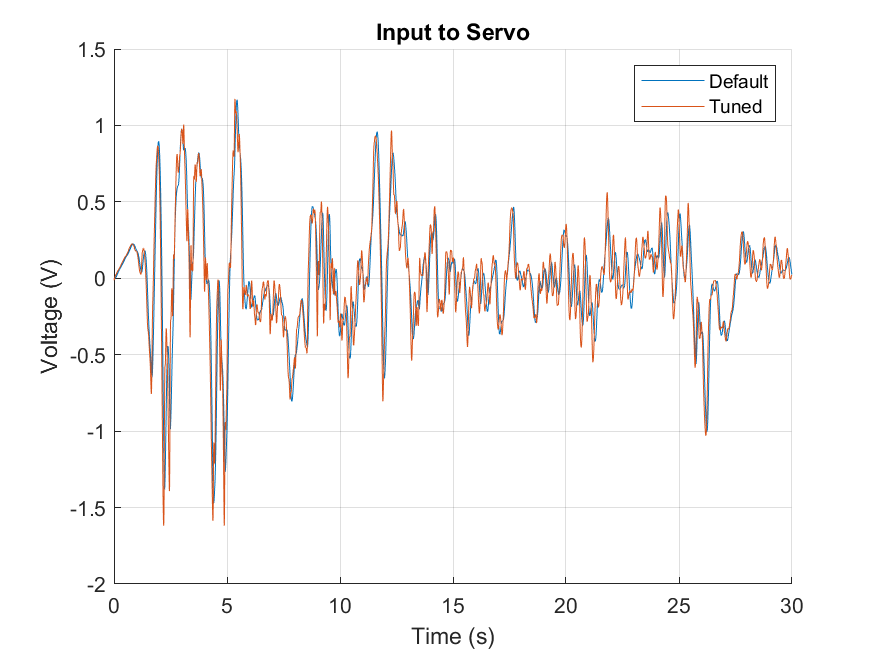
\includegraphics[width=\linewidth]{Sim_Res/Input_to_Servo.png}
    \caption{Input to servo before and after tuning}
    \label{fig_Input_to_Servo}
\end{minipage}
\end{figure}


\begin{figure}[H]
\begin{minipage}{0.49\textwidth}
    \centering
    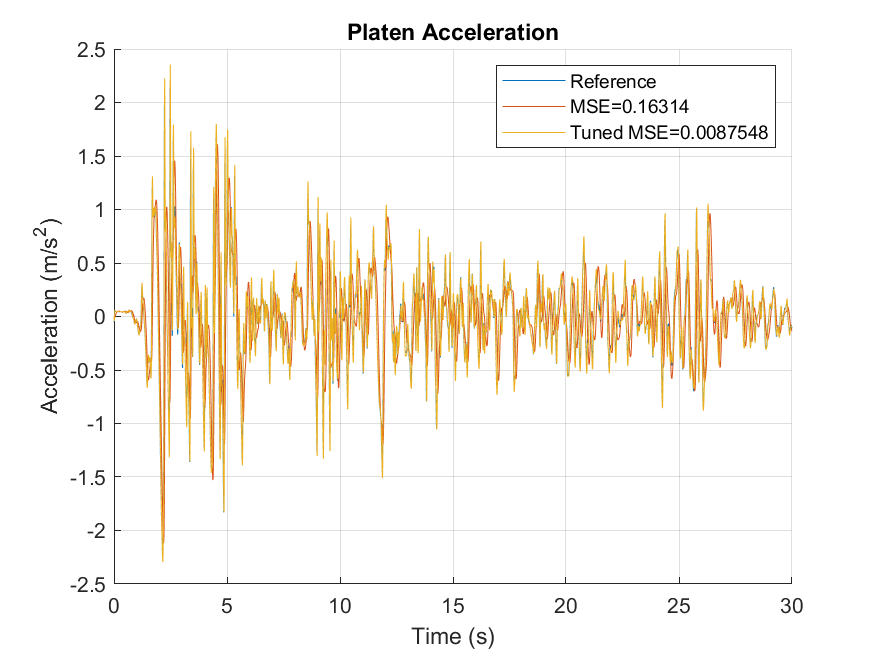
\includegraphics[width=\linewidth]{Sim_Res/Platen_Acceleration.png}
    \caption{Accelerations before and after tuning}
    \label{fig_Platen_Acceleration}
\end{minipage}
\hfill
\begin{minipage}{0.49\textwidth}
    \centering
    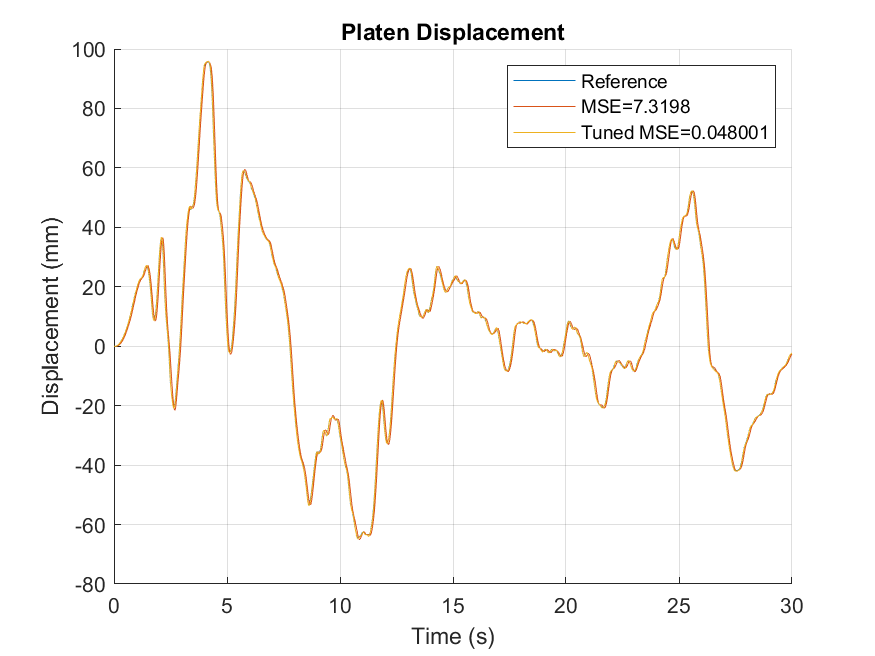
\includegraphics[width=\linewidth]{Sim_Res/Platen_Displacement.png}
    \caption{Displacements before and after tuning}
    \label{fig_Platen_Displacement}
\end{minipage}
\end{figure}

\begin{figure}[H]
\begin{minipage}{0.49\textwidth}
    \centering
    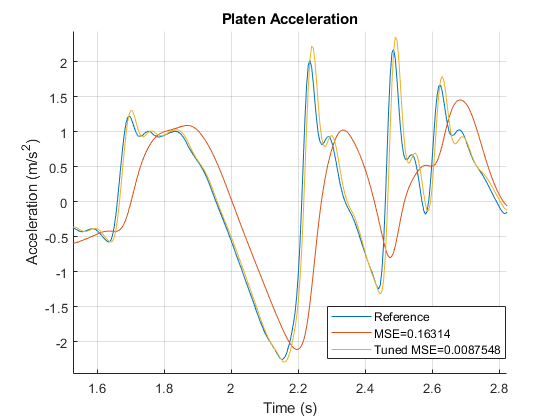
\includegraphics[width=\linewidth]{Sim_Res/Platen_Acceleration_zoom.png}
    \caption{Accelerations before and after tuning - Detailed view of the signals covering the period between 1.5 and 2.7 seconds}
    \label{fig_Platen_Acceleration_zoom}
\end{minipage}
\hfill
\begin{minipage}{0.49\textwidth}
    \centering
    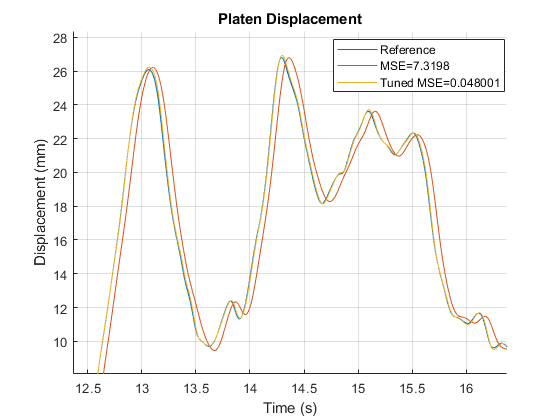
\includegraphics[width=\linewidth]{Sim_Res/Platen_Displacement_zoom.png}
    \caption{Displacements before and after tuning - Detailed view of the signals covering the period between 14.1 and 15.7 seconds}
    \label{fig_Platen_Displacement_zoom}
\end{minipage}
\end{figure}

\begin{figure}[H]
\begin{minipage}{0.49\textwidth}
    \centering
    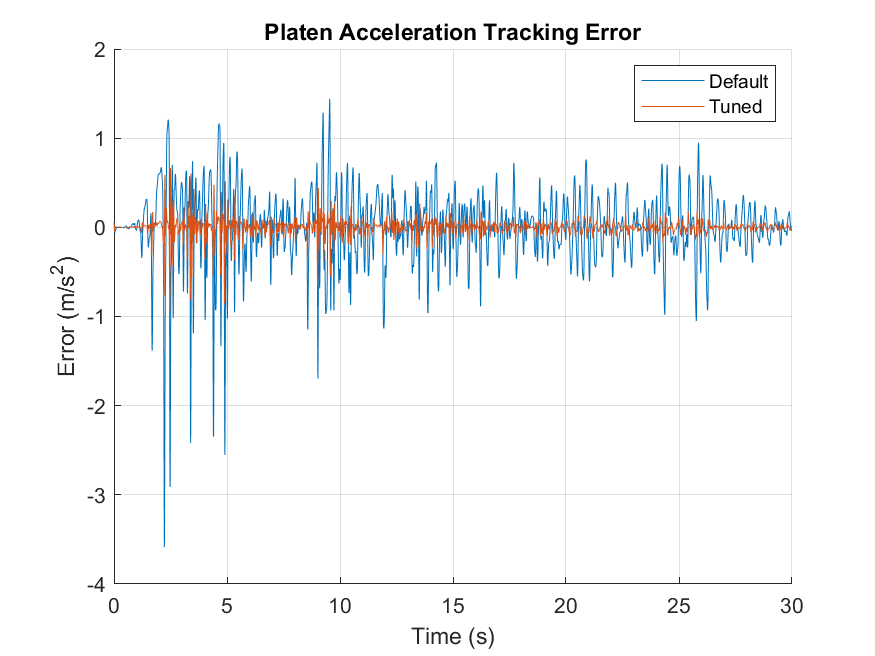
\includegraphics[width=\linewidth]{Sim_Res/Platen_Acceleration_Tracking_Error.png}
    \caption{Acceleration tracking error before and after tuning}
    \label{fig_Platen_Acceleration_Tracking_Error}
\end{minipage}
\hfill
\begin{minipage}{0.49\textwidth}
    \centering
    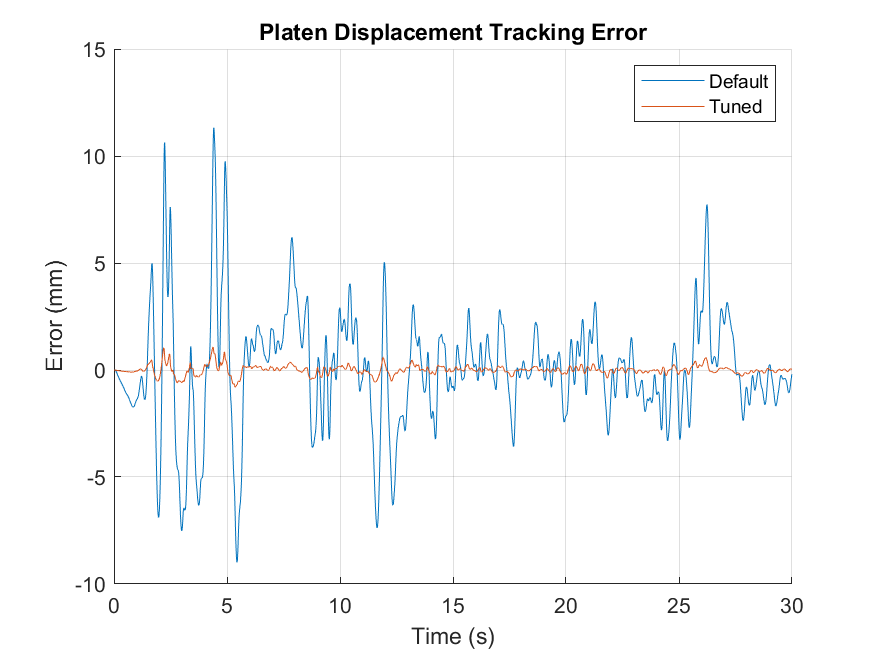
\includegraphics[width=\linewidth]{Sim_Res/Platen_Displacement_Tracking_Error.png}
    \caption{Displacement tracking error before and after tuning}
    \label{fig_Platen_Displacement_Tracking_Error}
\end{minipage}
\end{figure}

\subsubsection{Performance Sensitivity to Test Structure Parameters}%Analysis of Tuned PIDF 

The mass, modal frequencies, and damping of the structures coupled to the seismic table have an impact on how well it is able to track the reference. In this section, we will analyse how the seismic table with the tuned PIDF performs for different damping, modal frequencies, and mass of the test structure. 

The legend of figures \ref{Resp_Spectre_low_high_freq_and_damp} through to \ref{Resp_Spectre_f1_2415}, shows the modal properties of the structure on test, the maximum absolute values of the input to the servo-valve $i_{sv}$ (in volts) and force applied by the actuator (in kilo newtons), and the mean square error for the respective response spectrum.

\begin{figure}[H]
    \centering
    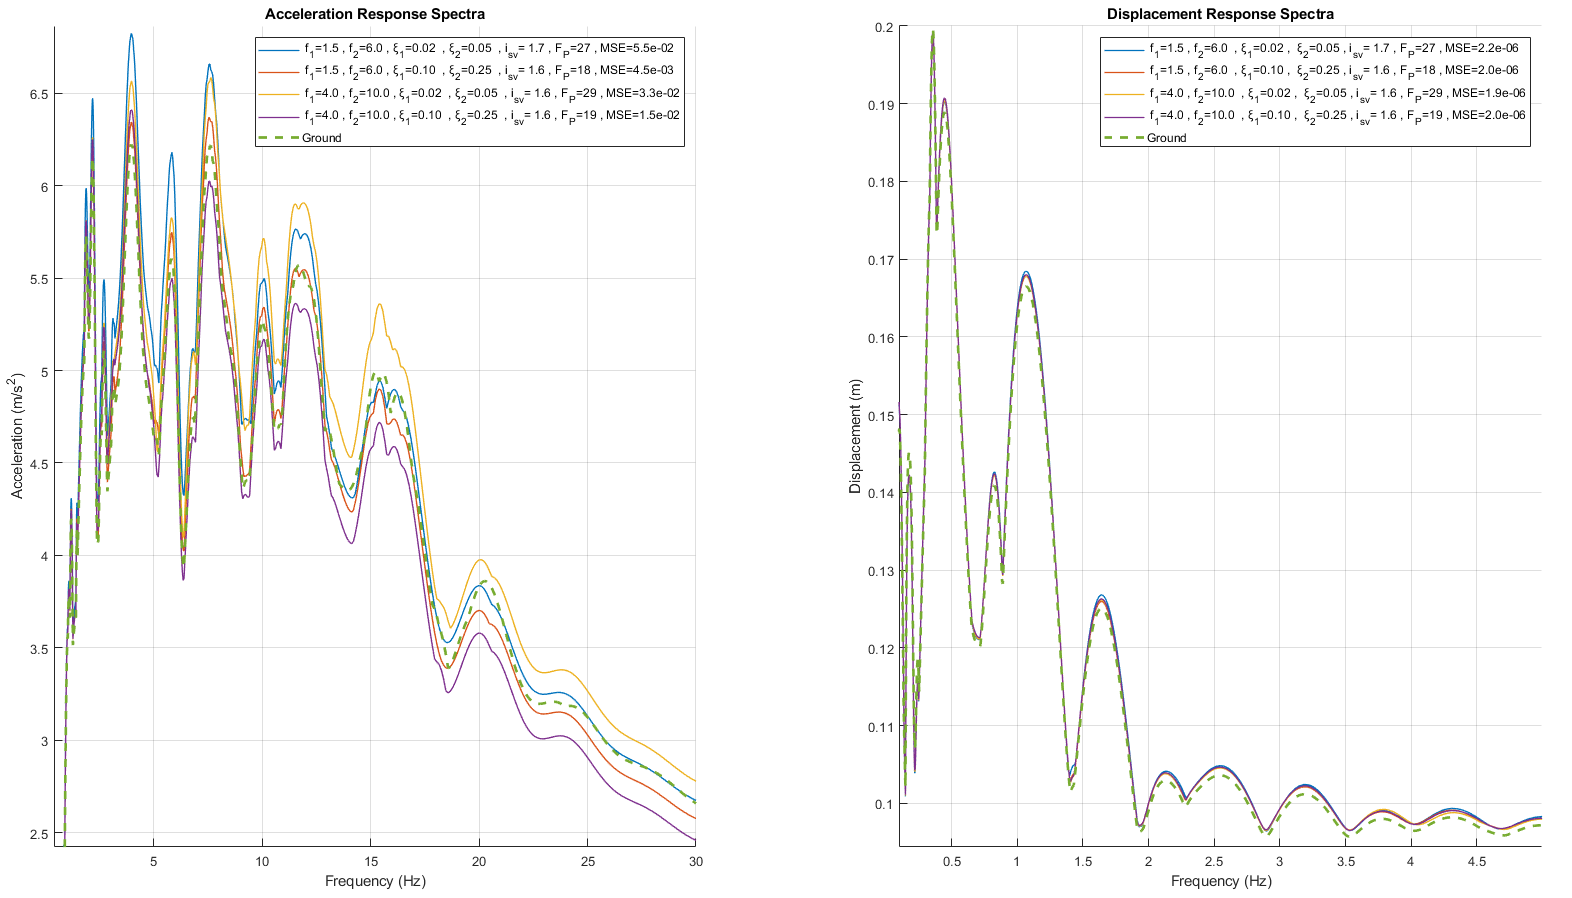
\includegraphics[width=1\linewidth]{MSE_Resp_Spectre/Resp_Spectre_low_high_freq_and_damp_cut.png}
    \caption{Response spectra for $m_1=m_2=2 \text{ ton}$, and different modal frequencies and damping}
    \label{Resp_Spectre_low_high_freq_and_damp}
\end{figure}

\begin{figure}[H]
    \centering
    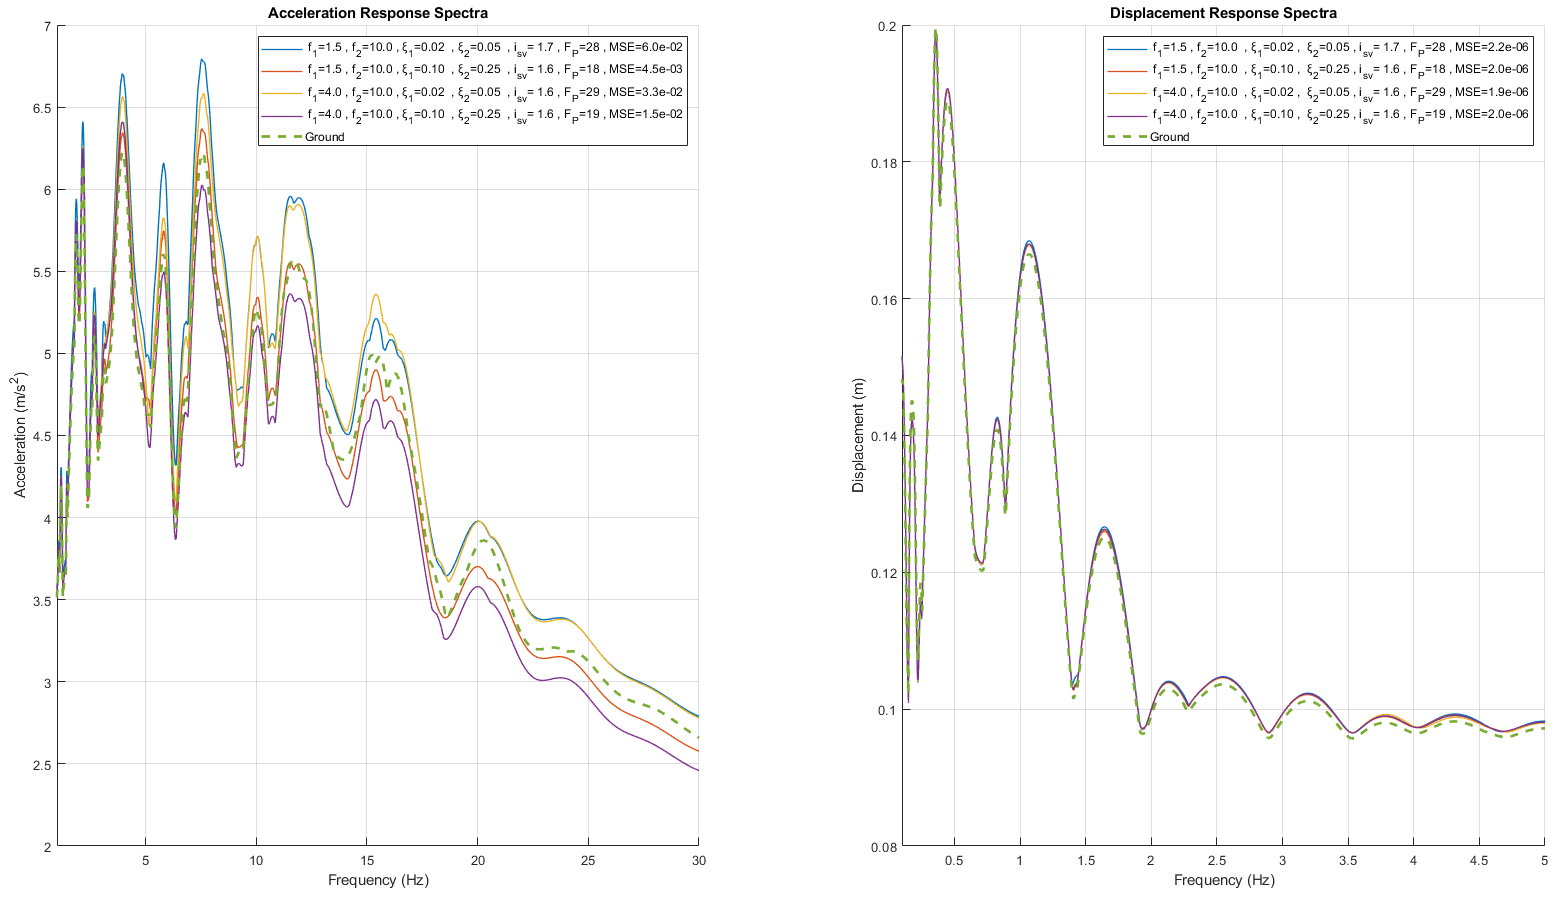
\includegraphics[width=1\linewidth]{MSE_Resp_Spectre/Resp_Spectre_f2=10_cut.png}
    \caption{Response spectra for $m_1=m_2=2\text{ ton}$, with $f_2=10$ Hz}
    %\label{}
\end{figure}

\begin{figure}[H]
    \centering
    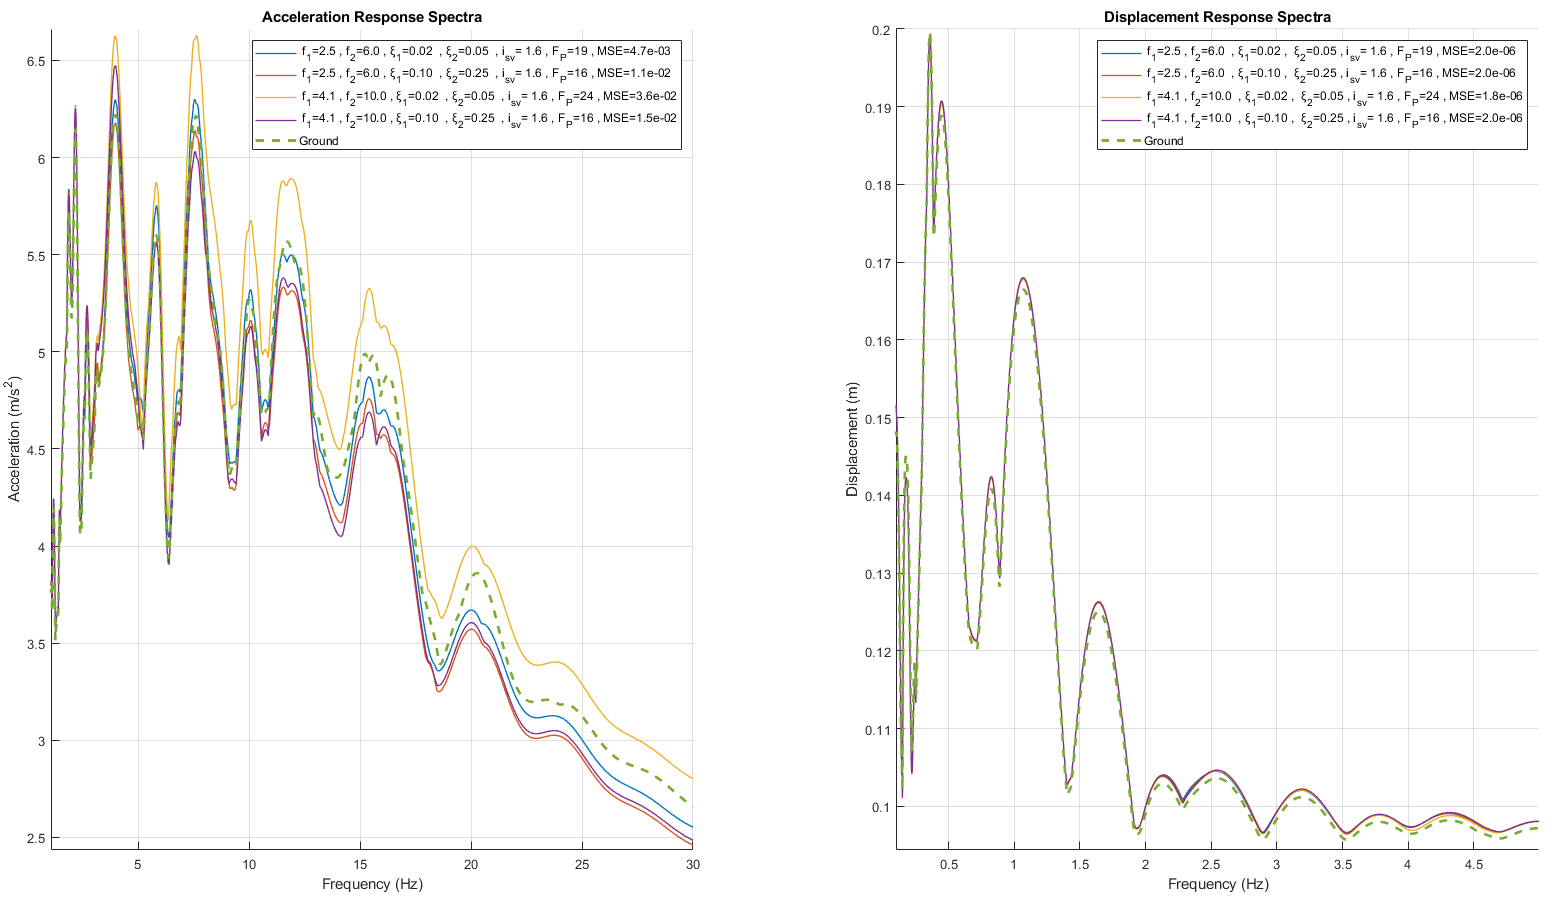
\includegraphics[width=1\linewidth]{MSE_Resp_Spectre/Resp_Spectre_f1_2415_cut.png}
    \caption{Response spectra for $m_1=m_2=2\text{ ton}$, and modal frequencies which are close together ($f_2 \approx2.415\cdot f_1$) (see figure \ref{fig_close_modal_freqs})}
    \label{Resp_Spectre_f1_2415}
\end{figure}



\begin{figure}[H]
    \centering
    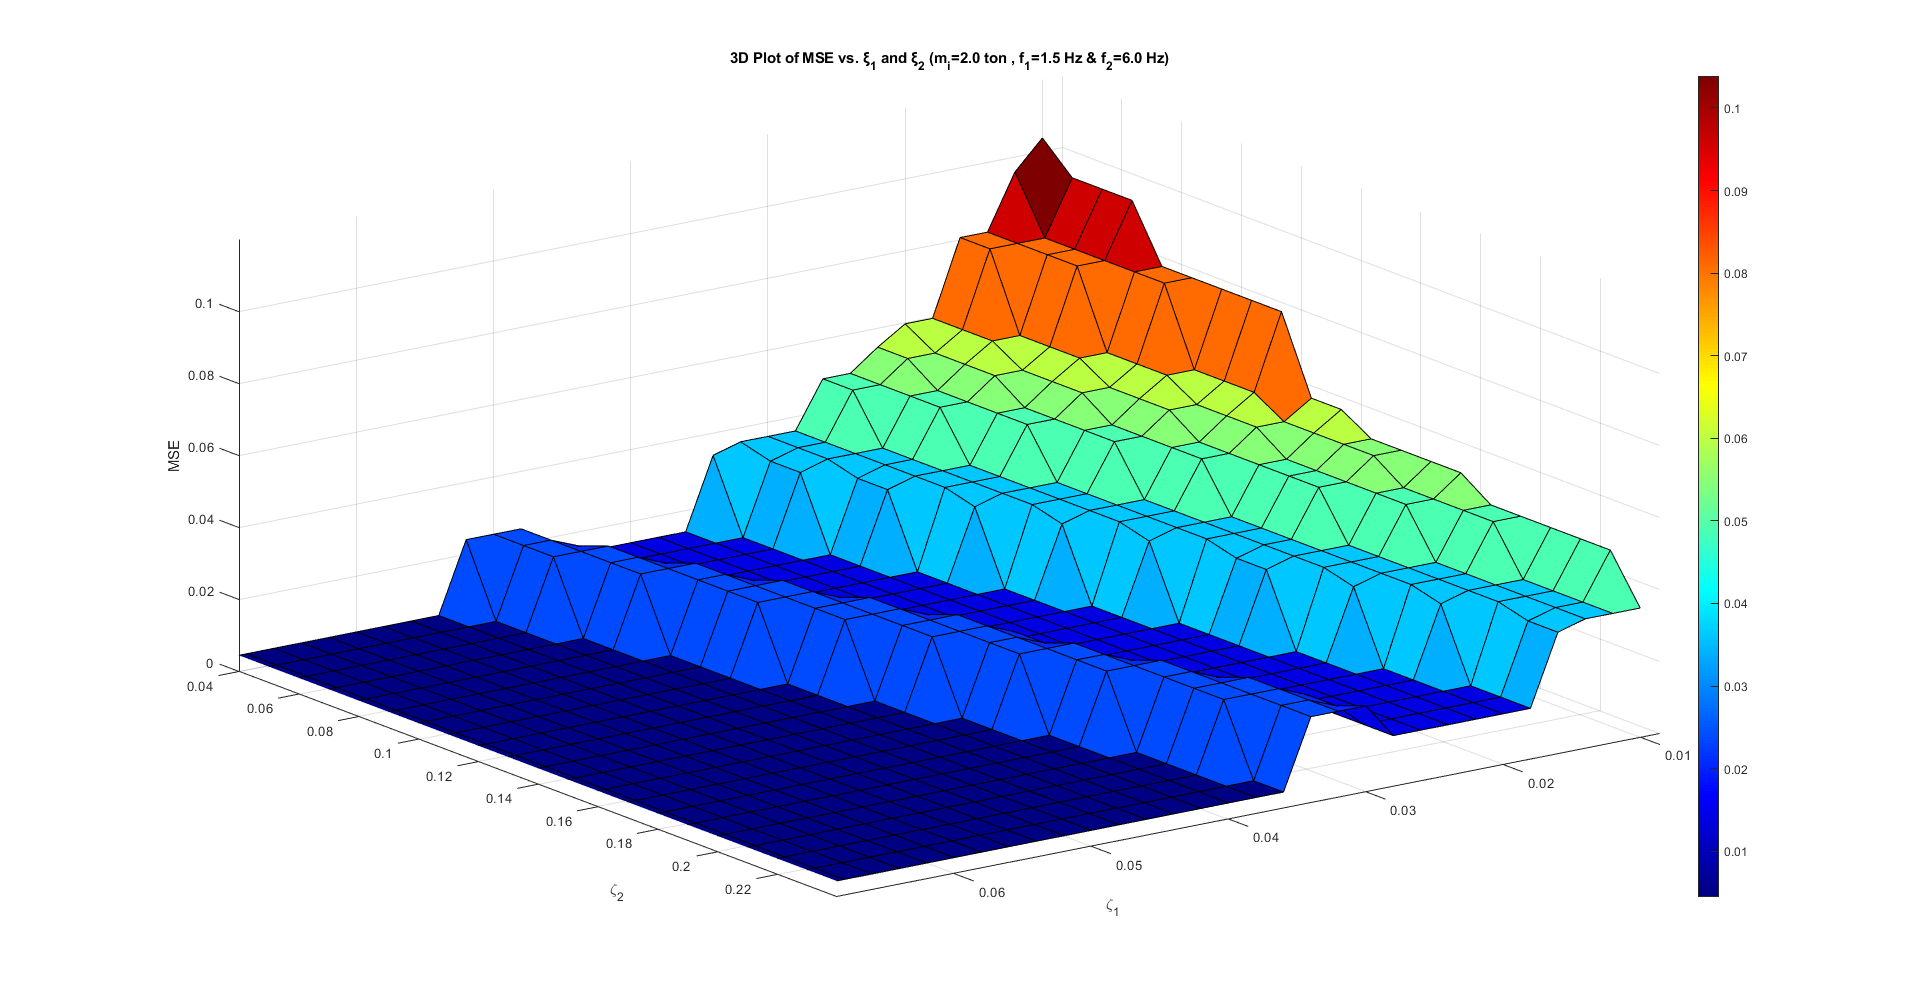
\includegraphics[width=1\linewidth]{MSE_Zeta/Surf_Zeta_LowFreq_IsoView.png}
    \caption{Response Spectra MSE vs $\zeta_1$ and $\zeta_2$, with $m_1=m_2=2\text{ ton, }f_1=1.5 Hz, f_2=6 Hz$}
    %\label{}
\end{figure}


\begin{figure}[H]
\begin{minipage}{0.45\textwidth}
    \centering
    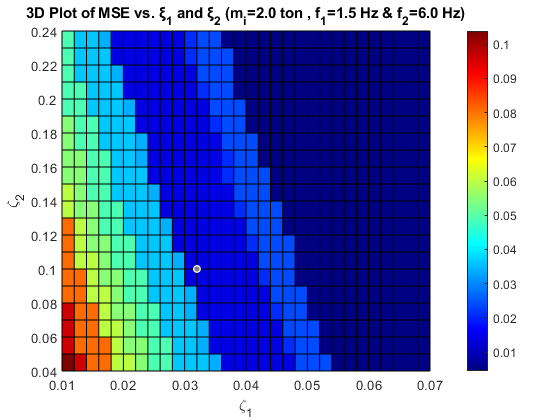
\includegraphics[width=\linewidth]{MSE_Zeta/Surf_Zeta_LowFreq_TopView.png}
    \caption{Response Spectra MSE vs $\zeta_1$ and $\zeta_2$, with $m_1=m_2=2\text{ ton, }f_1=1.5 Hz, f_2=6 Hz$}
    %\label{}
\end{minipage}
\hfill
\begin{minipage}{0.45\textwidth}
    \centering
    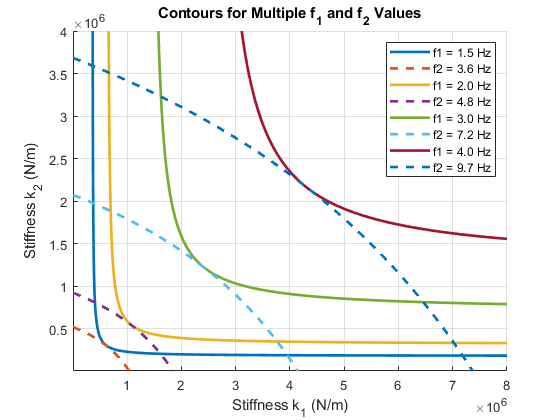
\includegraphics[width=\linewidth]{PID_MSE/stiffness_solutions.png}
    \caption{For the 2DOF model (fig.\ref{schematic_2dof}), the modal frequency $f_2$ must be greater than $2.415 \times f_1$  (Equation \ref{eq_modal_frequencies})}
    \label{fig_close_modal_freqs}
\end{minipage}
\end{figure}

\begin{figure}[H]
\begin{minipage}{0.45\textwidth}
    \centering
    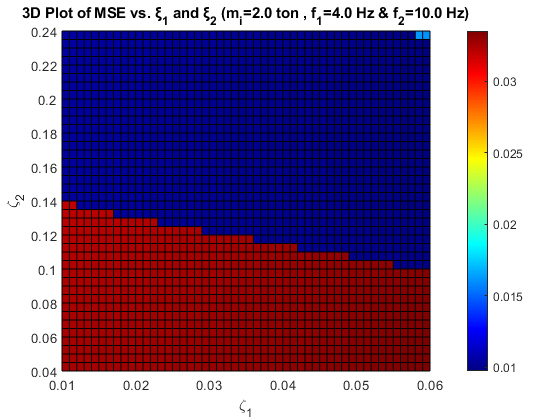
\includegraphics[width=\linewidth]{MSE_Zeta/MSE vs Zeta (m_i=2.0,f_1=4.0, f_2=10.0)_old.png}
    \caption{Response Spectra MSE vs $\zeta_1$ and $\zeta_2$, with $m_1=m_2=2\text{ ton, }f_1=4 Hz, f_2=10 Hz$. For high modal frequencies, the response spectrum MSE increases abruptly for $\zeta_2 > 0.14 - 0.8\cdot \zeta_1 $, but remains mostly unchanged otherwise.}
    %\label{fig:enter-label}
\end{minipage}
\hfill
\begin{minipage}{0.45\textwidth}
    \centering
    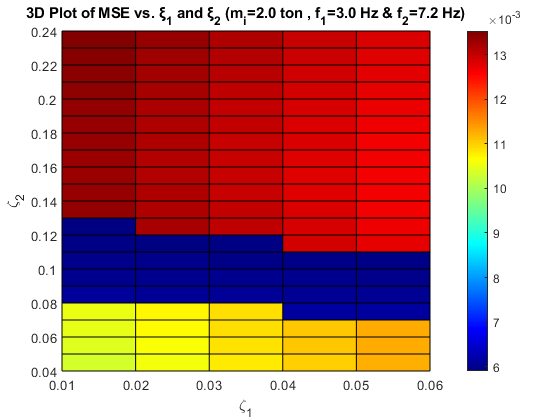
\includegraphics[width=1\linewidth]{MSE_Zeta/MSE vs Zeta (m_i=2.0,f_1=3.0, f_2=7.2).png}
    \caption{Response Spectra MSE vs $\zeta_1$ and $\zeta_2$, with $m_1=m_2=2\text{ ton, }f_1=3 Hz, f_2=7.2 Hz$ (modal frequencies close together)}
    %\label{fig:enter-label}
\end{minipage}
\end{figure}


\begin{figure}[H]
    \centering
    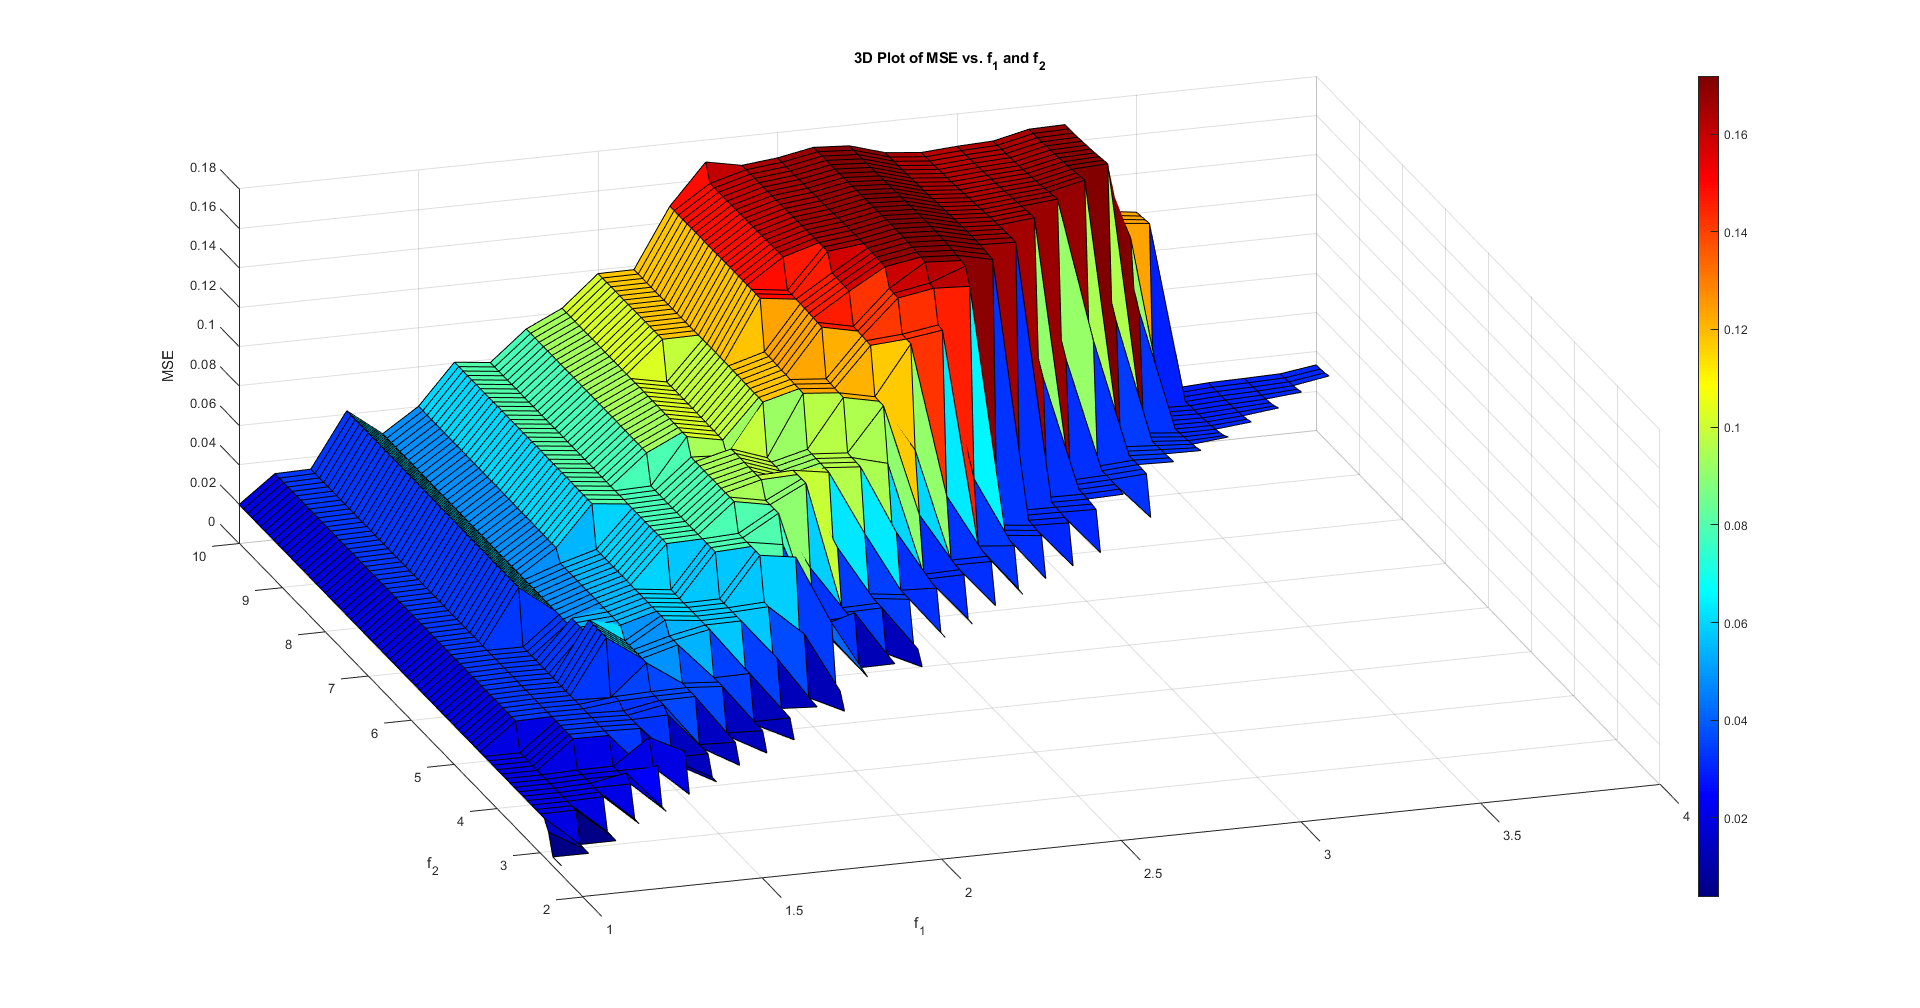
\includegraphics[width=1\linewidth]{PID_MSE/PID_MSE_Surface_frequency_blue_red_isoview_lowDamp.png}
    \caption{Response Spectra MSE vs $f_1$ and $f_2$, with $m_1=m_2=2\text{ ton, } \zeta_1=0.02, \zeta_2=0.05$ (low damping)}
    %\label{}
\end{figure}


\begin{figure}[H]
\begin{minipage}{0.44\textwidth}
    \centering
    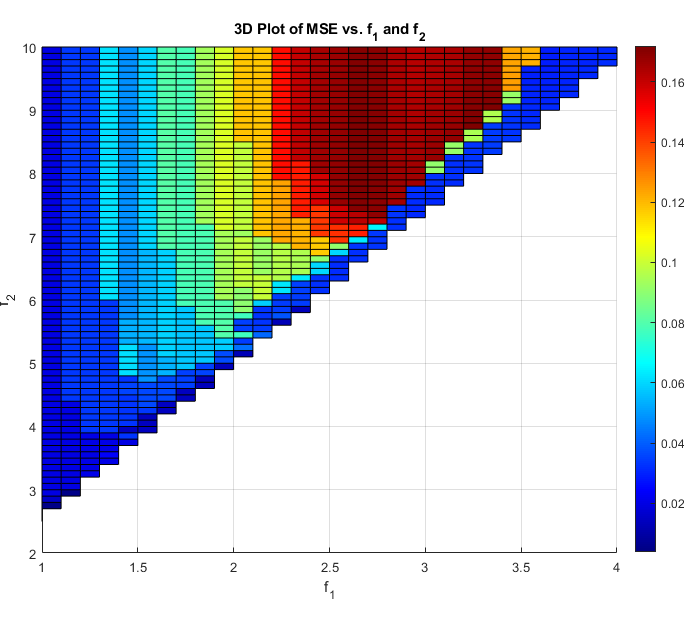
\includegraphics[width=1\linewidth]{PID_MSE/PID_MSE_Surface_frequency_blue_red_topview_lowDamp.png}
    \caption{Response Spectra MSE vs $f_1$ and $f_2$, with $m_1=m_2=2\text{ ton, } \zeta_1=0.02, \zeta_2=0.05$ (low damping)}
    %\label{}
\end{minipage}
\hfill
\begin{minipage}{0.45\textwidth}
    \centering
    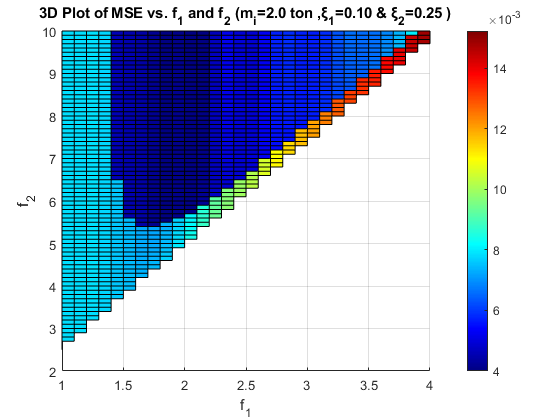
\includegraphics[width=1\linewidth]{MSE_Freq/MSE vs Freq (m_i=2.0,zeta1=0.10,zeta2=0.25)_topview.png}
    \caption{Response Spectra MSE vs $f_1$ and $f_2$, with $m_1=m_2=2\text{ ton, } \zeta_1=0.1, \zeta_2=0.25$ (high damping)}
    %\label{}
\end{minipage}
\end{figure}



Structures with % higher modal frequencies ($f_1=4$ Hz \& $f_2=10$ Hz) and 
lower damping ($\zeta_1=0.02$ \& $\zeta_2=0.05$) result in response spectra which exceeds the desired one over the entire frequency spectrum, while structures with higher damping ($\zeta_1=0.1$ \& $\zeta_2=0.25$) result in response spectra which fall short of the desired one.

The affect of modal frequencies on the performance of the seismic table is unclear, and likely depends heavily on the frequency content of the seismic signal.


\clearpage
\subsection{Optimal Control}  

\subsubsection{ State Space Model } \label{section_ss_model}
For the 2-DoF system coupled to the seismic table, the following state space model was derived, where:

\begin{align}
    \dot{x}(t) \enspace &=  \quad A \cdot x(t) \ + \ B \cdot u(t) \ \Longleftrightarrow \nonumber \\
    \Longleftrightarrow 
    \begin{bmatrix} 
        \dot{Q}_{sv} \\[6pt]
        \dot{F}_p \\[6pt]
        \dot{x}_T \\[6pt]
        \dot{x}_1 \\[6pt]
        \dot{x}_2 \\[6pt]
        \ddot{x}_T \\[6pt]
        \ddot{x}_1 \\[6pt]
        \ddot{x}_2 
    \end{bmatrix} &=
    \begin{bmatrix}
    \frac{-1}{\tau_{sv}} &  0 & 0 & 0 & 0 & 0 & 0 & 0 & 0\\[6pt]
    \frac{k_h}{A}  & \frac{- k_h k_{pl}}{A^2} & 0              & 0 & 0                & 0   & -k_h & 0               & 0 \\[6pt]
                    0 &               0              & 0 & 0                & 0   & 1    & 0               & 0 \\[6pt]
                    0 &               0              & 0 & 0                & 0   & 0    & 1               & 0 \\[6pt]
                    0 &               0              & 0 & 0                & 0   & 0    & 0               & 1 \\[6pt]
                    0 &                \frac{1}{m_T} & \frac{-k_1}{m_T} & \frac{k_1}{m_T}     &  0              & \frac{-c_T - c_1 }{m_T} & \frac{ c_1 }{m_T}   & 0               \\[6pt]
                    0 &                0             & \frac{k_1}{m_1}  &\frac{-k_1-k_2}{m_1} & \frac{k_2}{m_1} & \frac{c_1}{m_1}         &\frac{-c_1-c_2}{m_1} & \frac{c_2}{m_1} \\[6pt]
                    0 &                0             &         0        & \frac{k_2}{m_2}     & \frac{-k_2}{m_2}& 0                       & \frac{c_2}{m_2}     & \frac{-c_2}{m_2}
    \end{bmatrix}             
    \begin{bmatrix}
        Q_{sv} \\[6pt]
        F_p \\[6pt]
        x_T \\[6pt]
        x_1 \\[6pt]
        x_2 \\[6pt]
        \dot{x}_T \\[6pt]
        \dot{x}_1 \\[6pt]
        \dot{x}_2
    \end{bmatrix} +
    \begin{bmatrix}
        \frac{k_{sv}k_q}{\tau_{sv}}  \\[6pt]
        0 \\[6pt]
        0 \\[6pt]
        0 \\[6pt]
        0 \\[6pt]
        0 \\[6pt]
        0 \\[6pt]
        0
    \end{bmatrix}
    \cdot i_{sv}
\end{align}

\vspace{2mm}

Where the desired output is $x_T$, and there is no feedthrough: 
$$ C = \begin{bmatrix}
0 & 0 & 1 & 0 & 0 & 0 & 0 & 0
\end{bmatrix}
\quad \quad D = 0$$
\begin{equation}
y(t) = C\cdot x(t) + D\cdot u(t) = x_T
\end{equation}

\subsubsection{Controllability \& Observability}
Controllability and observability matrices were built in MATLAB with \emph{ctrb} and \emph{obsv} commands while using variable precision arithmetic to evaluate each element to ten thousand significant digits, and were verified to be of full rank.


\subsubsection{LQR Servo Controller}



\begin{figure}[H]
\begin{minipage}{0.49\textwidth}
For the tracking loop shown in figure \ref{fig_LQI_loop}, where \emph{sys} is the state space model presented in section \ref{section_ss_model}, the optimal state feedback control law which minimizes the cost function (equation \ref{eq_LQI_cost_function}) was computed using MATLAB \emph{lqi} function, for $R=10^{-9}$ and different $Q$ matrices.

The state weight matrix $Q$ had every element set to zero, except the entry corresponding to the integrated tracking error $x_i$, which as initially set to $10^3$, which resulted in a similar bandwidth to the tuned PIDF(figure \ref{fig_Bode_LQI_Qe3}), and then increased to $10^9$, because this increased the bandwidth, but, unlike the PIDF, did not result in amplification at low frequencies.(Figure \ref{fig_Bode_LQI_Qe9} to \ref{fig_Platen_Displacement_Tracking_Error_LQI_Qe9}).

\end{minipage}
\hfill
\begin{minipage}{0.49\textwidth}
    \centering
    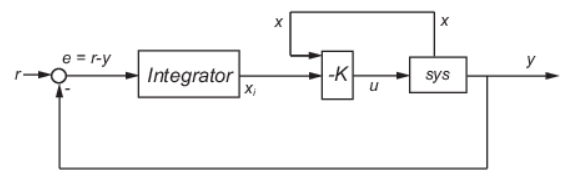
\includegraphics[width=\linewidth]{LQI/LQI_loop.png}
    \caption{Tracking loop with full state feedback control.}
    \label{fig_LQI_loop}

    \begin{equation}
     J(u) = \int ^{\infty}_0 (x^{T}(t)Qx(t) + u^{T}(t)Ru(t)) dt 
     \label{eq_LQI_cost_function}
    \end{equation} 
    \end{minipage}
\end{figure}



    
\begin{figure}[H]
\begin{minipage}{0.49\textwidth}
    \centering
    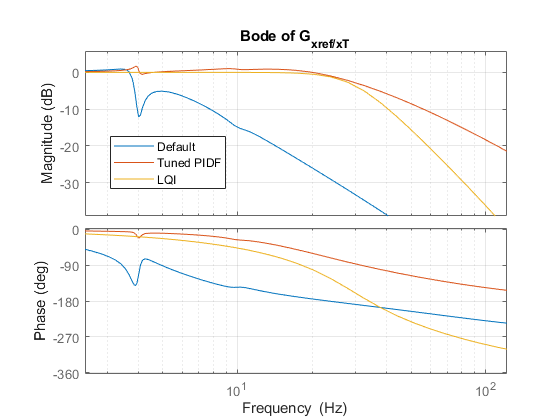
\includegraphics[width=\linewidth]{LQI/Sim_Res_Qe3/Bode_of_G_xT_xref.png}
    \caption{Bode plots of $G_ {xT/x_{\text{ref}}}(s)$ for the default controller, tuned PIDF, and optimal state-feedback controller with $Q=10^3$ (which results in a similar bandwidth to the tuned PIDF).}
    \label{fig_Bode_LQI_Qe3} 
\end{minipage}
\hfill
\begin{minipage}{0.49\textwidth}
    \centering
    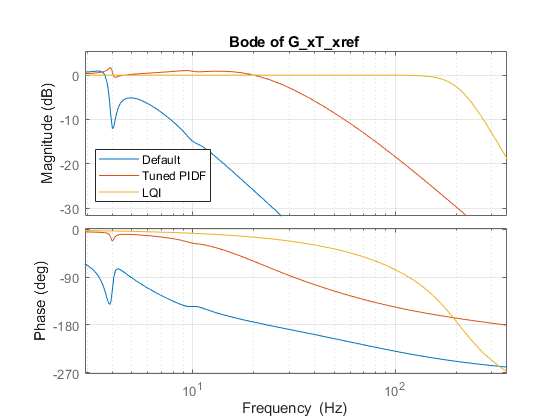
\includegraphics[width=\linewidth]{LQI/Sim_Res_Qe9/Bode_of_G_xT_xref.png}
    \caption{Bode plots of $G_ {xT/x_{\text{ref}}}(s)$ for the default controller, tuned PIDF, and optimal state-feedback controller with $Q=10^9$.}
    \label{fig_Bode_LQI_Qe9}
\end{minipage}
\end{figure}

    

\begin{figure}[H]
    \centering
    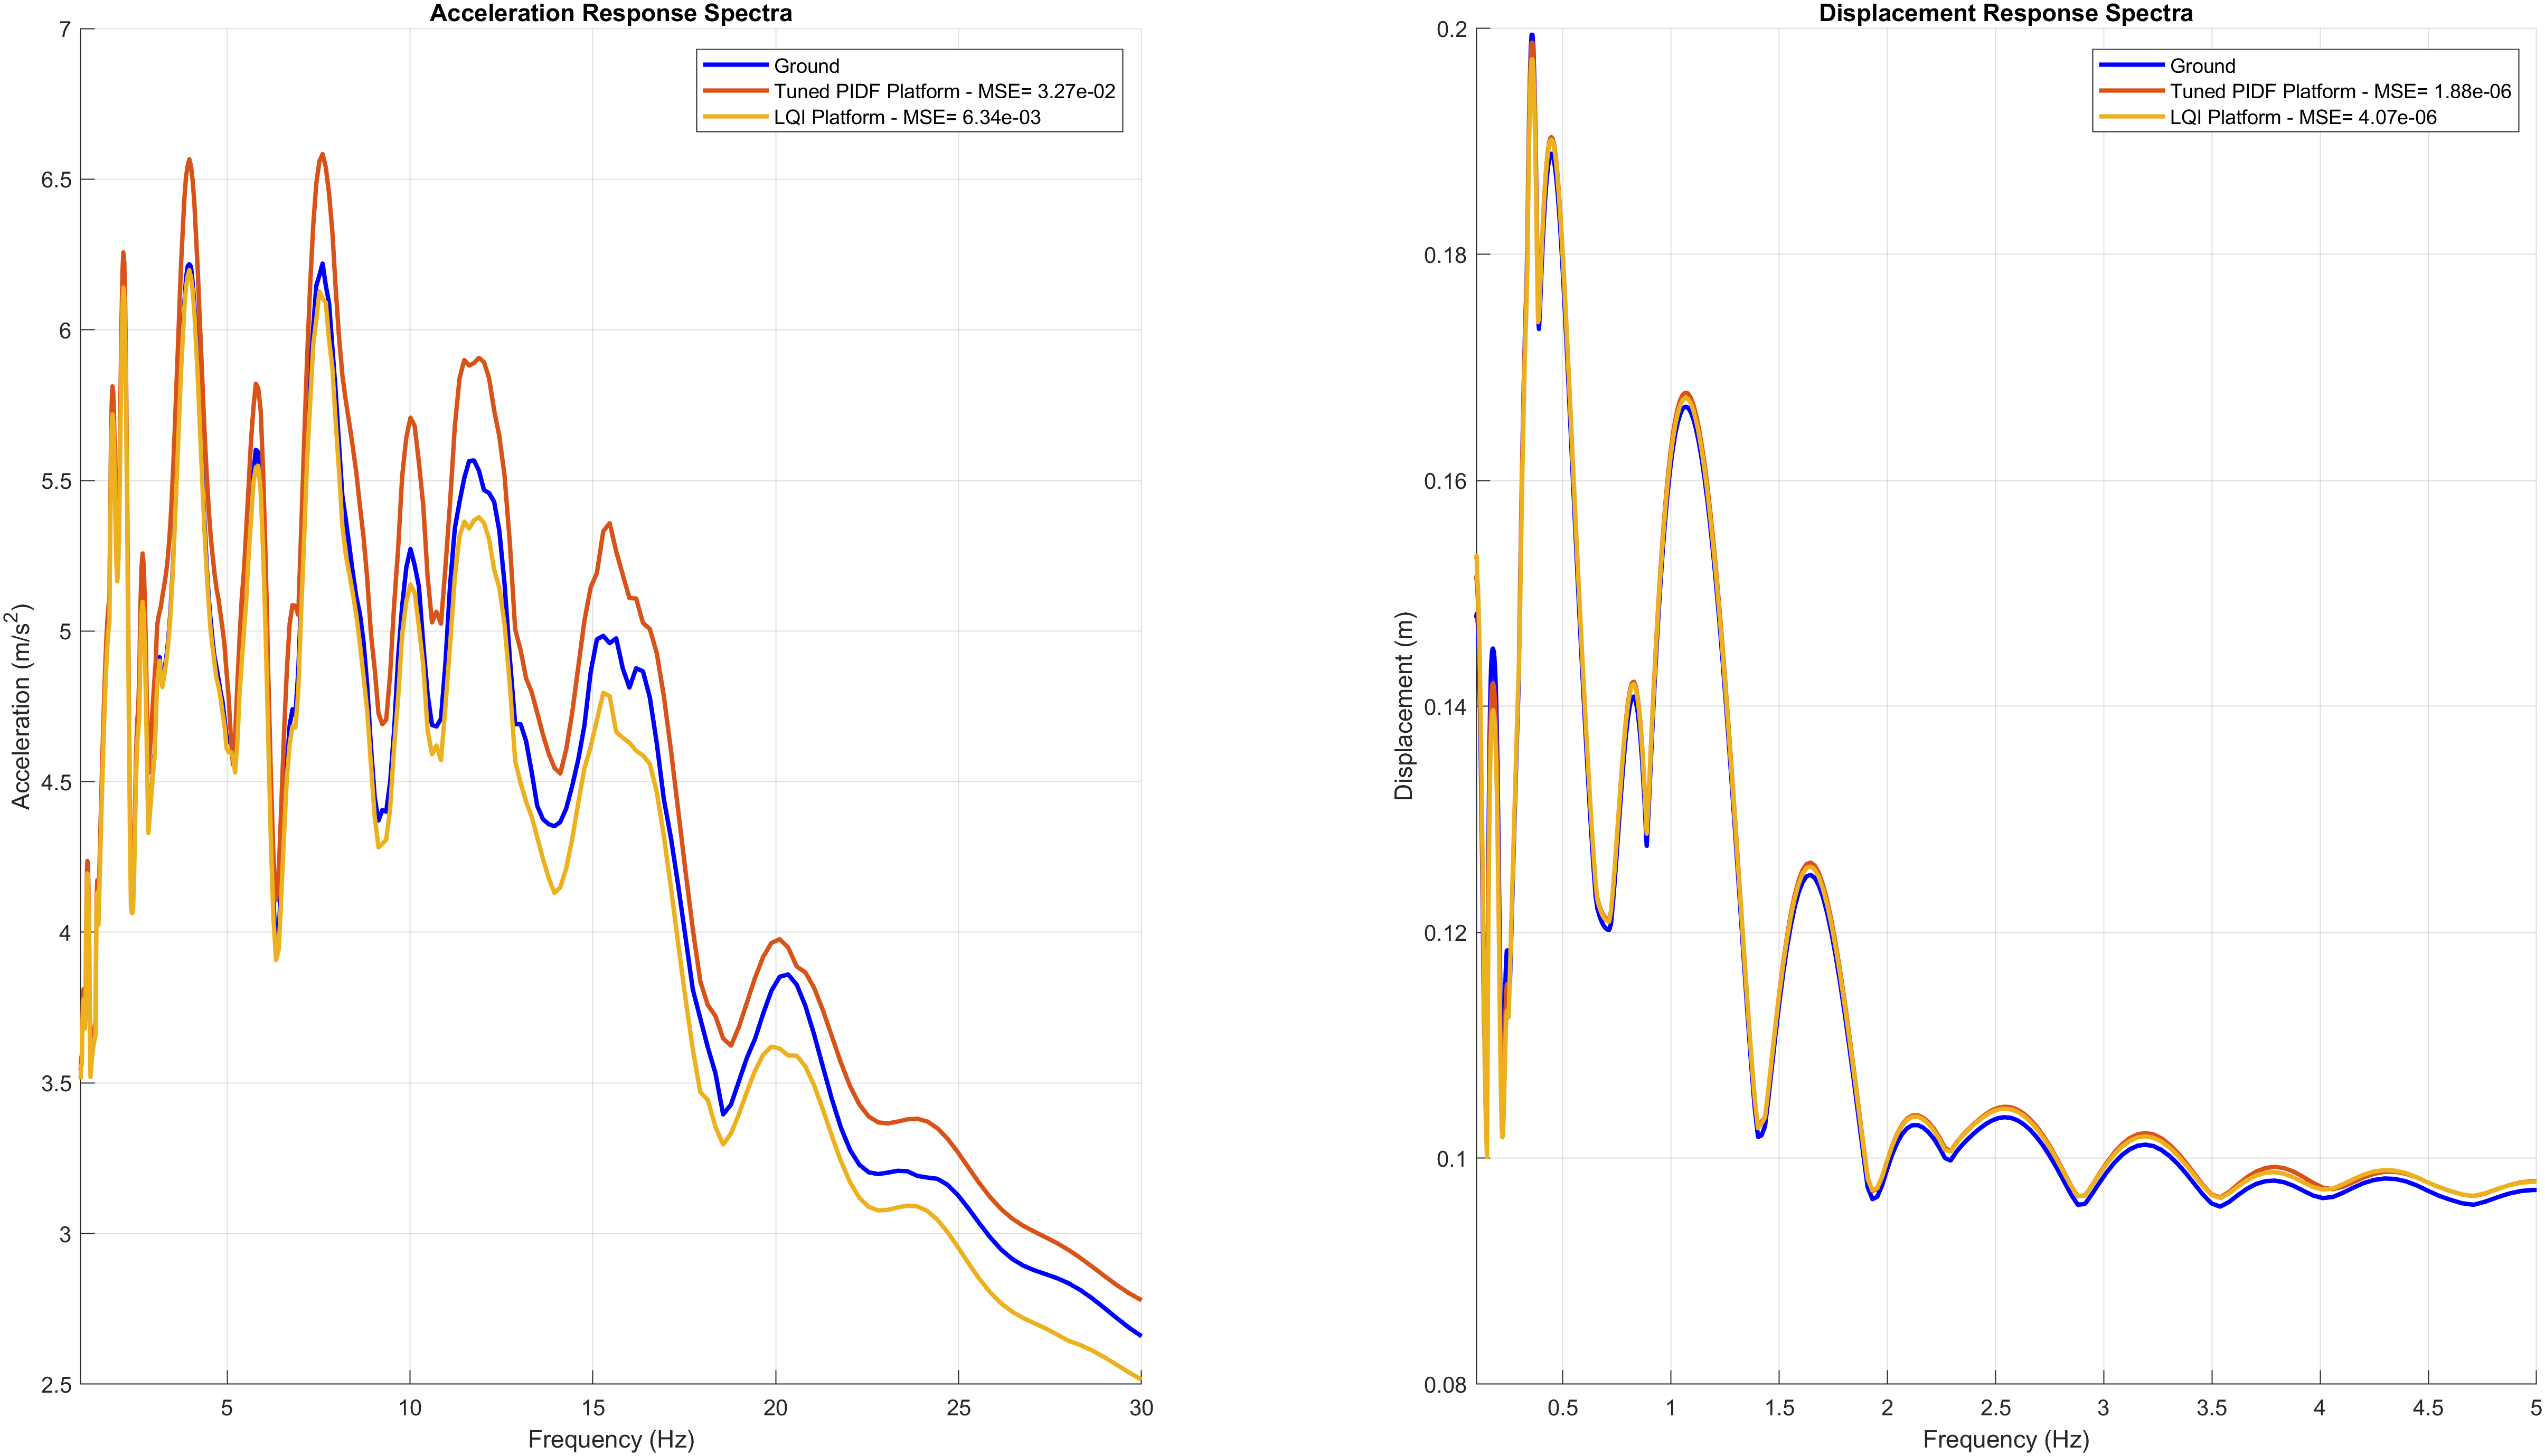
\includegraphics[width=\linewidth]{LQI/Sim_Res_Qe9_tight/Response_Spectra.png}
    \caption{Response spectrum for fault normal. The response spectrum was obtained by sampling 500 frequencies logarithmically spaced between 0.1 and 30 Hz}%, and then applying a moving average filter with a window size of 25 points.}
    \label{fig_resp_spectrum_LQI_Qe9}
\end{figure}


\begin{figure}[H]
\begin{minipage}{0.49\textwidth}
    \centering
    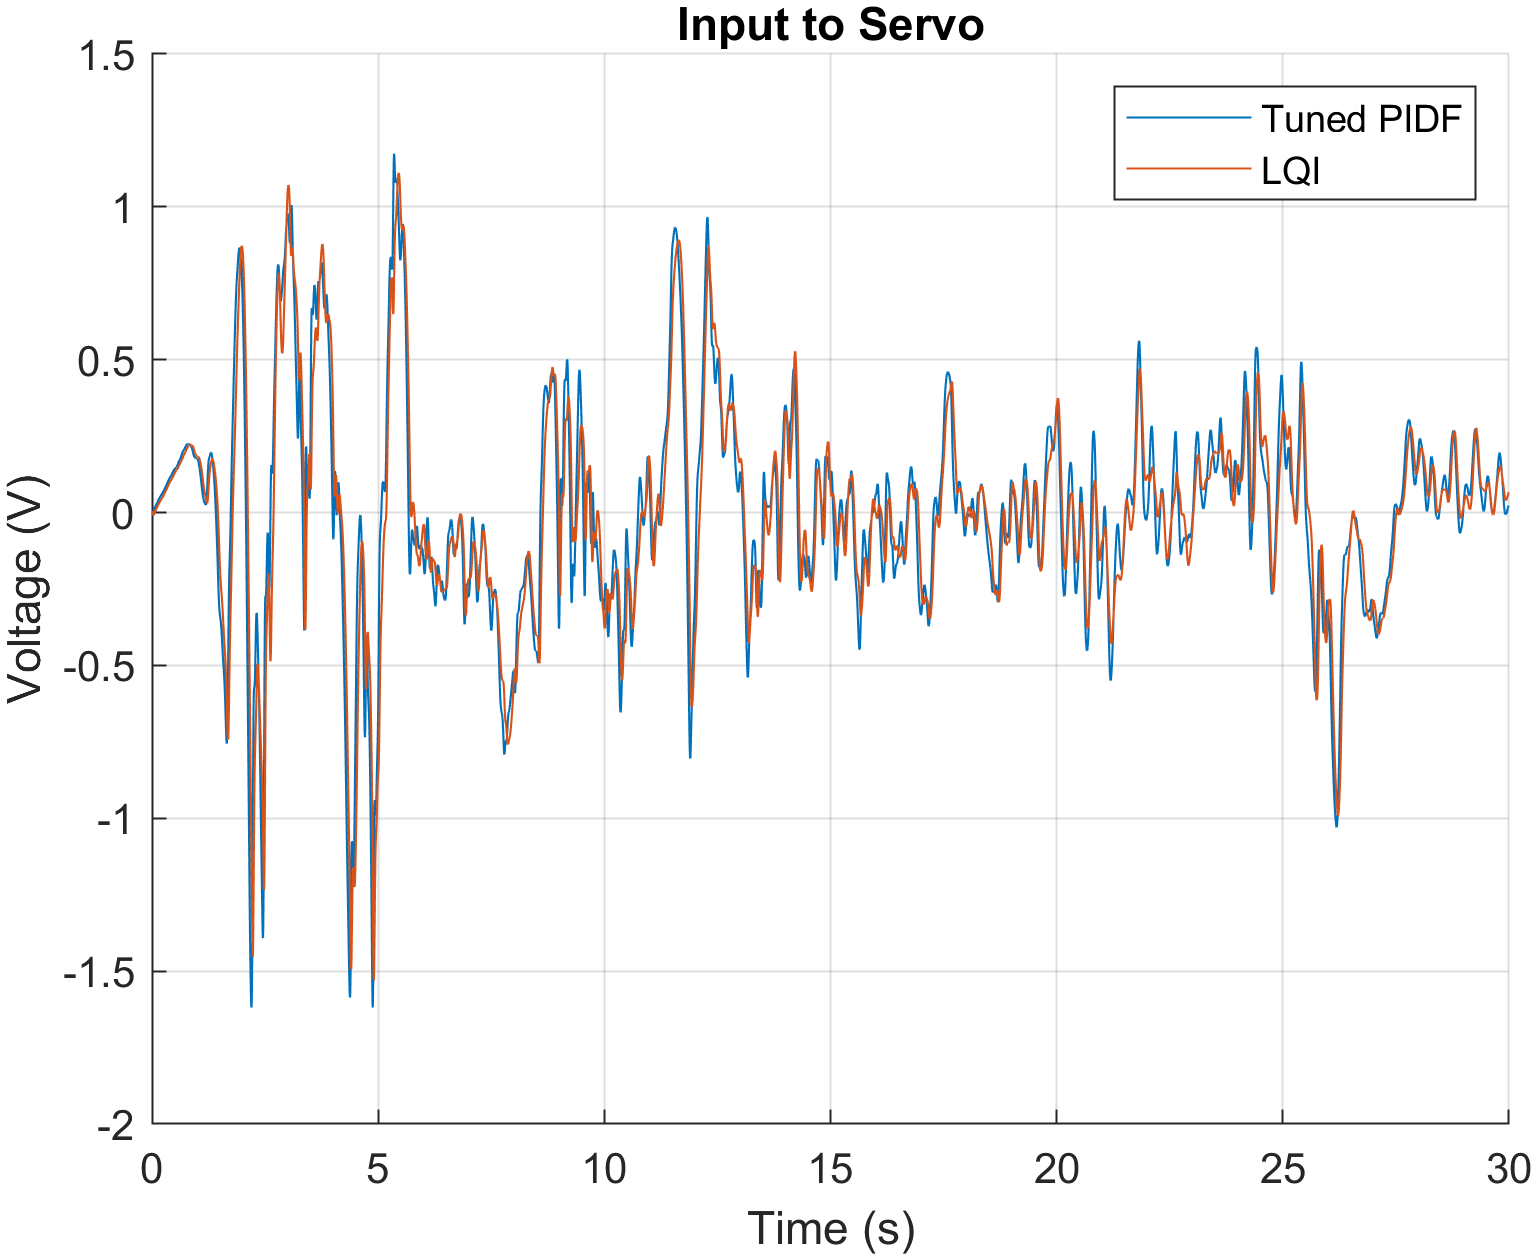
\includegraphics[width=\linewidth]{LQI/Sim_Res_Qe9_tight/Input_to_Servo.png}
    \caption{Input to servo}
    \label{fig_Input_to_Servo_LQI_Qe9}
\end{minipage}
\hfill
\begin{minipage}{0.49\textwidth}
    \centering
    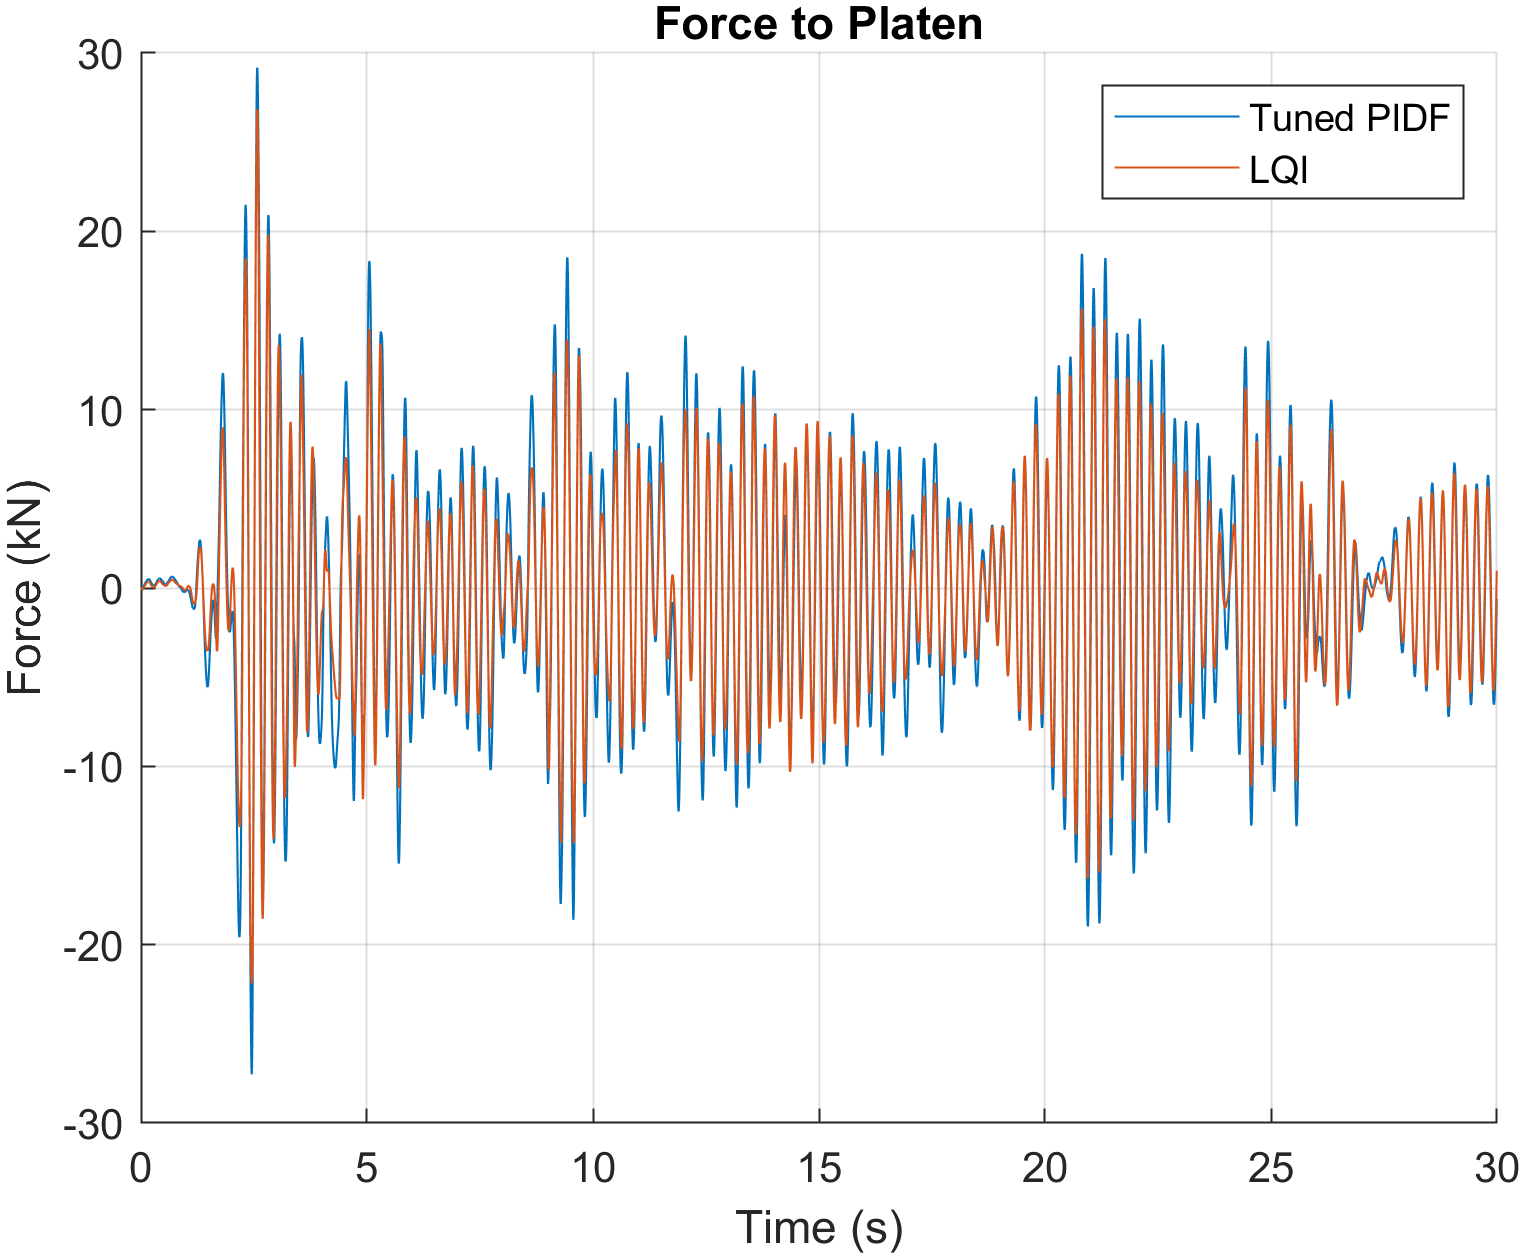
\includegraphics[width=\linewidth]{LQI/Sim_Res_Qe9_tight/Force_to_Platen.png}
    \caption{Force to Platen}
    \label{fig_Force_LQI_Qe9} 
\end{minipage}
\end{figure}
   
\begin{figure}[H]
\begin{minipage}{0.49\textwidth}
    \centering
    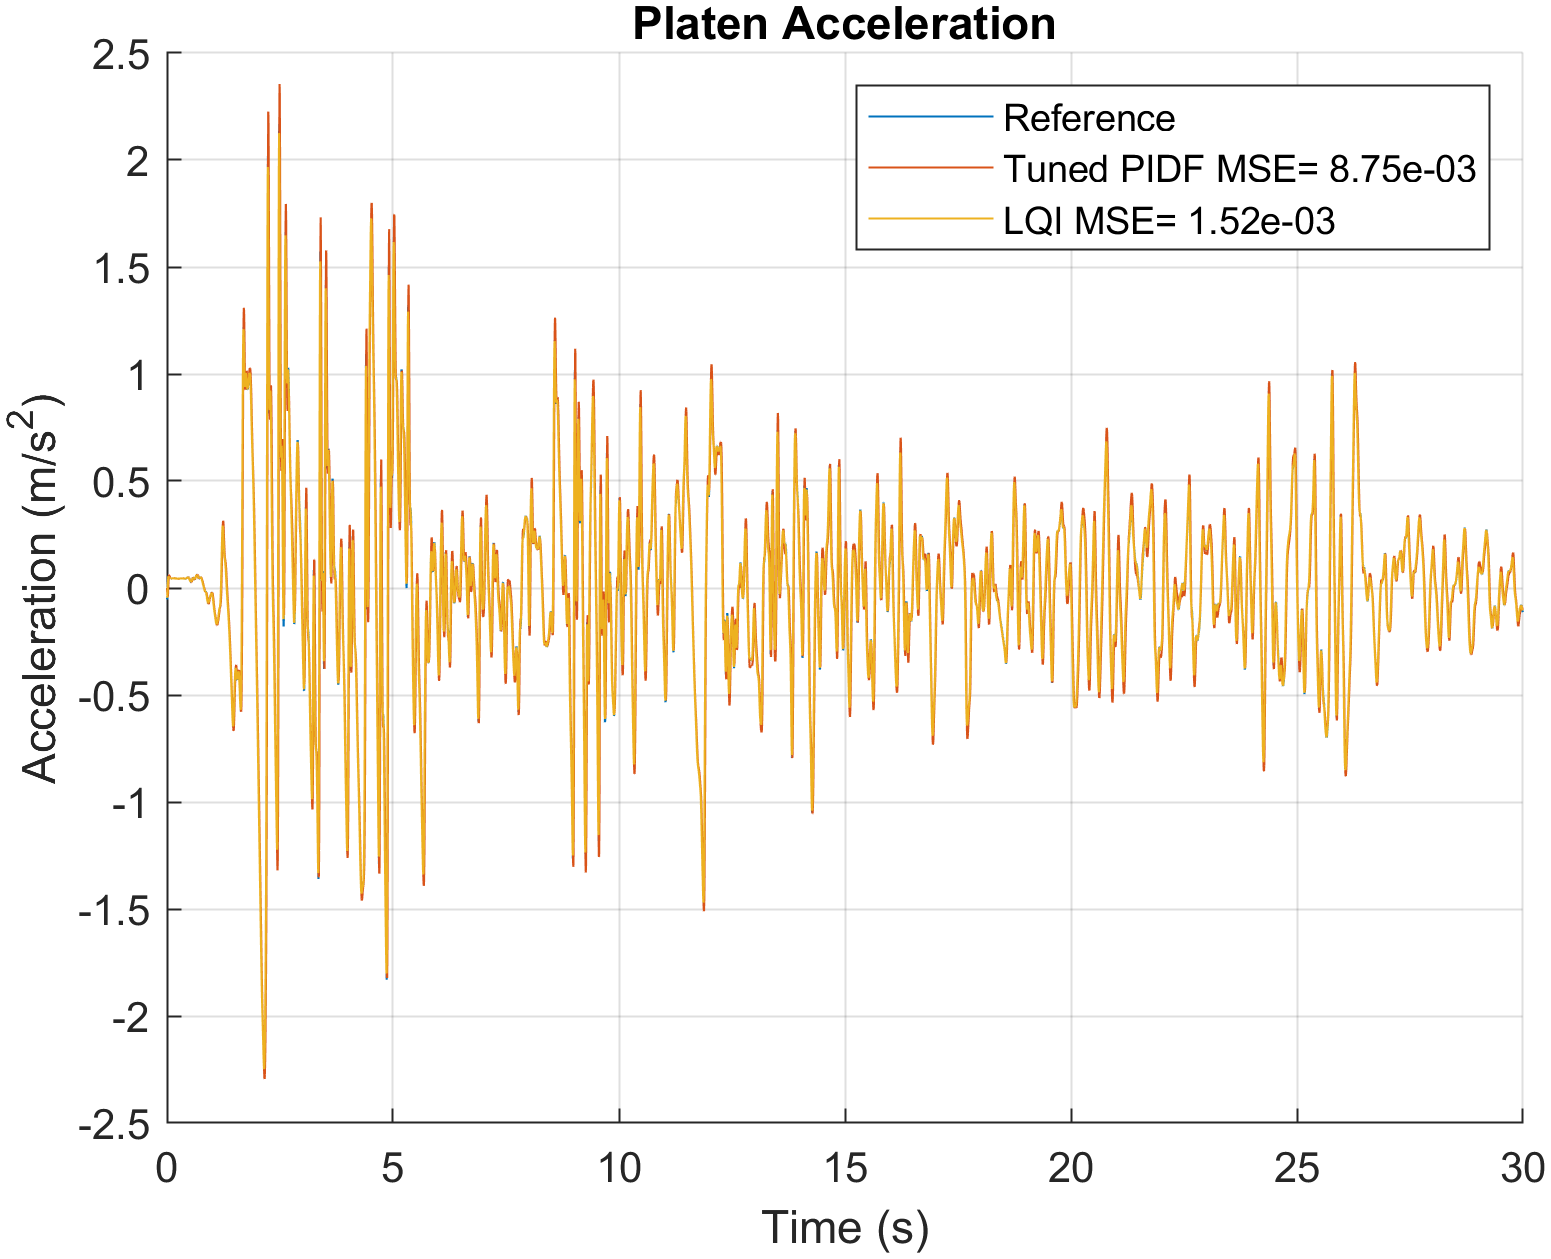
\includegraphics[width=\linewidth]{LQI/Sim_Res_Qe9_tight/Platen_Acceleration.png}
    \caption{Accelerations}
    \label{fig_Platen_Acceleration_LQI_Qe9}
\end{minipage}
\hfill
\begin{minipage}{0.49\textwidth}
    \centering
    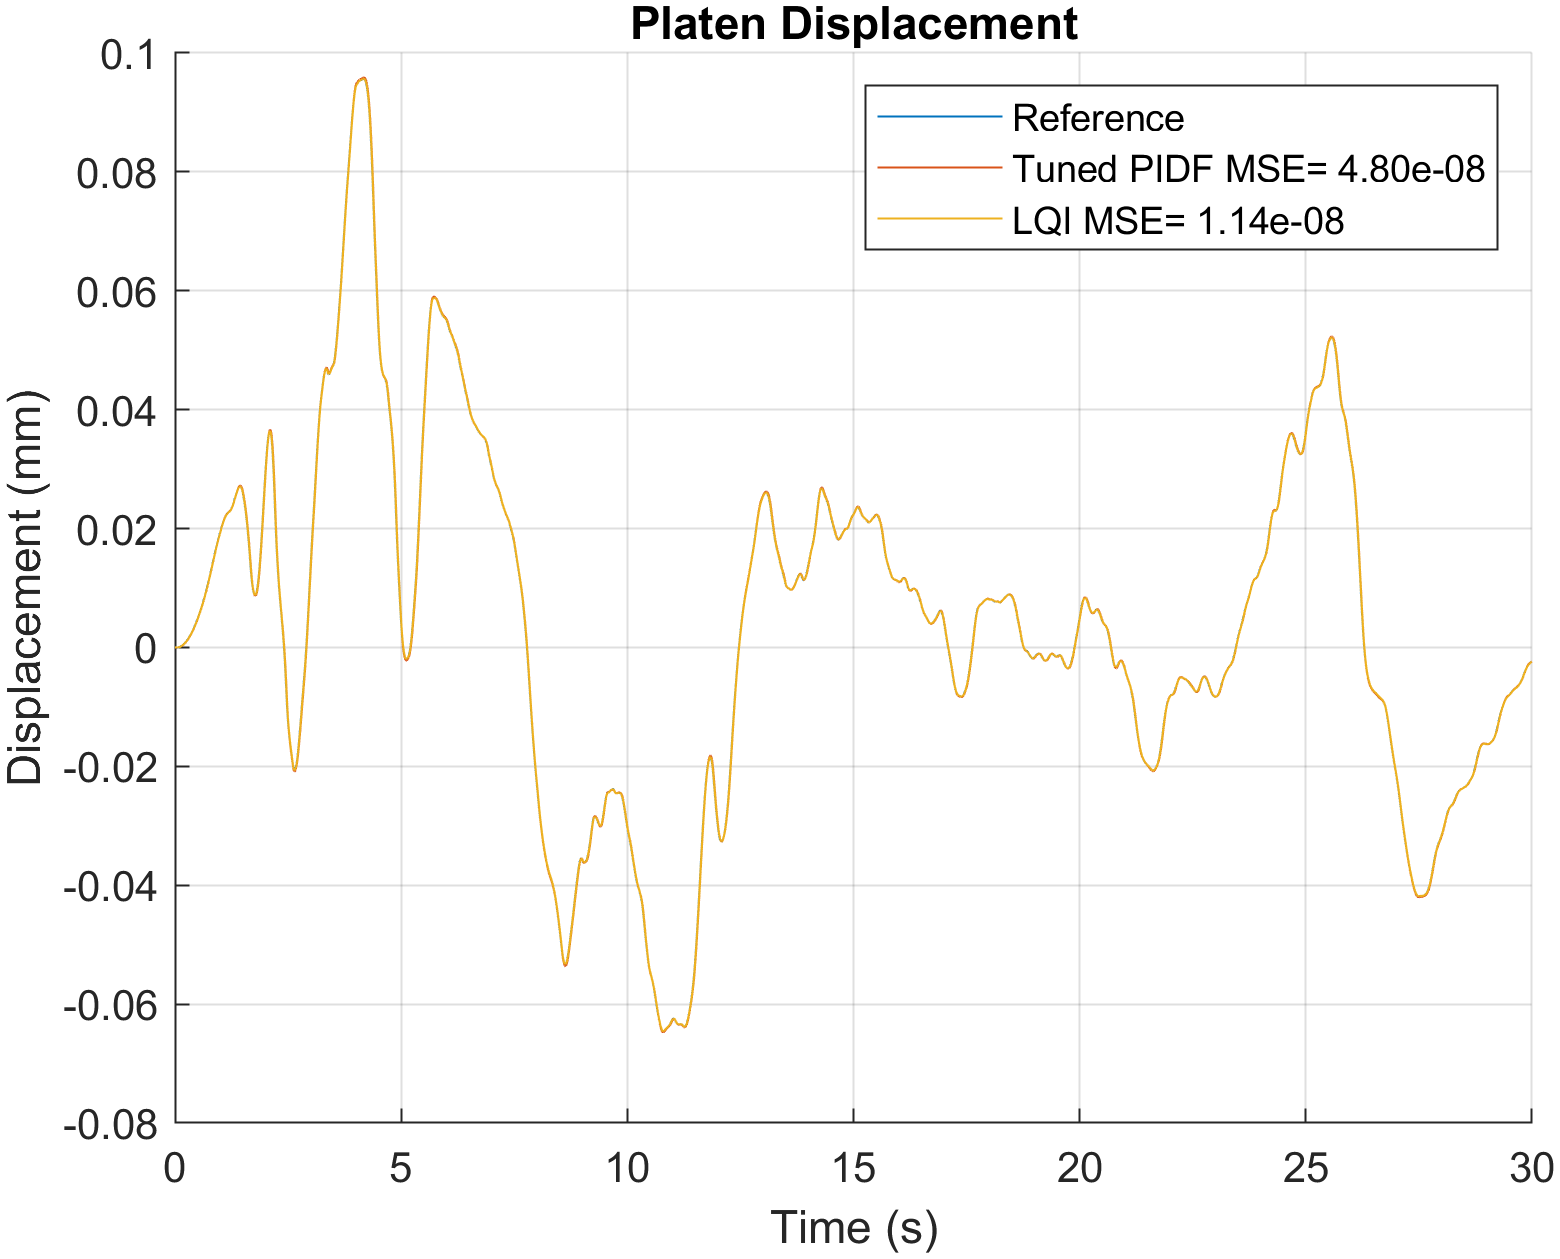
\includegraphics[width=\linewidth]{LQI/Sim_Res_Qe9_tight/Platen_Displacement.png}
    \caption{Displacements}
    \label{fig_Platen_Displacement_LQI_Qe9}
\end{minipage}
\end{figure}

\begin{figure}[H]
\begin{minipage}{0.49\textwidth}
    \centering
    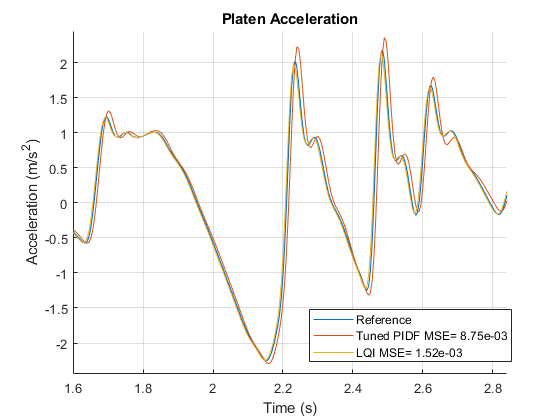
\includegraphics[width=\linewidth]{LQI/Sim_Res_Qe9_tight/Platen_Acceleration_zoom.png}
    \caption{Accelerations - Detailed view of the signals covering the period between 1.6 and 2.8 seconds}
    \label{fig_Platen_Acceleration_zoom_LQI_Qe9}
\end{minipage}
\hfill
\begin{minipage}{0.49\textwidth}
    \centering
    \includegraphics[width=\linewidth]{LQI/Sim_Res_Qe9_tight/Platen_Displacement_zoom.png}
    \caption{Displacements - Detailed view of the signals covering the period between 14.2 and 15.7 seconds}
    \label{fig_Platen_Displacement_zoom_LQI_Qe9}
\end{minipage}
\end{figure}

\begin{figure}[H]
\begin{minipage}{0.49\textwidth}
    \centering
    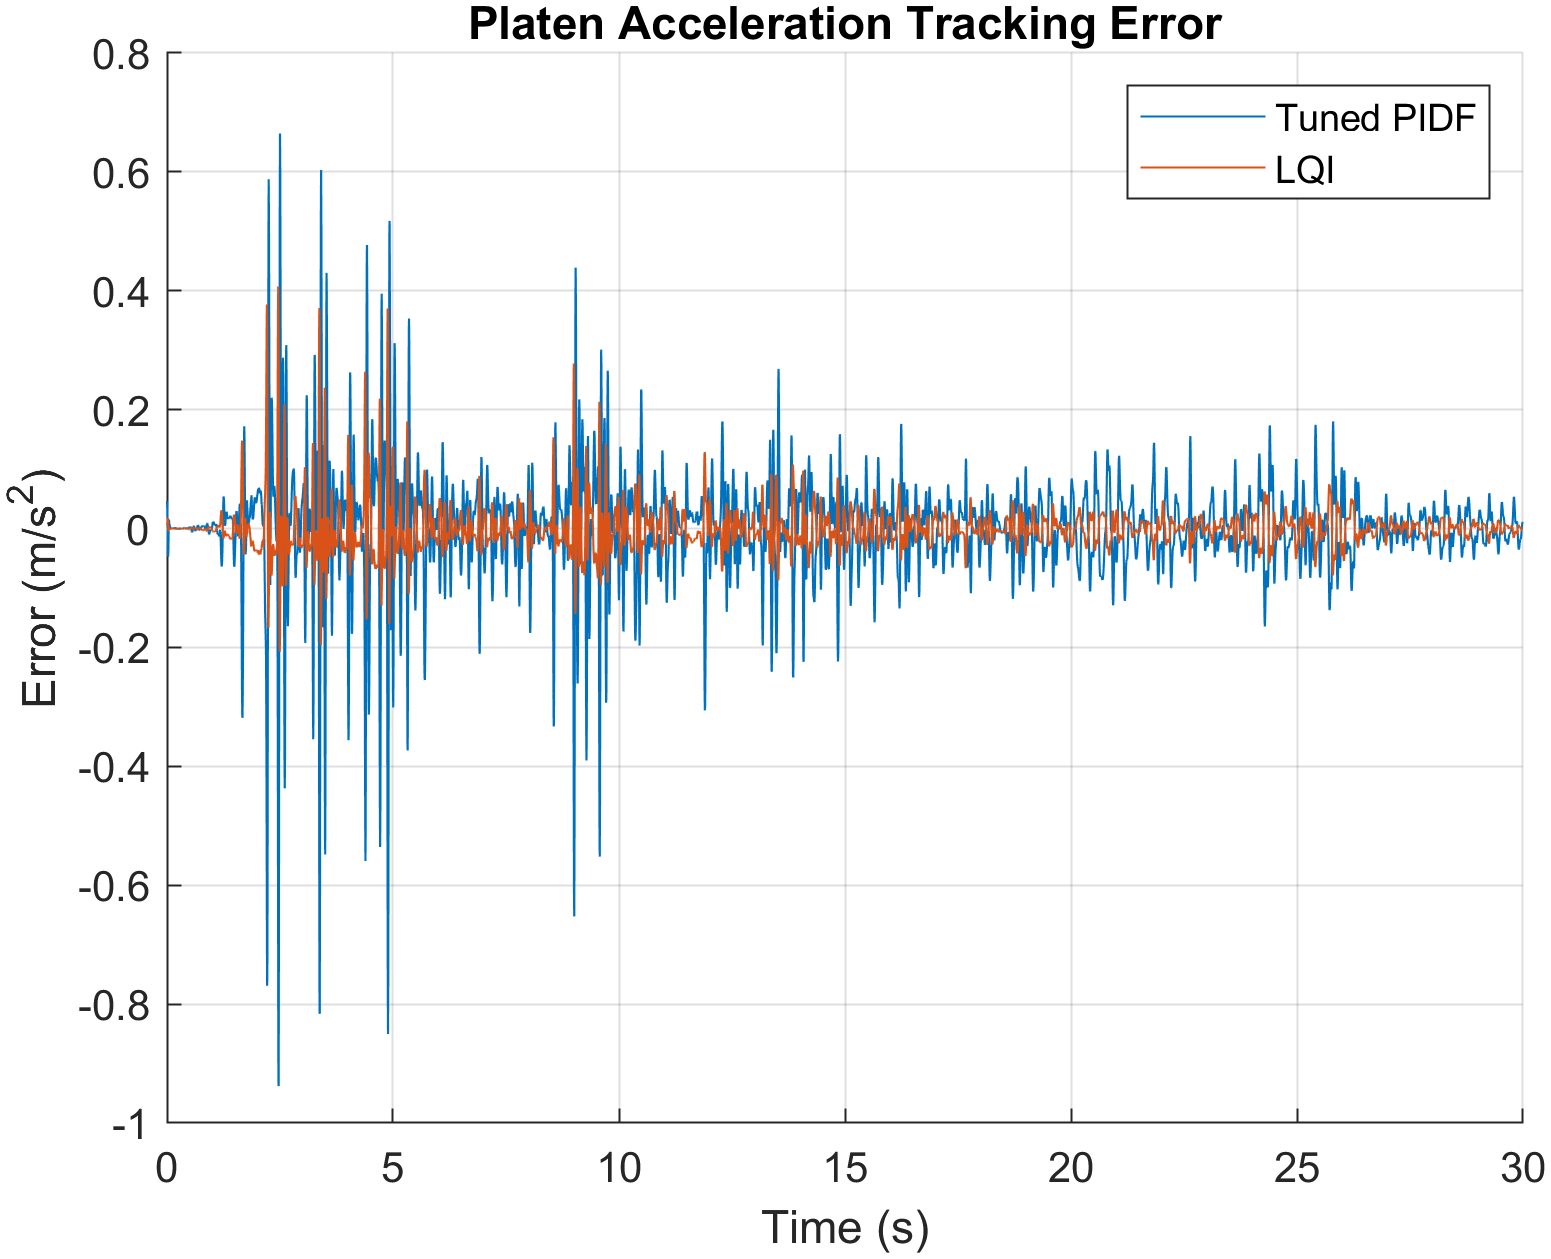
\includegraphics[width=\linewidth]{LQI/Sim_Res_Qe9_tight/Platen_Acceleration_Tracking_Error.png}
    \caption{Acceleration tracking error}
    \label{fig_Platen_Acceleration_Tracking_Error_LQI_Qe9}
\end{minipage}
\hfill
\begin{minipage}{0.49\textwidth}
    \centering
    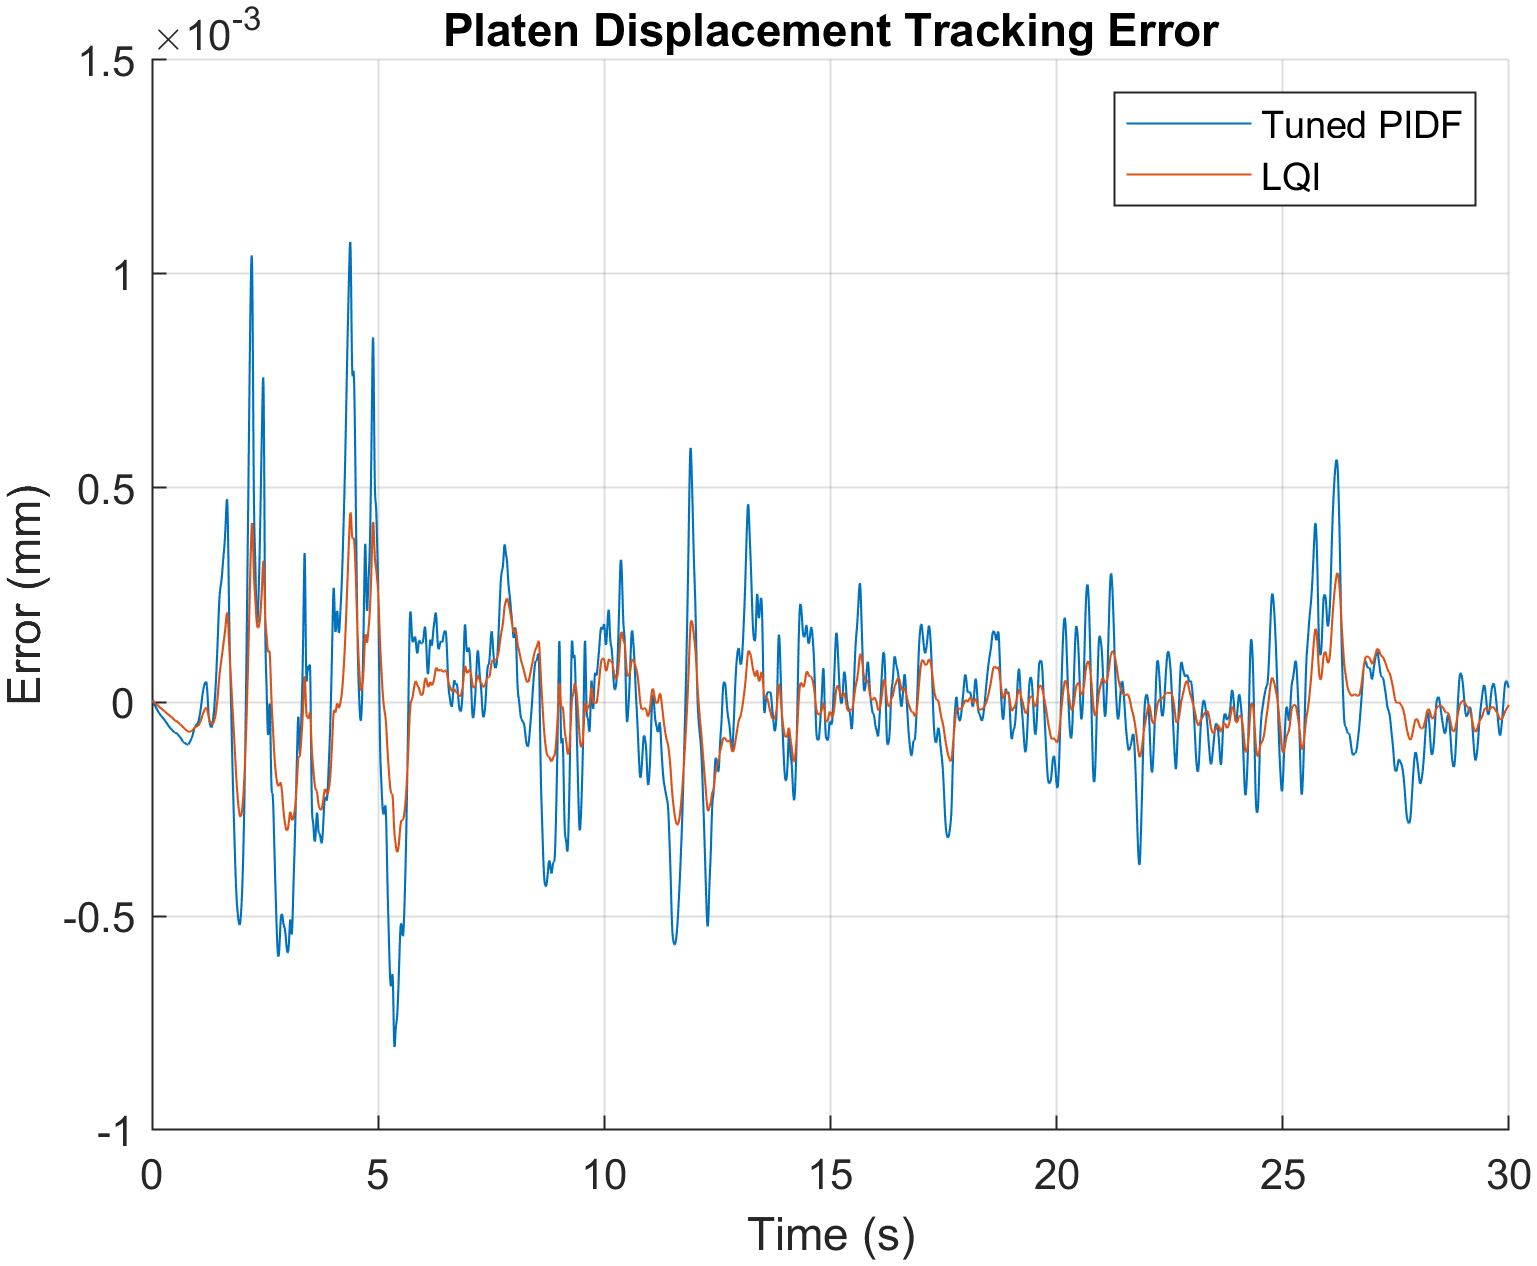
\includegraphics[width=\linewidth]{LQI/Sim_Res_Qe9_tight/Platen_Displacement_Tracking_Error.png}
    \caption{Displacement tracking error}
    \label{fig_Platen_Displacement_Tracking_Error_LQI_Qe9}
\end{minipage}
\end{figure}

\subsubsection{LQG Servo Controller}\label{LQG Servo Controller}

\begin{figure}[H]
\begin{minipage}{0.49\textwidth}
A controller using a Kalman filter (\emph{kest} in figure \ref{fig_LQG_loop}) to reconstruct the states was also implemented, with process and sensor noise covariance matrices, $Q_n$ and $R_n$, set as identity matrices.

The Kalman estimator and the optimal state feedback control law which minimizes the cost function (equation \ref{eq_LQI_cost_function}) was computed using MATLAB \emph{lqgtrack} function.
\end{minipage}
\hfill
\begin{minipage}{0.49\textwidth}
    \centering
    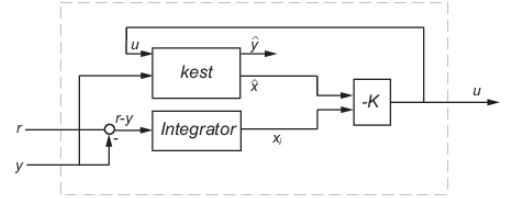
\includegraphics[width=\linewidth]{LQG/LQG_loop.png}
    \caption{LQG loop}
    \label{fig_LQG_loop}
    \end{minipage}
\end{figure}

\begin{figure}[H]
    \centering
    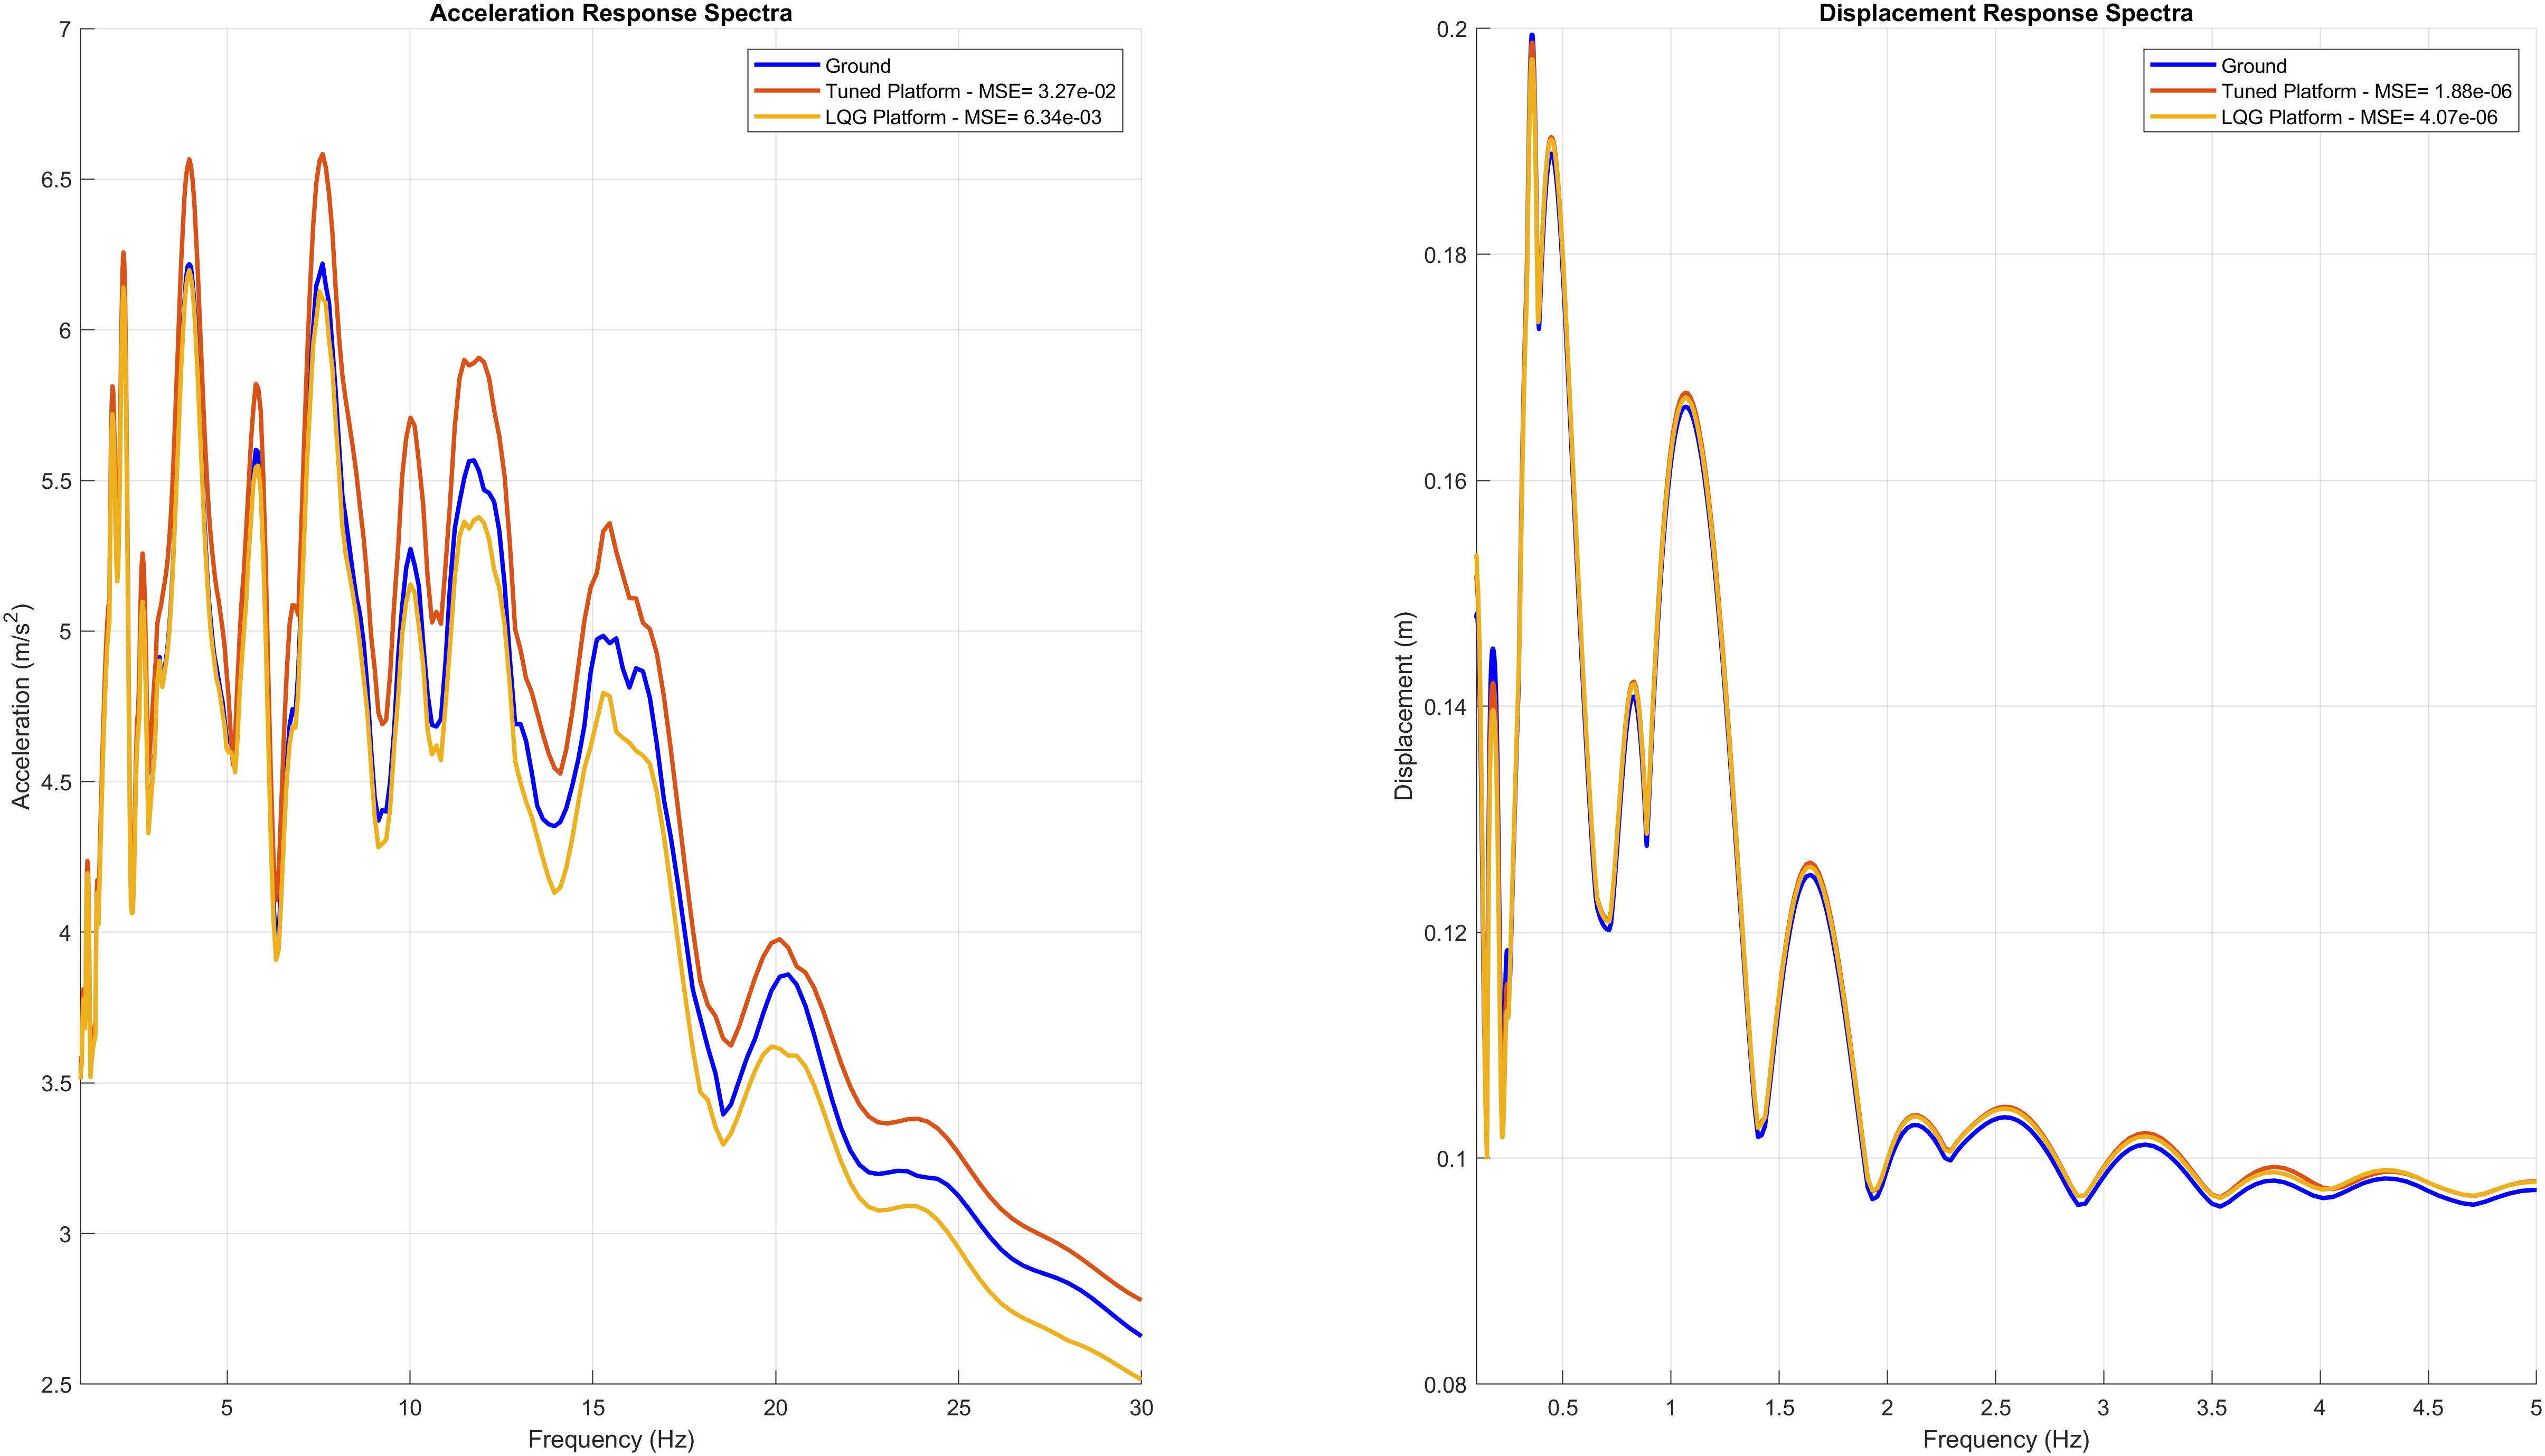
\includegraphics[width=\linewidth]{LQG/Sim_Res_Qe9_tight/Response_Spectra.png}
    \caption{Response spectrum for fault normal. The response spectrum was obtained by sampling 500 frequencies logarithmically spaced between 0.1 and 30 Hz}%, and then applying a moving average filter with a window size of 25 points.}
    \label{fig_resp_spectrum_LQG_Qe9}
\end{figure}


\begin{figure}[H]
\begin{minipage}{0.49\textwidth}
    \centering
    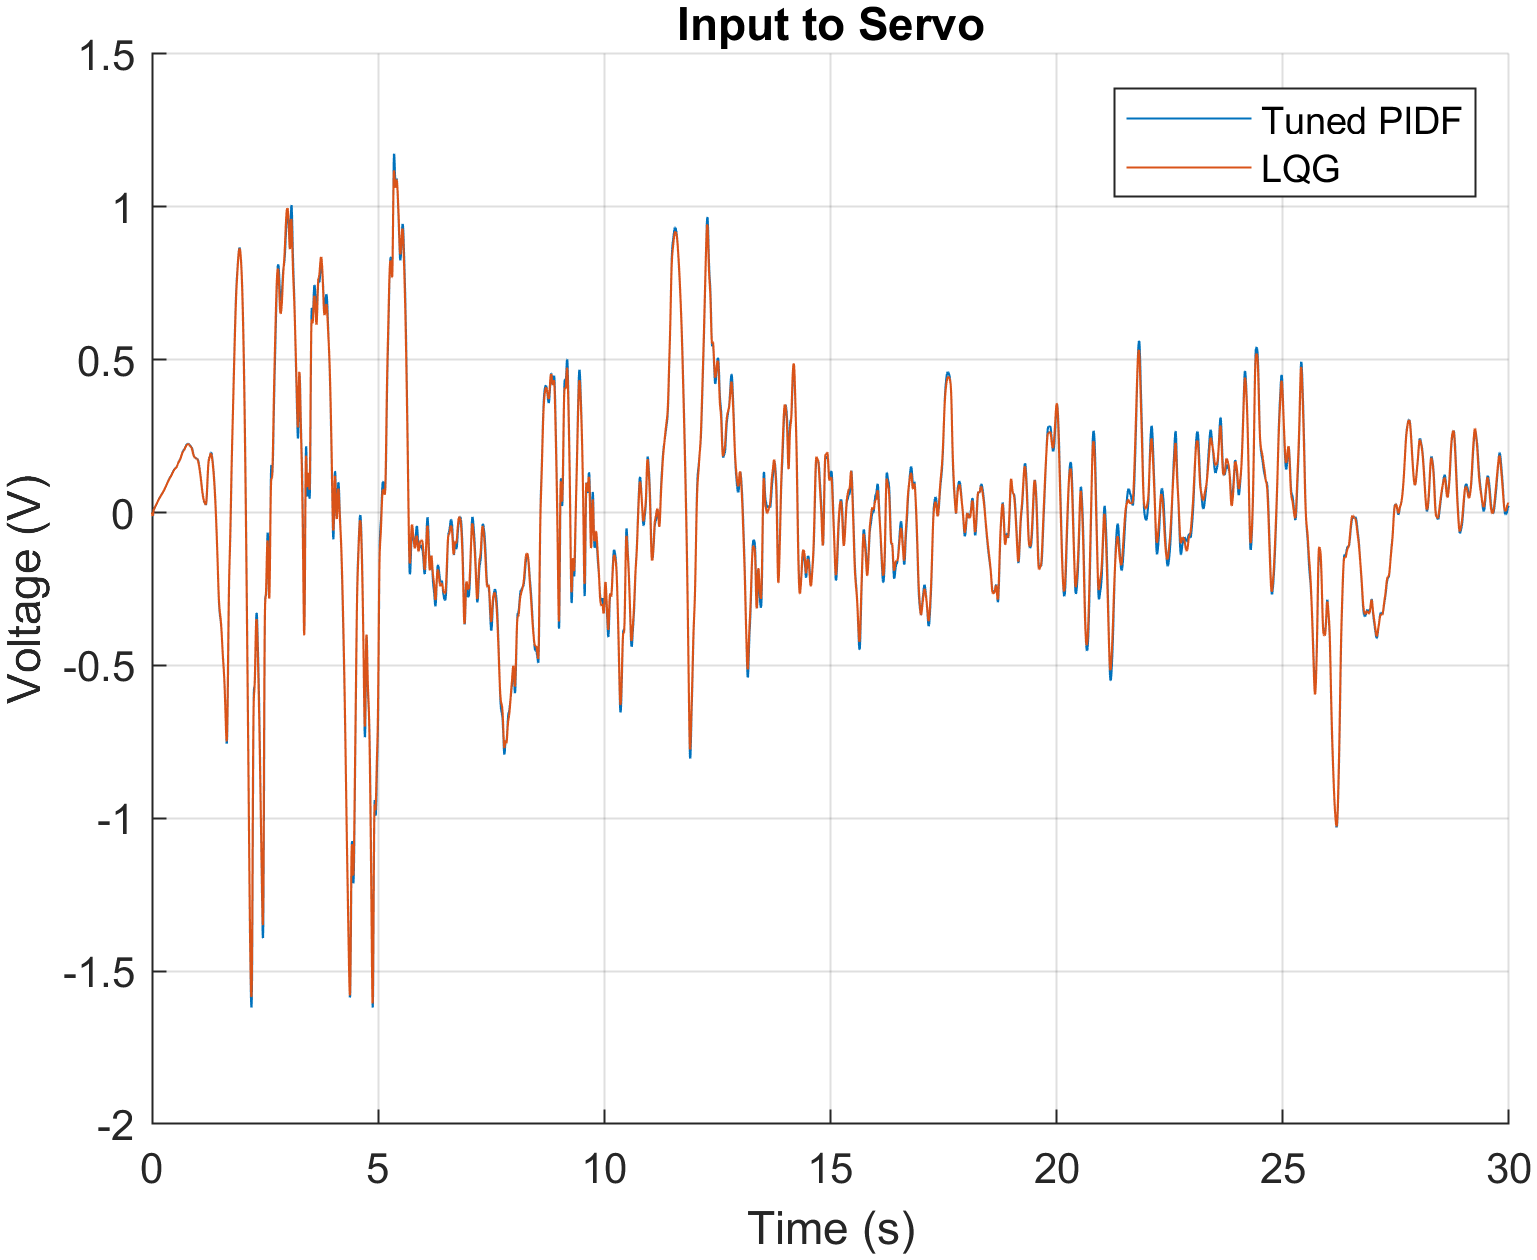
\includegraphics[width=\linewidth]{LQG/Sim_Res_Qe9_tight/Input_to_Servo.png}
    \caption{Input to servo}
    \label{fig_Input_to_Servo_LQG_Qe9}
\end{minipage}
\hfill
\begin{minipage}{0.49\textwidth}
    \centering
    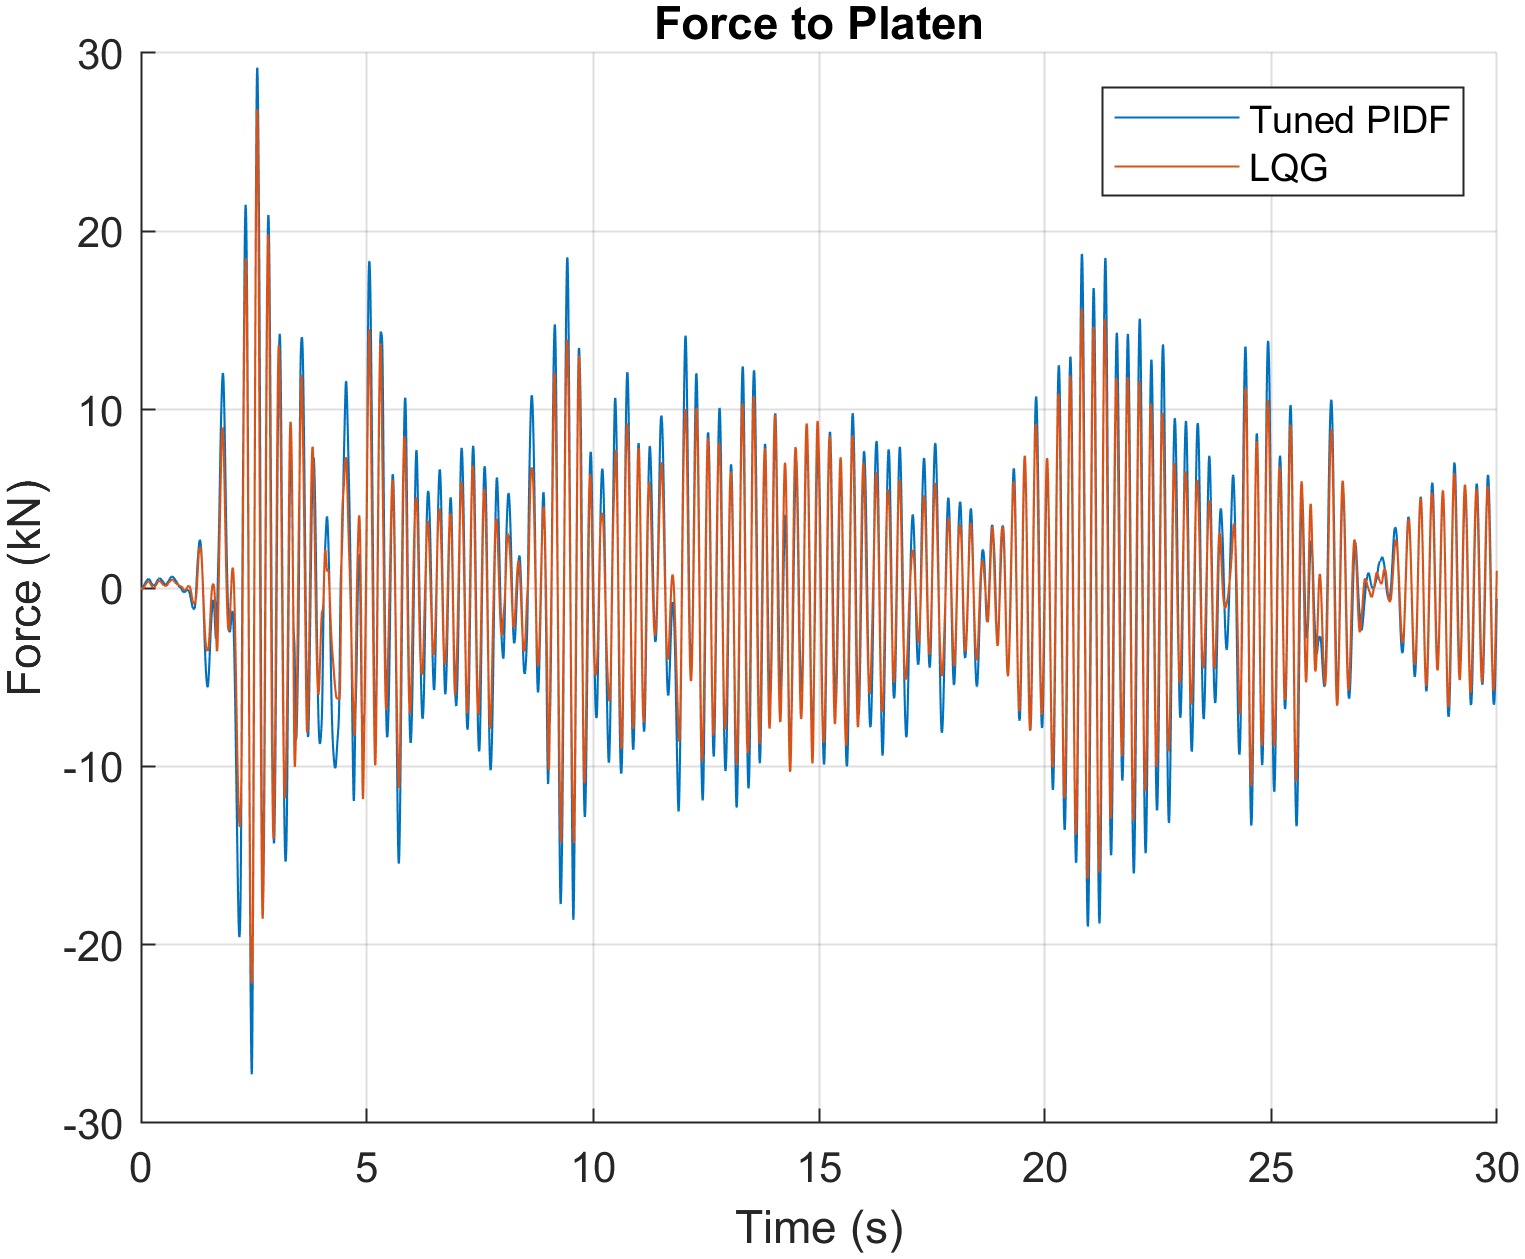
\includegraphics[width=\linewidth]{LQG/Sim_Res_Qe9_tight/Force_to_Platen.png}
    \caption{Force to Platen}
    \label{fig_Force_LQG_Qe9} 
\end{minipage}
\end{figure}
   
\begin{figure}[H]
\begin{minipage}{0.49\textwidth}
    \centering
    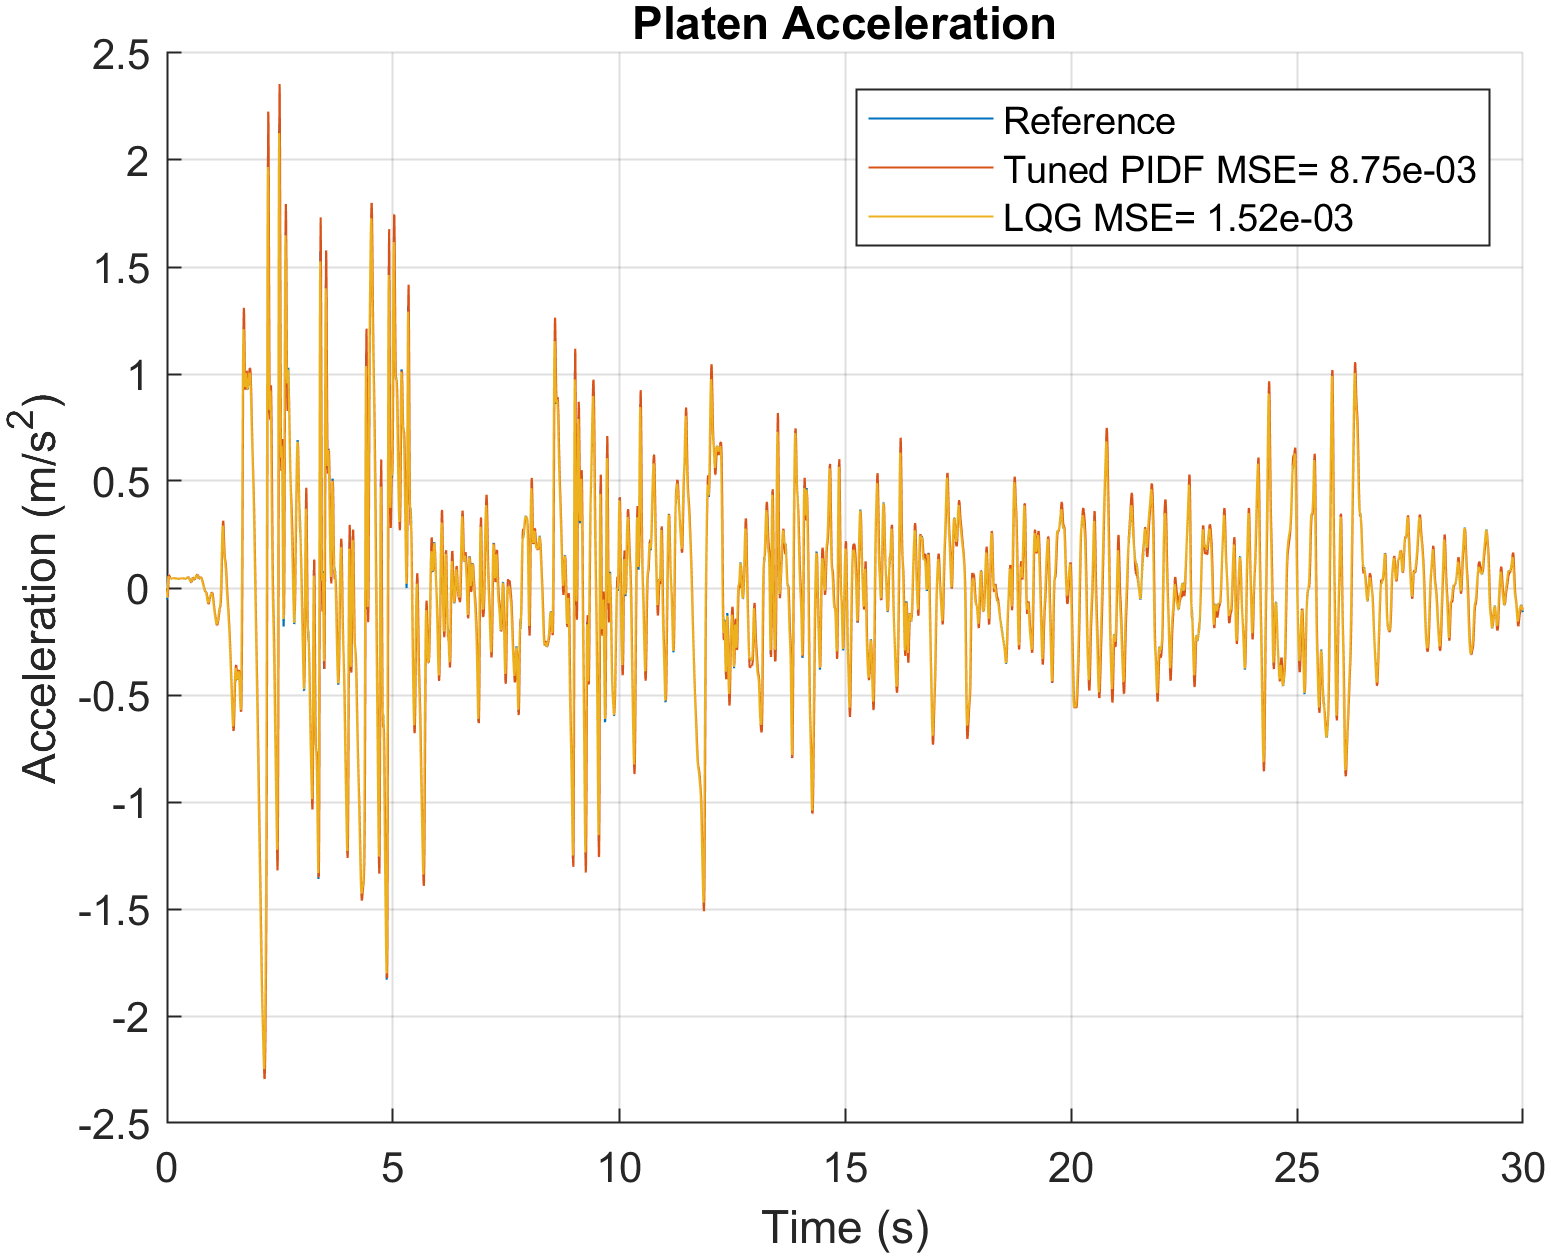
\includegraphics[width=\linewidth]{LQG/Sim_Res_Qe9_tight/Platen_Acceleration.png}
    \caption{Accelerations}
    \label{fig_Platen_Acceleration_LQG_Qe9}
\end{minipage}
\hfill
\begin{minipage}{0.49\textwidth}
    \centering
    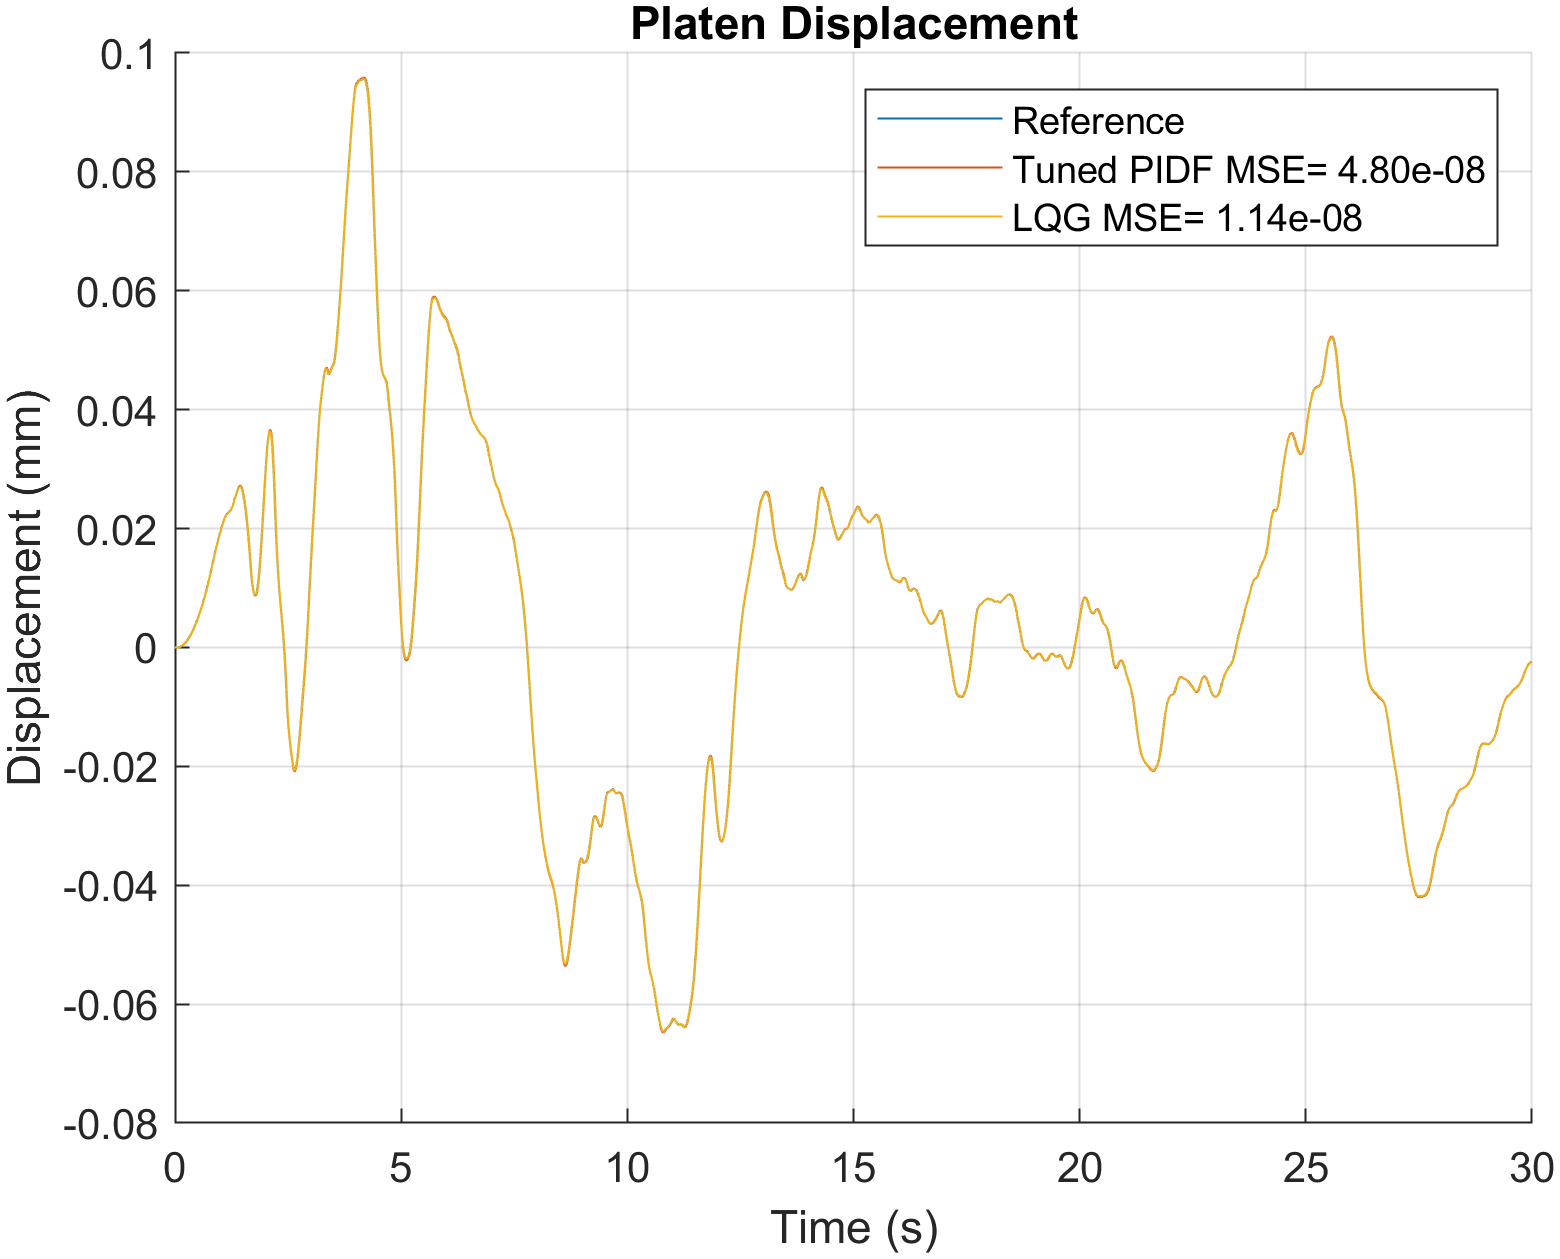
\includegraphics[width=\linewidth]{LQG/Sim_Res_Qe9_tight/Platen_Displacement.png}
    \caption{Displacements}
    \label{fig_Platen_Displacement_LQG_Qe9}
\end{minipage}
\end{figure}

% \begin{figure}[H]
% \begin{minipage}{0.49\textwidth}
%     \centering
%     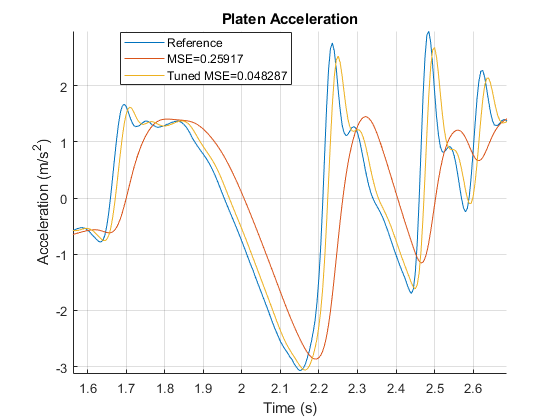
\includegraphics[width=\linewidth]{LQG/Sim_Res_Qe9_tight/Platen_Acceleration_zoom.png}
%     \caption{Accelerations - Detailed view of the signals covering the period between 1.6 and 2.8 seconds}
%     \label{fig_Platen_Acceleration_zoom_LQG_Qe9}
% \end{minipage}
% \hfill
% \begin{minipage}{0.49\textwidth}
%     \centering
%     \includegraphics[width=\linewidth]{LQG/Sim_Res_Qe9_tight/Platen_Displacement_zoom.png}
%     \caption{Displacements - Detailed view of the signals covering the period between 14.2 and 15.7 seconds}
%     \label{fig_Platen_Displacement_zoom_LQG_Qe9}
% \end{minipage}
% \end{figure}

\begin{figure}[H]
\begin{minipage}{0.49\textwidth}
    \centering
    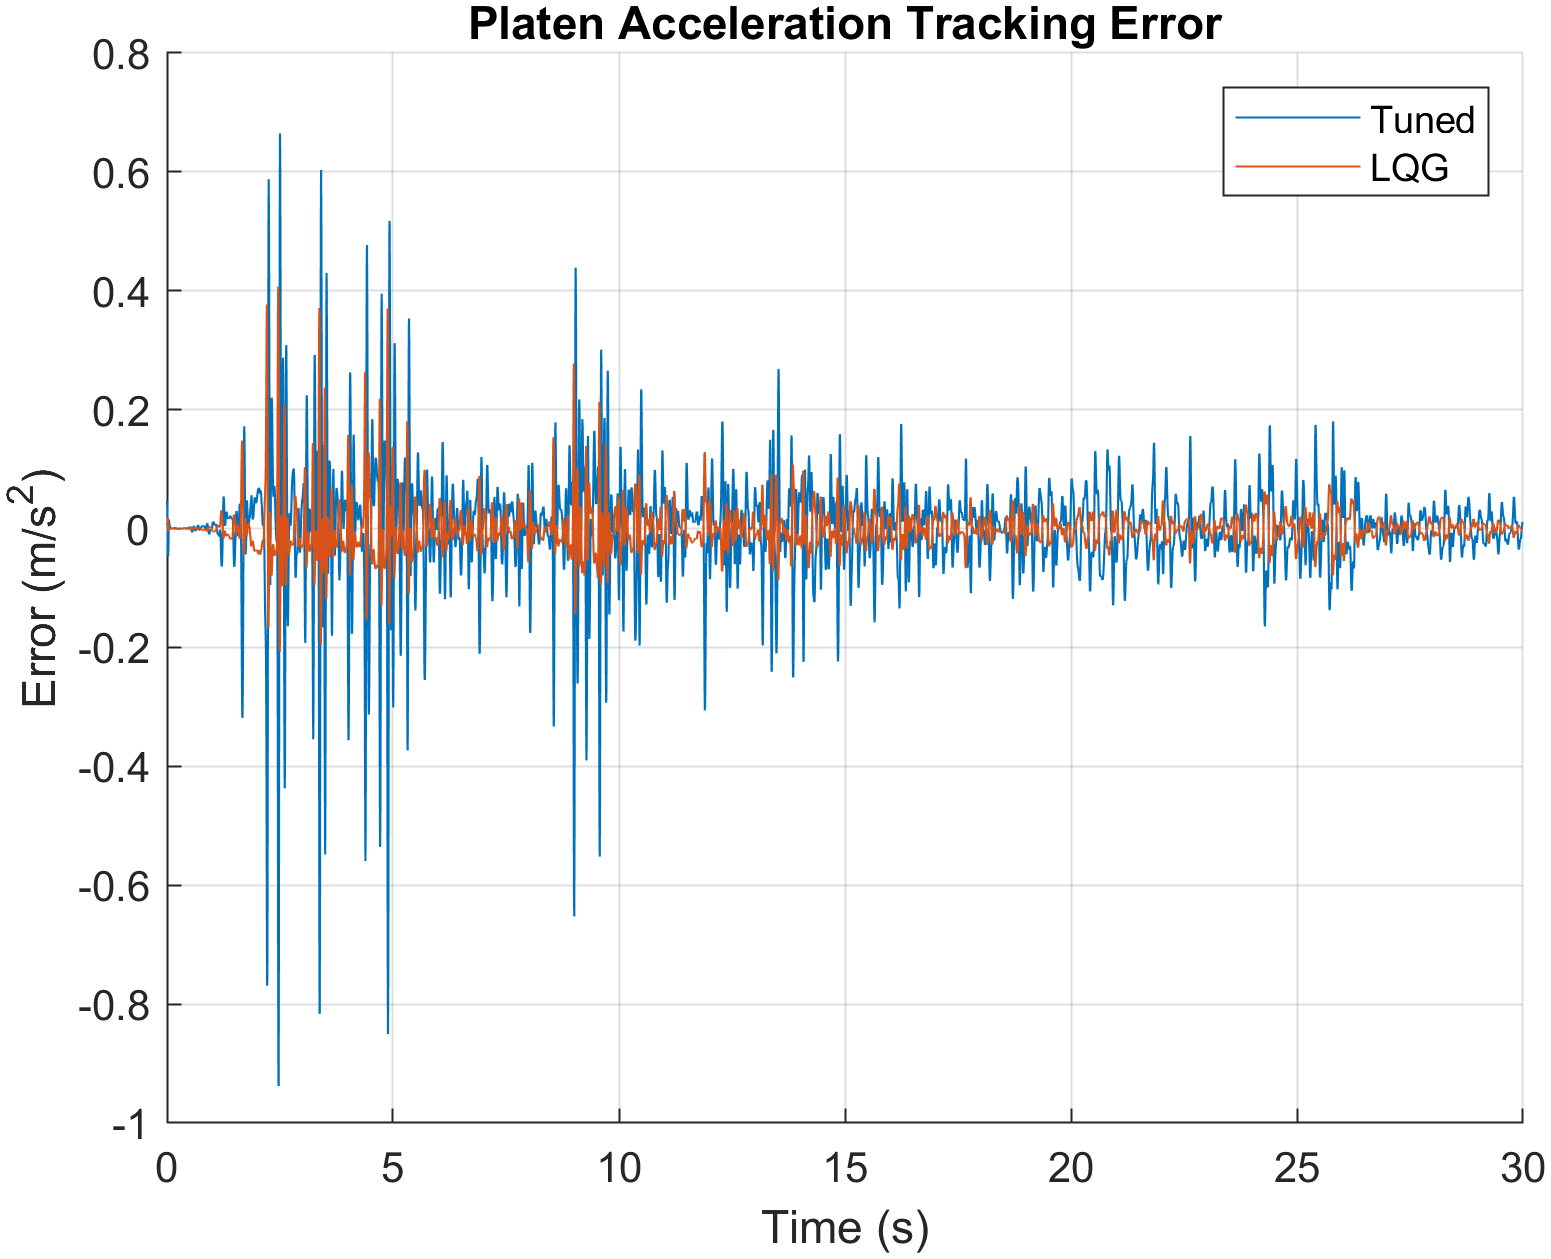
\includegraphics[width=\linewidth]{LQG/Sim_Res_Qe9_tight/Platen_Acceleration_Tracking_Error.png}
    \caption{Acceleration tracking error}
    \label{fig_Platen_Acceleration_Tracking_Error_LQG_Qe9}
\end{minipage}
\hfill
\begin{minipage}{0.49\textwidth}
    \centering
    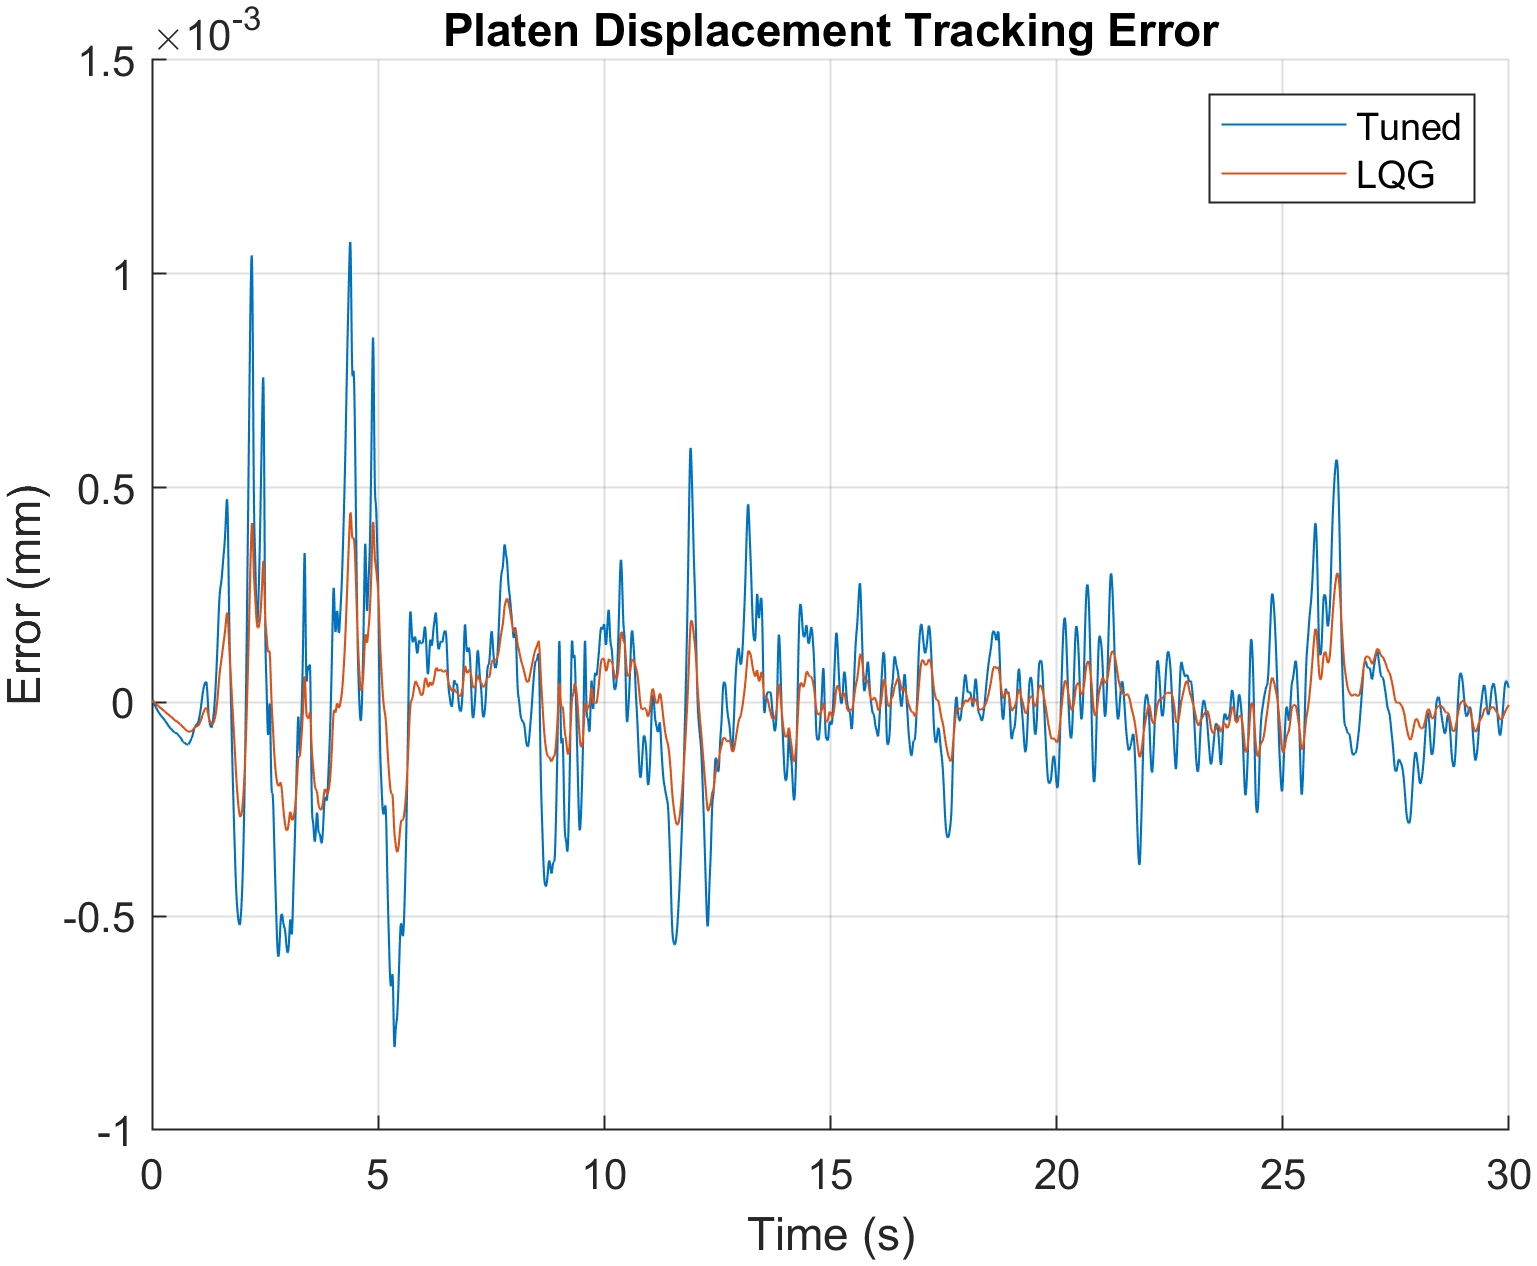
\includegraphics[width=\linewidth]{LQG/Sim_Res_Qe9_tight/Platen_Displacement_Tracking_Error.png}
    \caption{Displacement tracking error}
    \label{fig_Platen_Displacement_Tracking_Error_LQG_Qe9}
\end{minipage}
\end{figure}


\subsection{Conclusions on Simulation Results}
Using optimal control results in a much more precise replication of the ground response spectra at low frequencies, unlike the tuned PIDF which exceeds the desired response spectra in the same band. However, the trade-off for this accuracy at lower frequencies is a response spectra that falls short at higher ones. 

The optimal controller can be tuned for increasingly larger cut off frequencies without undesired amplification at low frequency, unlike the PIDF, but the results of this is practice may differ from the simulation studies preformed using the current model.

%%%%%%%% %%%%%%%% %%%%%%%%%%%%%%%%%%%%%%%%%%%%%%%%%%%%%%%%%%%%%%%%%%%%%%%%
\section{LNEC's seismic platform driver signal adaptation process}

\begin{figure}[H]
\begin{minipage}{0.4\textwidth}
    \centering
    \includegraphics[width=\linewidth]{Adapt/driver_signal_generation_loop.png}
    \caption{A simplified block diagram of driver signal modification loop}
    \label{driver_signal_generation_loop}
\end{minipage}
\hfill
\begin{minipage}{0.55\textwidth}
    \subsection{The functioning of the driver adaptation software}
As seen in the previous chapters, the use of a proportional controller for tracking the position reference signal does not produce the desired performance from the seismic table in terms of response spectrum. 

An attempt to improve the seismic table performance at LNEC comes in the form of pseudo-open loop control, whereby, before every test run, a proprietary software %developed in LabVIEW 
called \emph{Adapt}, through a set of user-defined parameters and decisions, identifies the system transfer function, and then modifies the reference signal, creating what we will now refer to as \emph{driver signal}, which is then used as the reference in the closed-loop control of the seismic table position.

In the system identification menu (figure \ref{Adapt_FRF_Parameters}) the user can apply various filters to the acquired displacement and acceleration signals, and then choose how to synthesise both into a displacement signal. This is done to reject the inaccurate readings of position sensors at high frequencies, and of acceleration sensors at low frequencies, and combine the information of both to generate a more accurate displacement signal. Then the user can choose various options for the computation of the transfer function.
\end{minipage}
\end{figure}

\begin{figure}[H]
    \centering
    \includegraphics[width=1\linewidth]{Adapt/Adapt_Project_Parameters.png}
    \caption{Adapt Project Parameters menu - In this menu the user configures which files were used for determining the system's FRF, and the reference (or target) signal.}
    \label{fig:enter-label}
\end{figure}

\begin{figure}[H]
    \centering
    \includegraphics[width=0.95\linewidth]{Adapt/Adapt_FRF_Parameters.png}
    \caption{Adapt FRF Parameters menu - The modification of the driver signal requires the identification of the frequency response function of the system. In this menu the user sets parameters which are used in the composition of a displacement signal from acceleration and displacement data acquired from a test run where 3 minutes of pink noise are used as input. The user also defines the settings for the computation of the FRF.}
    \label{Adapt_FRF_Parameters}
\end{figure}

\begin{figure}[H]
    \centering
    \includegraphics[width=0.95\linewidth]{Adapt/Adapt_INV_Panel.png}
    \caption{Adapt INV Panel menu - This menu is used to generate new driver signals, and takes as inputs the original reference (referred to as \emph{target}), the driver signal used in the test run, it's measured output at the seismic table, and user defined parameters which affect which parts of the signal are modified, and by how much they're modified.}
    \label{Adapt_INV_Panel}
\end{figure}

\subsection{Simulating the driver adaptation process}

For this section the coupled 2-dof system had both it's masses set to 2000 kg, $f_1 = 1.5 Hz$ , $\zeta_1  = 0.02$, $f_2 = 6 Hz$, $\zeta_2 = 0.05$, and the optimal controller with $Q=10^3$ (as in Figure \ref{fig_Bode_LQI_Qe3}).

\begin{figure}[H]
\begin{minipage}{0.55\textwidth}
\subsubsection{System Identification}
The first step in the driver adaptation process is identifying the system transfer function (seismic platform + model). To this end, the seismic table is run for 3 minutes with a pink noise signal as input. 

This was simulated by converting a pink noise \emph{.drv} file (a proprietary file format meant for use with LNEC proprietary software tools: \emph{LNEC SPA} and \emph{Adapt}) used in one of LNEC's seismic tests, through the use of a Python library which replicates the functioning of LNEC SPA, which allows the conversion to standard text file, and then providing this signal as input to the MATLAB model previously developed. The simulation output, seismic table position and acceleration over time, is then written to a \emph{.acq} file, again using \emph{LNEC SPA} Python library functions.

The driver and simulated acquired data files are then input to \emph{Adapt}, where the system frequency response function is determined.
\end{minipage}
\hfill
\begin{minipage}{0.4\textwidth}
     \centering
    \includegraphics[width=\linewidth]{Adapt/bode_compare.png}
    \caption{Identified frequency response function from \emph{Adapt} (using "bad" settings) versus the model from Section \ref{Modelling Seismic Table Dynamics}}
    \label{bode_compare}
\end{minipage}
\end{figure}

\subsubsection{Generating the target files (.tgt)}
The acceleration signal of each seism was integrated twice using a simple trapezoidal rule. From the obtained displacement signal, the initial and final displacement values were used to compute the average velocity, which was then used to subtract the drift from displacement signal, and have it begin and end at zero. Then the signal was scaled to fit the displacement range of seismic table (and the mathematical model).

\subsubsection{Generating the adapted driver}

The first driver (driver zero) was generated using just the target file. This driver was then converted to text format using the previously mentioned Python functions, and then input into the Matlab model. From the displacement output, the acceleration was computed using a second order central difference. This data was then written to \emph{.acq} format, and used to generate driver 1  in \emph{Adapt.exe}. The process was repeated to generate subsequent drivers.

\subsubsection{Performance Analysis}

\begin{figure}[H]
    \centering
    \includegraphics[width=1\linewidth]{Adapt/Response_Spectra.png}
    \caption{Target response spectrum and the resulting response spectrum from tuned PIDF, optimal controller, and the 3 iterations of adapted drivers resulting from FRF shown in figure \ref{bode_compare}.}
    \label{Response_Spectra_2drivers}
\end{figure}

For the seismic signal tested in this section (L'Aquila reduced scale seism), the response spectra from adapted drivers underperforms compared to the PIDF controller, and even more so when compared to the optimal controller. 

In figure \ref{Response_Spectra_better_id}, the identified FRF (figure \ref{bode_compare_better_id}) used for adapting the drivers  is closer to the model, resulting in a better adaptation of the driver signal, but it still requires 3 iterations to somewhat achieve the target response spectrum, and still doesn't perform as well as the optimal and PIDF controllers.

In figure \ref{Response_Spectra_2drivers}, the identified FRF (figure \ref{bode_compare}) used for adapting the drivers isn't as good as in the other case (figure \ref{bode_compare_better_id}), due to the settings defined by the user in \emph{Adapt}, and the resulting response spectrum after three iterations isn't very satisfactory. This shows the one of limitations of this method: It depends on the user to make the right decisions, but the user isn't perfect and there is no guarantee he'll opt for the best settings. Another limitation is the fact that the user does not have exact knowledge of the best settings, because unlike in this example, where the system is known and the FRF is made to match it (Figure \ref{bode_compare_better_id}), in reality this is not possible, leaving the user to make an informed guess based on the information displayed in \emph{Adapt} and past experience.

\begin{figure}[H]
\begin{minipage}{0.49\textwidth}
    \includegraphics[width=\linewidth]{Adapt/bode_compare_better_id.png}
    \caption{Frequency response function of identified system using 1024 Low Sidelobe windows results in a rougher approximation of the transfer function, but handles noisy data better.}
    \label{bode_compare_better_id}
\end{minipage}
\hfill
\begin{minipage}{0.48\textwidth}
    \includegraphics[width=\linewidth]{Adapt/FRFvsModelTF.png}
    \caption{Frequency response function of identified system using 20 Hanning windows results in a much better approximation of the transfer function, but likely wouldn't work as well if using noisy sensor data.}
    \label{FRFvsModelTF}
\end{minipage}
\end{figure}


\begin{figure}[H]
    \centering
    \includegraphics[width=1\linewidth]{Adapt/Response_Spectra_better_id.png}
    \caption{Target response spectrum and the resulting response spectrum from tuned PIDF, optimal controller, and the 3 iterations of adapted drivers resulting from FRF shown in figure \ref{bode_compare_better_id}.}
    \label{Response_Spectra_better_id}
\end{figure}


\begin{figure}[H]
    \centering
    \includegraphics[width=0.8\linewidth]{Adapt/excel_accel_resp_spectrum.png}
    \caption{Acceleration response spectrum MSE for various seismic signals. (For the Erzikan sism (figures \ref{erzikan_4th_N} \& \ref{erzikan_4th_P}), an additional driver adaption iteration was performed, and the results shown are for the resulting 4th driver)}
    \label{excel_accel_resp_spectrum}
\end{figure}

\begin{figure}[H]
    \centering
    \includegraphics[width=0.8\linewidth]{Adapt/excel_disp_resp_spectrum.png}
    \caption{Displacement response spectrum MSE for various seismic signals. (For the Erzikan sism (figures \ref{erzikan_4th_N} \& \ref{erzikan_4th_P}), an additional driver adaption iteration was performed, and the results shown are for the resulting 4th driver)}
    \label{excel_disp_resp_spectrum}
\end{figure}

\begin{table}[ht]
\centering
\begin{tabular}{lccc}
\hline
Control Strategy  & PIDF & Optimal Control & Adapted Driver (3rd)\\
\hline
Mean Acceleration MSE     & \(8.27 \times 10^{-2}\) & \(2.09 \times 10^{-2}\) & \(4.17 \times 10^{-1}\) \\
Median Acceleration MSE   & \(3.20 \times 10^{-2}\) & \(4.39 \times 10^{-4}\) & \(9.48 \times 10^{-2}\) \\
Mean Displacement MSE  & \(5.97 \times 10^{-7}\) & \(3.01 \times 10^{-11}\) & \(1.62 \times 10^{-5}\) \\
Median Displacement MSE & \(2.51 \times 10^{-7}\) & \(9.42 \times 10^{-12}\) & \(1.73 \times 10^{-5}\) \\
\hline
\end{tabular}
\caption{Comparison of mean and median response spectrum MSE for various seismic signals.}
\label{tab:metrics_comparison}
\end{table}


\begin{figure}[H]
    \centering
    \includegraphics[width=1\linewidth]{Adapt/Erzikan_Response_Spectra_N.png}
    \caption{Erzikan fault normal response spectra. For this case a 4th adapted driver was computed, which yielded better results then the PIDF (unlike the 3rd driver used in every other performance comparison), but only in terms of acceleration response spectrum and in the fault normal direction.}
    \label{erzikan_4th_N}
\end{figure}

\begin{figure}[H]
    \centering
    \includegraphics[width=1\linewidth]{Adapt/Erzikan_Response_Spectra_P.png}
    \caption{Erzikan fault parallel response spectra. In this case the adapted drivers perform very poorly for frequencies above 10Hz.}
    \label{erzikan_4th_P}
\end{figure}


\subsection{ Conclusions: PIDF vs Optimal Control vs Driver Iteration }

%The first results indicate that the controllers previously studied offer superior performance in terms of response spectra compared to the adapted drivers, while also requiring less user intervention doing so. However, both the performance of the controllers and the adapted drivers depends on identifying the system, and the sensitivity of each method to quality of the identification is still unknown.

The results indicate that the controllers previously studied offer superior performance in terms of response spectra compared to the adapted drivers, while also requiring less user intervention doing so, with optimal control providing the best results in every instance. However, both the performance of the controllers and the adapted drivers depends on identifying the system, and the sensitivity of each method to quality of the identification is still unknown.

%%%%%%%%%%%%%%%%%%%%%%%%%%%%%%%%%%%%%%%%%%%%%%%%%%%%%%%%%%%%%5

\section{Experimental Validation of Control Strategies}
In order to experimentally validate the performance of the control strategies studied in \ref{Evaluating Controller Performance in Simulation Environment}, the two controllers were implemented in the LabVIEW software running in real time on 


\subsection{ Measurement and Control Chain }%Calibrar sensores da minimesa (ajustar offset e ganho nos amplificadores/condicionadores, e definir declive e ordenada na origem da função de conversão volts/bits para grandeza fisica medida
Using the LNEC mini shaking table. This equipment consists of an electromagnetic shaker to input the motion to the platform, which rolls over the fixed body.
The accelerometers for characterization are attached to the platform. This equipment has a
displacement transducer (LVDT type) embedded used to measure the platform displacement

\begin{figure}[H]
    \centering
    \includegraphics[width=1\linewidth]{measurement_and_control_chain_schematic.jpg}
    \caption{measurement and control chain schematic}
    \label{measurement_and_control_chain_schematic}
\end{figure}

\subsubsection{ Calibration of Displacement Sensor }
ver excel no computador da mesa sismica

\subsubsection{ Calibration of Acceleration Sensor }
\begin{enumerate}
    \item In the acquisition/control software, set scaling to 1 and offset to zero
    \item Place accelerometer vertically on a flat stationary surface (aligning the accelerometer measurement axis orthogonally to the acceleration of gravity) such that it will measure zero acceleration
    \item Set the offset in the signal conditioner such that the output is zero
    \item Place the accelerometer horizontally on a flat stationary surface, aligning accelerometer measurement axis with the acceleration of gravity, such that it will be sensing 1G
    \item Set scaling in the conditioner and the software such that the output is 1G
\end{enumerate}

\subsection{ System Identification }

In order to identify a model of the shaker+mini table system, white noise signals of different amplitudes were used as input. Two controller settings were also used, one using just proportional control with P=1, and another with proportional and integral control, with P=10 and I=1.

\begin{figure}[H]
\begin{minipage}{0.49\textwidth}
        \centering
    \includegraphics[width=\linewidth]{Figures/capa.png}
    \caption{Funções de trânsferencia obtidas para cada input, com controlo P=10 I=1}
    \label{fig_sine_nonlinearity}
\end{minipage}
\hfill
\begin{minipage}{0.49\textwidth}
    \centering
    \includegraphics[width=\linewidth]{Figures/capa.png}
    \caption{Funções de trânsferencia obtidas para cada input, com controlo P=1}
    \label{fig_square_nonlinearity}
\end{minipage}
\end{figure}

    

\subsubsection{Checking the shaker and table for mechanical issues}

Given the unexpected nonlinearities found during the identification (figures \ref{fig_sine_nonlinearity} and \ref{fig_square_nonlinearity}), the power to the shaker was turned off and the table was directly actuated by hand through it's entire travel, and with direction changes, in order to feel for any binding or play in the system.  Since binding could be felt at certain points in the travel, both the shaker and the table slideways were disassembled to check for issues.

\begin{figure}[H]
\begin{minipage}{0.49\textwidth}
        \centering
    \includegraphics[width=\linewidth]{Figures/capa.png}
    \caption{imagem de input sinusoidal e output}
    %\label{fig_sine_nonlinearity}
\end{minipage}
\hfill
\begin{minipage}{0.49\textwidth}
    \centering
    \includegraphics[width=\linewidth]{Figures/capa.png}
    \caption{imagem de input onda quadrada e output}
    %\label{fig_square_nonlinearity}
\end{minipage}
\end{figure}

With the table disconnected from the shaker, it was once again actuated by hand and appeared to be running smooth, without any binding or play. Regardless, the slideways were cleaned, visually inspected, lubed, and reassembled.

With the table disconnected from the shaker, while actuating the shaker shaft by hand through its travel, often times binding could be felt. With the shaker disassembled, it was verified that a flat helical spring which connects the actuator shaft assembly to the shaker chassis had the come loose, and this may have been the source of the issue. Given the interface materials, cyanoacrylate glue was deemed suitable for the job, and the spring was bonded in it's original place. No other obvious issues were found.

\begin{figure}[H]
\begin{minipage}{0.49\textwidth}
        \centering
    \includegraphics[width=\linewidth]{Figures/capa.png}
    \caption{imagem do interior do shaker}
    %\label{fig_sine_nonlinearity}
\end{minipage}
\hfill
\begin{minipage}{0.49\textwidth}
    \centering
    \includegraphics[width=\linewidth]{Figures/capa.png}
    \caption{imagem das guias da mesa}
    %\label{fig_square_nonlinearity}
\end{minipage}
\end{figure}

Everything was reassembled together, and new data was collected for another system identification, however, a nonlinearity was still found.

\subsection{ Implementar PIDF e controlo ótimo na aplicação de LabView de controlo das mesas}

\subsection{Experimental Results}




\clearpage
% BIBLIOGRAFIA
\bibliography{bibfile}

\end{document}

% \section{Preliminary Conclusions \& Future Developments}
% \begin{itemize}
%     \item Both the displacement and acceleration tracking errors were significantly improved with the simple PIDF tune (Figures \ref{fig_response_spectrum_of_3}  to \ref{fig_Platen_Displacement_Tracking_Error}, table \ref{tab:mse_rs}).
%     \begin{itemize}
%     \item The cutoff frequency was increased from approximately 5 Hz to 18 Hz (Figure \ref{fig_Bode_of_G_xT_xref}) and response spectrum greatly improved (Figure \ref{fig_response_spectrum_of_3}).
%     \item A similar method could be simple to implement on the digital controller running on National Instruments hardware used at LNEC, and this may be an option worth exploring. In future work, different control strategies will also be explored.
%     \end{itemize}
%     \item It's important to note that these results are for both an outdated and simplified model:
%     \begin{itemize}
%         \item An identification of the seismic platform as it exists now, with the new hydraulic system, needs to be performed in the future.
%         \item Regarding the simplifications in this model, namely the fact that it does not account for any nonlinearities, nor was there any validation that the linearization assumptions are valid under the seen operating conditions, could be a problem, specially with the more aggressively tuned controller. 
%         \item Future  simulations needs to account for the nonlinearities in the system.
%         \item Another simplification, which will be accounted for in future work, is the fact that the controller in use at LNEC is digital, and thus discrete, and the simulations performed thus far did not account for discretization
%     \end{itemize}
% \end{itemize}

% \section{Possible modal frequencies for experimental setup on 1DST}
% The existing cart, with a mass of 1790 kg, and coil springs with stiffness of 17 kN/m (2 units) and 200 kN/m (4 units), allow coupling to the seismic table a 1-dof system with frequencies as high as 3.44 Hz, and as low as 0.41 Hz (with three 1100 kg masses added to the cart). Adding three 1100 kg masses to the cart setup with highest spring stiffness configuration results in a natural frequency of 2 Hz.
 
% \begin{align*}
% m &= 1790 kg \\
% k_{\text{list}} &= [17,\, 16.8,\, 201.1,\, 205.8,\, \approx200,\, \approx200] \ kN/m\\
% f_{\text{lowest}} &= \frac{1}{2\pi} \sqrt{\frac{17 + 16.8}{1790 + 3 \times 1100}} = 0.41 \\
% f_{\text{high K \&  mass}} &= \frac{1}{2\pi} \sqrt{\frac{17 + 16.8 + 201.1 + 205.8 + 200 + 200}{1790+ 3 \times 1100}} =  2.05
% \\
% f_{\text{highest}} &= \frac{1}{2\pi} \sqrt{\frac{17 + 16.8 + 201.1 + 205.8 + 200 + 200}{1790}} =  3.44 
% \end{align*}


% \clearpage
% \section{Proposed structure for the master's thesis}

% \subsection{Metodologia de Ensaios Sísmicos no LNEC}
% %Tempo estimado: 3 semanas;
% Compreender a metodologia de ensaios sísmicos utilizada no LNEC e desenvolver funções e modelos em Matlab/Simulink que reproduzam os ensaios em ambiente de simulação.

% \subsubsection{O modelo em anel fechado com controlador PID}
% Descrever e analisar o modelo do sistema em anel fechado utilizando um controlador PID.

% \subsubsection{Identificação dinâmica}
% Realizar a identificação dinâmica do sistema para caracterizar as suas propriedades dinâmicas.

% \subsubsection{Geração do sinal de comando}
% Desenvolver e avaliar algoritmos para a geração do sinal de comando.

% \subsubsection{Construção do espectro de resposta}
% Construir o espectro de resposta do sistema e utilizá-lo para análise de desempenho.

% \subsubsection{Análise do método como um todo}
% Realizar uma avaliação abrangente da metodologia adotada.

% \subsubsection{Análise do sistema com o modelo matemático construído}
% Utilizar métodos analíticos como Lugar das Raízes (LGR) ou diagramas de Bode para estudar o comportamento do sistema baseado no modelo matemático desenvolvido.

% \subsubsection{Avaliação do comportamento sob ações sísmicas}
% Examinar o desempenho do sistema perante ações sísmicas e identificar as suas vantagens e limitações.

% \subsubsection{Avaliação do método de geração do sinal de comando}
% Avaliar a eficácia e eficiência do método de geração do sinal de comando.

% \subsubsection{Resumo do Método de Ensaio no LNEC}
% Os ensaios realizados no LNEC visam avaliar a vulnerabilidade estrutural, verificando a evolução dos danos com o aumento da severidade sísmica. A metodologia consiste nos seguintes passos:

% \begin{enumerate}
%     \item \textbf{Definição do sinal sísmico de referência:} Estabelecer o sinal de referência (deslocamento, velocidade e aceleração).
%     \item \textbf{Identificação do sistema:} Determinar a Função de Resposta em Frequência (FRF) do sistema plataforma + modelo.
%     \item \textbf{Geração do sinal de comando:} Criar o sinal de Drive utilizando o método \textit{Online Iteration}, com base no sinal de referência e no modelo identificado.
%     \item \textbf{Execução do ensaio sísmico:} Aplicar o sinal de comando ao sistema em anel fechado.
%     \item \textbf{Avaliação do desempenho:} Comparar os espectros de resposta do sinal medido e do sinal de referência.
%     \item \textbf{Iteração ou término:} Repetir o procedimento para maior amplitude ou encerrar a campanha se o último nível for atingido.
% \end{enumerate}


% \subsection{Instalação Experimental}
% %Tempo estimado: 5 semanas;
% Concluir a instalação da plataforma sísmica ST1D, incluindo os sistemas hidráulico e de automação. Compreender o funcionamento do sistema de medição e controlo, que utiliza equipamento National Instruments e programação em LabView. Implementar e analisar o controlador PID em cascata com retroação de deslocamento e força.

% \subsection{Formação em LabView}
% %Tempo estimado: 2 semanas;
% Participar na formação organizada pelo LNEC para desenvolver competências em LabView, necessárias para a posterior implementação do controlador otimizado na plataforma ST1D.

% \subsection{Validação Experimental do Sistema}
% %Tempo estimado: 6 semanas;
% Realizar os ensaios experimentais para validar os modelos desenvolvidos e o funcionamento da plataforma sísmica ST1D.

% \subsubsection{Configuração dos Ensaios}
% Configurar a plataforma com base nos requisitos previamente definidos, incluindo a definição de parâmetros como amplitude, frequência e tipo de entrada para o controlador.

% \subsection{Definição da Instrumentação e Calibração do Sistema}
% %Tempo estimado: 3 semanas;
% Proceder à definição da instrumentação a utilizar nos ensaios, calibrar os sensores com recurso a padrões de referência metrológicos, e parametrizar curvas de calibração na aplicação para operação e controlo da plataforma sísmica;


% \subsubsection{Ensaios de Validação do Modelo 1-DOF}
% Realizar testes experimentais utilizando o modelo 1-DOF e comparar os resultados obtidos com os previstos pelos modelos matemáticos desenvolvidos em Matlab/Simulink.

% \subsubsection{Ensaios de Validação do Modelo 2-DOF}
% Reproduzir cenários dinâmicos mais complexos com o modelo 2-DOF e analisar o desempenho da plataforma e a precisão do modelo em prever a resposta estrutural.

% \subsubsection{Avaliação do Desempenho do Controlador PID}
% Estudar o comportamento do sistema com o controlador PID implementado, comparando as respostas esperadas e observadas em condições reais.

% \subsubsection{Testes com Diferentes Tipos de Sinais}
% Avaliar a resposta da plataforma com diferentes tipos de entradas, incluindo sinais harmónicos, aleatórios e sinais sísmicos reais.

% \subsubsection{Geração do Espectro de Resposta Experimental}
% Obter o espectro de resposta experimental e comparar com os resultados teóricos e de simulação, analisando discrepâncias e ajustando os modelos conforme necessário.

% \subsection{Relatório Final e Apresentação}
% %Tempo estimado: 3 semanas;
% Elaborar o relatório final e preparar a apresentação do trabalho desenvolvido.

% \subsubsection{Elaboração do Relatório Final}
% Preparar um documento detalhado que inclua:
% \begin{itemize}
%     \item Descrição do trabalho realizado e do progresso alcançado;
%     \item Modelos matemáticos desenvolvidos e resultados das simulações;
%     \item Metodologia de ensaios sísmicos implementada;
%     \item Validação experimental e análise de resultados;
%     \item Identificação de limitações e propostas de trabalhos futuros.
% \end{itemize}

% \subsubsection{Apresentação dos Resultados}
% Preparar uma apresentação que resuma o trabalho e destaque as principais conclusões, destinada a um público técnico e/ou académico.

% % \section{Cronograma}
% % %Tempo estimado: Variável; depende das fases e iterações.
% % Organizar um cronograma detalhado para cada uma das atividades, com prazos claros e estimativas de duração para o cumprimento das etapas do projeto.

% % \section{Conclusão}
% % O presente plano visa o desenvolvimento completo de modelos matemáticos e experimentais para a plataforma sísmica ST1D, incluindo a implementação de sistemas de controlo, simulações e validações experimentais. O cumprimento deste plano contribuirá para o avanço no estudo de resposta dinâmica de estruturas sob ações sísmicas, bem como para o aprimoramento da metodologia de ensaios do LNEC.










% %%%%%%%%%%%%%%%%%%%%%%%%%%%%%%%%%%%%%%%%%%%%%%%%%%%%%%%%%%%%%%%%%%%%%%%%%%%%%%%%%%%%%%%%%%%%%%%%%%%
% %%%%%%%%%%%%%%%%%%%%%%%%%%%%%%%%%%%%%%%%%%%%%%%%%%%%%%%%%%%%%%%%%%%%%%%%%%%%%%%%%%%%%%%%%%%%%%%%%%%

% %%% THIS CODE FITS 2 IMAGES SIDE BY SIDE
% % \begin{figure}[H]
% % 
% % \begin{minipage}{0.30\textwidth}
% % \centering
% %     \includegraphics[width=\textwidth]{Figures/226_input_force.jpg}
% %     \caption{$F_3$ over time.}
% %     \label{fig:ex7_input_force}
% % \end{minipage}
% % \hfill
% % \begin{minipage}{0.30\textwidth}
% %     \centering
% %     \includegraphics[width=\textwidth]{Figures/226_input_torque.jpg}
% %     \caption{$M_1$,  $M_2$ and  $M_3$ over time.}
% %     \label{fig:ex7_input_torque}
% % \end{minipage}
% % 
% % \end{figure}


% %%% THIS CODE FITS 3 IMAGES SIDE BY SIDE

% % \begin{figure}[H]
% % \begin{minipage}{0.30\textwidth}
% %     \includegraphics[width=\textwidth]{Figures/226_accel.jpg}
% %     \caption{Acceleration over time.}
% %     \label{fig:ex7_accel}
% % \end{minipage}
% % \hfill
% % \begin{minipage}{0.30\textwidth}
% %     \includegraphics[width=\textwidth]{Figures/226_vel.jpg}
% %     \caption{Velocity over time.}
% %     \label{fig:ex7_vel}
% % \end{minipage}
% % \hfill
% % \begin{minipage}{0.30\textwidth}
% %     \includegraphics[width=\textwidth]{Figures/226_pos.jpg}
% %     \caption{Position over time.}
% %         \label{fig:ex7_pos}
% % \end{minipage}
% % \end{figure}




% %%%%%%%%%%%% TRASH CAN %%%%%%%%%%%%

% \section{Definição do Problema}
% O atual processo para realização de ensaios em plataforma sísmica no LNEC compreende a sintetização \textit{offline} de um sinal de comando (Drive) diferente da referência por forma a que a plataforma vibre de acordo com o sinal de referência, i.e., o sismo (Ref.). O sistema plataforma sísmica mais estrutura a testar tem implementado um controlador PI - Proporcional Integral, com parâmetros fixos. 

% No ensaio sísmico, a estrutura é exposta a um conjunto de testes com amplitudes do sismo diferentes, i.e., inicialmente é testada com o sismo a uma amplitude reduzida, sendo depois avaliados os danos. De seguida, com o mesmo sismo a uma amplitude maior, são novamente avaliados os danos, e assim sucessivamente até uma amplitude definida, que normalmente é a amplitude do sismo original. 

% Antes de cada teste é efetuada uma identificação dinâmica do sistema utilizando um sinal de Ruído Branco de Banda Limitada (sempre com a mesma amplitude) para obtenção da Função de Transferência do Sistema, que é utilizada no algoritmo para gerar o sinal de comando. Ao longo deste processo, a amplitude do sinal de referência é aumentada de teste para teste e é de esperar que a estrutura atinja um regime não linear, quer devido ao comportamento de eventuais componentes de que dispõe, quer resultante do dano acumulado na estrutura ao longo dos vários testes. 

% No final de cada teste, o desempenho do sistema é avaliado pela comparação do espectro de resposta do sinal de referência com o do sinal medido na plataforma. Um bom desempenho ou mesmo um desempenho razoável nem sempre é conseguido com o sinal de comando sintetizado, sendo por vezes necessário gerar mais do que um sinal de comando e, consequentemente, realizar mais do que um ensaio à mesma amplitude, o que seria preferível evitar visto que introduz dano na estrutura. 

% A par disto, existe ainda a limitação física do equipamento, que se traduz na prática na limitação finita do campo de deslocamento, velocidade e aceleração, que devem ser contabilizados.

% \section{Definição de Objetivos}
% Implementar o melhor controlador (ou estratégia) que garanta que as vibrações da plataforma seguem exatamente o sinal sísmico de teste (referência/sismo), tendo em conta que:
% \begin{itemize}
%     \item A amplitude do sismo aumenta de teste para teste na mesma campanha de ensaio;
%     \item Antes de cada teste é feita uma identificação dinâmica a amplitude baixa (para não danificar o modelo); será possível utilizar a resposta do sismo para identificar o modelo, ou complementar o modelo identificado para amplitudes mais altas?;
%     \item O sinal de comando gerado \textit{offline} é imposto na plataforma sísmica sem se verificar se permite obter um bom desempenho por simulação;
%     \item O sistema plataforma sísmica ST1D (1DOF) pode testar modelos até $m = 5t$, tem uma banda de interesse $0 \leq f (\mathrm{Hz}) \leq 25$ com limitações em termos de deslocamento $-100 \leq d (\mathrm{mm}) \leq +100$, velocidade $-40 \leq v (\mathrm{cm/s}) \leq +40$, e aceleração $-25 \leq a (\mathrm{m/s^2}) \leq +25$; estas características terão de ser verificadas aquando dos ensaios laboratoriais;
%     \item O modelo a ensaiar pode inicialmente ter ou não um comportamento linear, mas à medida que fica danificado é de certeza não linear; as estruturas a testar têm em geral 2 modos de vibração na banda de interesse da plataforma sísmica: $1.5 \leq f_1 (\mathrm{Hz}) \leq 4$, $2 \leq \xi_1 (\%) \leq 5$, $6 \leq f_2 (\mathrm{Hz}) \leq 10$, $5 \leq \xi_2 (\%) \leq 15$, para estrutura sem dano (no início do ensaio, i.e., primeiro teste), onde o amortecimento pode chegar a $\xi_1 = 10\%$ e $\xi_2 = 25\%$ para a estrutura com dano;
%     \item O desempenho é avaliado por comparação do espectro de resposta da referência com o do sinal medido.
% \end{itemize}


% \section{Revisão do Estado da Arte}
% %Tempo estimado: 2 semanas e, realizar ao longo do trabalho sempre que se julgue necessário;
% Pesquisa de referências sobre as técnicas para ensaios sísmicos e em particular sobre os ensaios em plataforma sísmica, incluindo os métodos de ensaio, configurações de montagem, bem como a instrumentação para medição e controlo dos equipamentos;




% \section{Modelação Matemática}
% %Tempo estimado: 2 semanas;
% Estes modelos devem ser programados Matlab/Simulink; devem ser preparadas funções/scripts/interfaces que permitam facilmente parametrizar o modelo, calcular propriedades (modos de vibração), analisar e simular para várias entradas (sonda sinusoidal, onda quadrada, input externo – sismo);


% \subsection{Modelo 1-DOF}
% Pesquisa geral de modelos ou classe de modelos matemáticos para reproduzir o comportamento dinâmico de plataformas sísmicas acionadas por unidades óleo-hidráulicas, compreender o equipamento plataforma sísmica ST1D e modelar os componentes principais que contribuem para o seu comportamento dinâmico;

% % 1DOF model
% $H_{1DoF} = \frac{-m_{sp} s^2}{m_{sp} s^2 + c_{sp} s + k_{sp}}$

% \vspace{4mm}

% $m_t = m_p + m_{sp} \left( 1 + H_{sp} \right)$
% \vspace{4mm}
% % m_t = m_p + m_{sp}      % rigid mass


% $G_{xr} = \frac{10^{-4} A k_h k_p k_s v_k q}{10^{-4} A k_h k_p k_s v_k q + s \left( s \tau_{sv} + 1 \right) \left( A^2 c_{tm} s + A^2 k_h + A^2 m_t s^2 + k_{pl} c_{tm} k_h + k_{pl} k_h m_t s \right)}$
% \vspace{4mm}

% % FT do anel aberto G_{aa} = \frac{x_p}{i_{sv}}
% $G_{ol} = \frac{x_p}{i_{sv}}= \frac{10^{-4} A k_h k_s v_k q}{s \left( s \tau_{sv} + 1 \right) \left( A^2 c_{tm} s + A^2 k_h + A^2 m_t s^2 + k_{pl} c_{tm} k_h + k_{pl} k_h m_t s \right)}$
% \vspace{4mm}

% % FT do anel fechado
% $G_{cl} = \frac{G_{ol}\cdot k_p}{1 + G_{ol}\cdot k_p}$

% \subsection{Modelo 2-DOF}
% Definição do modelo 2DOF massa/mola/amortecedor da estrutura a associar à plataforma que simula a estrutura a testar, tendo em conta as características definidas e, considerar a possibilidade de introduzir não-linearidades;



% \section{Metodologia de Ensaios Sísmicos no LNEC}
% %Tempo estimado: 3 semanas;
% Compreender o método de ensaios sísmicos LNEC e construir as funções/modelos em Matlab/Simulink que permitam reproduzir o ensaio em ambiente de simulação, nomeadamente:

% \subsection{O modelo em anel fechado do sistema com um controlador PID}
% Descrever e analisar o modelo em anel fechado do sistema utilizando um controlador PID.

% \subsection{A identificação dinâmica}
% Realizar a identificação dinâmica do sistema para avaliação de suas características.

% \subsection{A geração do sinal de comando}
% Desenvolver e avaliar o método de geração do sinal de comando.

% \subsection{A construção do espectro de resposta}
% Construir e analisar o espectro de resposta do sistema.

% \subsection{Analisar o método no seu todo}
% Realizar uma análise abrangente do método utilizado.

% \subsection{Analisar o sistema com o modelo matemático construído através de métodos analíticos}
% Utilizar métodos analíticos, como LGR (Lugar das Raízes), diagramas de Bode ou outros, para analisar o sistema com o modelo matemático construído.

% \subsection{Avaliar o seu comportamento às ações sísmicas e concluir quanto às vantagens e desvantagens}
% Avaliar o comportamento do sistema sob ações sísmicas e discutir as vantagens e desvantagens identificadas.

% \subsection{Avaliar o comportamento do método de geração do sinal de comando}
% Analisar o desempenho e a eficácia do método de geração do sinal de comando.





% \subsection{Método de Ensaio de Estruturas em Plataforma Sísmica no LNEC}

% Os ensaios sísmicos realizados no LNEC têm como objetivo geral avaliar a vulnerabilidade da estrutura a testar, refletindo a progressão do dano estrutural à medida que a severidade da ação sísmica aumenta. Dessa forma, o ensaio sísmico compreende um conjunto de testes realizados na estrutura com uma ação sísmica que se distingue em cada teste por apresentar uma severidade diferente, i.e., uma amplitude (valor de pico) distinta. 

% O processo inicia-se com o teste à severidade mais baixa, após o qual os danos são avaliados. Em seguida, realiza-se o teste com severidade superior, avaliam-se novamente os danos, e assim sucessivamente até a severidade mais alta. Tipicamente, o último teste é realizado com a ação sísmica original, ou seja, a ação com fator de escala igual a 1.

% \subsubsection{Procedimento}

% O método utilizado no LNEC segue o seguinte procedimento:

% \begin{enumerate}
%     \item \textbf{Definir a ação sísmica:} Determinar o sinal de referência (Aceleração, Velocidade e Deslocamento).
    
%     \item \textbf{Identificação do Sistema Plataforma Sísmica + Modelo (em Anel Fechado):} A Função de Resposta em Frequência é obtida a partir:
%     \begin{itemize}
%         \item Da resposta de deslocamento para $f < f_{\text{sint}}$;
%         \item Das acelerações para $f \geq f_{\text{sint}}$, com $f_{\text{sint}}$ ajustada em $f_{\text{sint}} = 2 \ \mathrm{Hz}$.
%     \end{itemize}
    
%     \item \textbf{Geração do sinal de Drive (em deslocamento):} O sinal de Drive a ser imposto no Sistema Plataforma Sísmica + Modelo (em Anel Fechado) é gerado utilizando o método \textit{Online Iteration}, a partir de:
%     \begin{itemize}
%         \item O sinal de referência (em deslocamento);
%         \item O modelo identificado (Função de Transferência inversa);
%         \item O sinal de Drive (em deslocamento) imposto no teste anterior.
%     \end{itemize}
    
%     \item \textbf{Teste sísmico:} Imposição do sinal de Drive (em deslocamento) no Sistema Plataforma Sísmica + Modelo (em Anel Fechado).
    
%     \item \textbf{Avaliação de desempenho da mesa:} A reprodução do sismo é avaliada por comparação do espectro de resposta em aceleração do sinal de resposta medido (Aceleração e Deslocamento) com o espectro do sinal de referência (em aceleração). 
%     \begin{itemize}
%         \item A resposta em aceleração é a composição do sinal em deslocamento para $f < f_{\text{sint}}$ e das acelerações para $f \geq f_{\text{sint}}$, com $f_{\text{sint}}$ ajustada em $f_{\text{sint}} = 2 \ \mathrm{Hz}$.
%         \item Pode-se recorrer à análise dos sinais no domínio do tempo ou no domínio da frequência (PSD – \textit{Power Spectral Density}) para uma análise mais detalhada.
%     \end{itemize}
    
%     \item \textbf{Iteração ou término:}
%     \begin{itemize}
%         \item Caso o espectro de resposta do sinal medido siga o espectro de resposta do sinal de referência $\rightarrow$ voltar ao passo 1 e aumentar a amplitude da ação sísmica ou terminar se o teste com a ação mais severa já foi realizado.
%         \item Caso o espectro de resposta do sinal medido não siga o espectro de resposta do sinal de referência $\rightarrow$ voltar ao passo 2.
%     \end{itemize}
% \end{enumerate}



% \section{Instalação Experimental}
% %Tempo estimado: 5 semanas;
% Acompanhar a finalização da instalação experimental plataforma sísmica ST1D, parte hidráulica e de automação, finalizando os esquemas de funcionamento e compreender a implementação do sistema de medição e controlo com recurso a equipamento National Instruments e programação em Labview; em particular, compreender e acompanhar a implementação o controlador PID em cascata com retroação de deslocamento e força; caracterizar o sistema plataforma sísmica com e determinar a gama de deslocamentos, velocidades e acelerações exequíveis;




% \section{Formação em Labview}
% %Tempo estimado: 2 semana;
% Participar na formação em Labview organizada no LNEC para compreensão da linguagem de programação e posterior futura implementação do melhor controlador no sistema da mesa sísmica ST1D;



% \section{Estratégias de Controlo para Plataforma Sísmica}
% %Tempo estimado: 6 semanas;
% Pesquisa geral sobre estratégias para controlo de plataformas de ensaios sísmicos, avaliar a sua aplicabilidade ao presente caso, implementar em ambiente de simulação Matlab/Simulink, realizar as análises relevantes e necessárias, simular com as ações sísmicas disponibilizadas e modelo construído e, avaliar o seu desempenho; Estratégias a considerar: além do PID, considerar LQR, LQG, Retroação de Força, Controlo Preditivo, Adaptativo, ou outra que se julgue com potencial; comparar o desempenho das várias estratégias analisadas e concluir;




% \section{Identificação do Sistema}
% %Tempo estimado: 4 semanas;
% Avaliar dentro dos métodos de identificação (domínio do tempo ou frequência) aquele que poderá ser mais adequado ao presente caso, i.e. lidar com as não linearidades do modelo e reproduzir melhor o comportamento dinâmico da estrutura; atendendo que atualmente a identificação é realizada com amplitude baixa (para não danificar o modelo), será possível utilizar a resposta do sismo anterior para identificar o modelo, ou complementar o modelo identificado com amplitudes mais altas?;
% Implementar em Matlab/Simulink os métodos considerados e avaliar desempenho por comparação com o método existente;


% \section{Definição de Metodologia a Aplicar na Realização de Ensaios Sísmicos}
% %Tempo estimado: 4 semanas;
% Com base nos resultados das simulações efetuadas redefinir a metodologia a aplicar na realização de ensaios sísmicos e implementar em Labview, para a realização de ensaios em plataforma na sísmica e sua validação;




% \section{Definição da Instrumentação e Calibração do Sistema}

% Proceder à definição da instrumentação a utilizar nos ensaios, calibrar os sensores com recurso a padrões de referência metrológicos, e parametrizar curvas de calibração na aplicação para operação e controlo da plataforma sísmica;
% %Tempo estimado: 3 semanas;


% \section{Realização de ensaios experimentais }
% %Tempo estimado: 5 semanas;
% Preparação de um ensaio experimental, recorrendo a uma estrutura existente a qual será alterada para reproduzir o dano ao longo do ensaio, e aplicação da nova metodologia de ensaios na plataforma sísmica ST1D e, avaliação do desempenho; realizar também um ensaio com metodologia atual para comparação e evidenciar o potencial da nova;



% % \section{Redação da Tese}
% % %Tempo estimado: 5 semanas;
% % Preparação do documento escrito da tese, artigo, bem como a preparação da apresentação oral, seguindo uma apresentação lógica dos aspetos técnicos e científicos do trabalho;


% \[
% M = \begin{bmatrix} 
% m_T & 0 & 0 \\ 
% 0 & m_1 & 0 \\ 
% 0 & 0 & m_2 
% \end{bmatrix}
% \]

% \[
% C = \begin{bmatrix} 
% c_T + c_1 & -c_1 & 0 \\ 
% -c_1 & c_1 + c_2 & -c_2 \\ 
% 0 & -c_2 & c_2 
% \end{bmatrix}
% \]

% \[
% K = \begin{bmatrix} 
% k_1  & -k_1      & 0    \\ 
% -k_1 & k_1 + k_2 & -k_2 \\ 
% 0    & -k_2      & k_2 
% \end{bmatrix}
% \]

% % Numerically:

% % \[
% % A = \begin{bmatrix}
% % -40.65  & 0 & 0 & 0 & 0 & 0 & 0 & 0 \\
% % 3.63 \cdot 10^{12} & -4.878 \cdot 10^{4} & 0 & 0 & 0 & -4.521 \cdot 10^{10} & 0 & 0 \\
% % 0 & 0 & 0 & 0 & 0 & 1  & 0 & 0 \\
% % 0 & 0 & 0 & 0 & 0 & 0 & 1  & 0 \\
% % 0 & 0 & 0 & 0 & 0 & 0 & 0 & 1  \\
% % 0 & 5.063\cdot10^{-4} & -13.03 & 13.03 & 0 & -3.435 & 0.509 & 0 \\
% % 0 & 0 & 12.87 & -187.2 & 174.4 & 0.5027 & -2.765 & 2.262 \\
% % 0 & 0 & 0 & 174.4 & -174.4 & 0 & 2.262 & -2.262\end{bmatrix}
% % \]

% % \[
% % B = \begin{bmatrix}
% % 7.864 \cdot 10^{-2} \\
% % 0 \\
% % 0 \\
% % 0 \\
% % 0 \\
% % 0 \\
% % 0 \\
% % 0
% % \end{bmatrix}
